%%This is a very basic article template.
%%There is just one section and two subsections.
\documentclass[12pt]{book}
\usepackage{iitbtitle}
\usepackage[font={small,it}]{caption}
\usepackage{textcomp}
\usepackage{subcaption}
\usepackage{a4wide}
\usepackage{multirow}
\usepackage{anysize}
\usepackage{iitbcs}
\usepackage{latexsym}
\usepackage{amssymb}
\usepackage{amsmath}
\usepackage{graphicx}
\usepackage{epsfig}
\usepackage{comment}
% \usepackage{psfig}
\usepackage{tabls}
\usepackage{multirow} 
\usepackage{tabularx}
\usepackage{url}
\usepackage{nccmath}
\usepackage{textcomp}
\usepackage{mathtools}
\usepackage[pagebackref=true,breaklinks=true,colorlinks,bookmarks=false]{hyperref}
\newcolumntype{Y}{>{\centering\arraybackslash}X}
\setlength{\floatsep}{20pt plus 2pt minus 2pt}
\setlength{\textfloatsep}{20pt plus 2pt minus 2pt}
\setlength{\intextsep}{5pt plus 2pt minus 2pt}
\usepackage{color}


\marginsize{2.5cm}{2.5cm}{1cm}{1.5cm}
\def\baselinestretch{1.15}

\newcommand\INPUT{\item[\textbf{Input:}]}
\newcommand\OUTPUT{\item[\textbf{Output:}]}
\providecommand{\norm}[1]{\lVert#1\rVert}
\DeclareGraphicsExtensions{.pdf,.png,.jpg}
\DeclareRobustCommand\onedot{\futurelet\@let@token\@onedot}
\def\etal{\emph{et al}\onedot}
\begin{document}


%\baselineskip 20pt
%The definitions
\def\title{Quadcopter Travel and Imaging}
\def\what{Pre-Synospis Seminar Report}
\def\degree{Doctor of Philosophy}
\def\who{Meghshyam G. Prasad}
\def\roll{124058001}
\def\guide{Prof. Sharat Chandran}
\titlpage
\def\bsq{\begin{flushright} $\blacksquare$\\ \end{flushright}}
\def\tab{\hspace{5mm}}

\chapter*{Abstract}
Digital imaging is being extensively used in almost all sectors in today's
world. It is quite difficult to take good pictures from handheld camera in some
situations, e.g., inspection of nuclear reactors, dams etc. Recently, Unmanned
Aerial Vehicles (UAV) have gained focus for imaging in such situations. A
quadcopter, or a quadrotor helicopter, is one of the unpiloted aerial vehicles
that has great maneuverability and hovering ability. With its small size and
agile maneuverability, quadcopter can be flown indoors as well as
outdoors. Due to its ability to go to inaccessible areas e.g., terraces of
high-rise buildings, hills, etc. and capturing high-quality images from the
onboard camera, it has become popular in various applications such as search and
rescue.

Applications such as inspection of dam require high level of details in the
final output. Hence, we need to image such planar objects from close range in
normal direction. Quadcopters can be flown from close range to capture such
details. However, the manual inspection of the captured video is time consuming
as well as prone to error. We have to create a suitable representation from the
captured video so that even minute details (e.g., small cracks in dam) are
detected accurately. One such representaion can be panoramic construction from
the video encompassing the whole scene. 

There are two problems in creating mosaic from the captured video. First, number
of images from captured video is beyond the capacity of standard mosaicing
techniques such as Adobe Photoshop. Second, if there are spaces with very less
or no ``features'' (e.g., textureless regions on wall of dam) or patterns repeated in a scene
(e.g., modern art posters in an art exhibition), it is not possible for existing
mosaicing techniques to construct a panorama accurately. The reason behind 
failure is, standard mosaicing techniques fully rely upon the matching
algorithms to find appropriate matches between images. 

We have solved these two problem by leveraging information from the quadcopter.
Our helper to solve these problems is, Inertial Measurment Unit (IMU),
which is present on any quadcopter. The IMU can give us reasonable estimate of the
position from where each image is captured. We have developed an image selection
algorithm which uses the positional data from calibrated IMU to discovers optimal
images encompassing input scene. We have also sorted those images according to
position to avoid unnecessary matching of images which are not captured from
nearby locations. 

If there are vacant spaces in an input scene we will get multiple mini-panoramas
representing disconnected parts of the scene as a mosaicing output.
The mini-panoramas are then joined together appropriately with the help of
positional information to form the super-panorama. The efficacy of the approach
is demonstrated on a number of input sequences that cannot be mosaiced by existing methods.

Though we are successful in mosaicing an input scene spread over single planar
surface, in the real world we will encounter mainly multiplanar and curved
surfaces. Manually navigating the quadcopter around such surfaces is very
tedious as well as not effective. 

We have presented a method for autonomous navigation of quadcopter for imaging
large multiplanar surfaces. The method uses Parallel Tracking and Mapping
(PTAM) based approach to create approximate sparse 3D map of the input scene
which will be used to fit multiplanar bounded regions. Later, the positions to
image each bounded region (with unique normal) independently are determined and
quadcopter is autonomously maneuvered along those positions to image the area
specified by the user. The goal is to create the “unrolled” view of the input
scene where we get the output mosaic of the input scene as if it is present on
single plane. Hence, we have developed an algorithm which first creates mosaic
of each planar region using homography based stitching and later joins the
mosaics of each planar region together using plane information and camera
positions. We have shown the potency of the method on datasets imaged on various
combinations of multiplanar surfaces.

A quadcopter's limited battery is major hurdle we experienced during imaging
multiplanar scene. Typical quadcopter's battery sustains only for 20-30 minutes
which is not be enough for imaging large scenes in single flight. We can use
multiple quadcopters for imaging large multiplanar surface to overcome the
battery issues. However, we have to maintain collaboration among these
quadcopters for efficient capture. A quadcopter has to keep track of each other
in order to divide the work in appropriate manner. Fiducials come to our rescue
for tracking objects in the environment. Applying fiducials on quadcopters can
help in collaboration between them to image large multiplanar surfaces.
Quadcopters are subject to quick and unstable motions that can cause
significant motion blur in the captured images. This severely affects the
detection rate of existing fiducials. 

We propose the design of a fiducial that is resillient to motion blur. The
design of contrasting concentric rings is based on the observation that the
direction perpendicular to the motion blur direction will be unaffected by the
blur and therefore still be recognizable. It is shown through experimental
validation that our fiducial will work under large amounts of motion blur and
can significantly outperform existing fiducials under this scenario. It is also
demonstrated that using such fiducials one can tell from which side of the
quadcopter we are gazing.

Our overall work focuses on overcoming the challenges faced during imaging of
the multiplanar scenes through quadcopter. We have developed an algorithm which
solves the ``vacant spaces'' problem in mosaicing of a planar scene by using
positional information (IMU). We have also proposed a vision based technique for
autonomous navigation of quadcopter for efficiently imaging scene spread over a
multiplanar surface. Each plane is imaged from normal viewpoints and output an
unrolled panoramic view of the scene. Finally, we have designed a blur resilient
fiducial for tracking of the quadcopter in the environment.

\pagenumbering{roman}
\addcontentsline{toc}{chapter}{Abstract}
\tableofcontents
\listoffigures
\listoftables
\pagenumbering{arabic}
\chapter{Introduction}
\label{ch:intro}
Nowadays, robots are widely used in various sectors such as manufacturing,
transport, earth and space exploration, laboratory, research, safety, etc..
Commercial and industrial robots are widespread today and used to perform jobs
more cheaply, more accurately and reliably than humans. They are also
employed in some jobs which are too dirty, dangerous and difficult for humans.
Even though land robots are of much use they have limitations. In case of
aerial surveillance, tracking, transport, photography Unmanned Aerial Vehicles
(UAV) more familiarly known as drones are of great use.
\section{Background and Motivation}
In India, drones have been reportedly used in search and rescue operation in
flood hit areas. Drones have been used also for military purposes e.g.,
surveillance to restrict infiltration in border areas. Still there are lot
of opportunities in various areas such as agriculture(for pest control),
public health (water puddle detection, stacked garbage detection), inspection
of large structure (dams, nuclear reactors, old temple restoration) etc..

There are two main challenges in using drones for such applications. One
of them is proper navigation and control of the drone, and another is analysis
of images captured from the camera to understand the scene. Developed countries
like US have been using military grade drones with superior technology and point
precision in different fields. But as these drones are very expensive, their use
is limited in developing countries. Also, as these drones use GPS for navigation
we cannot use them in indoor scenes. Even if GPS signal is available, we cannot
rely only on GPS for navigation of drones due to various reasons (GPS jamming,
spurious GPS signals). We may think of navigating drone manually in such cases.
But, it will be cumbersome and prone to human errors. Hence, there is need of
developing a stable technique for autonomous navigation and control of drones
in various scenarios.

Manual inspection of captured videos is very time consuming monotonic process
which makes it ineffective. So we need to develop an efficient algorithm to
process the video and output desirable representation of the input scene. For
example, if we are inspecting dam for cracks, we need to ensure that all small
cracks are detected along with their respective positions. This requires full
panoramic view of the dam constructed from closeups of the patches. But large
featureless regions of surfaces like dam challenges use of homography based
stitching to create the panorama. So there is requirement of a method which can
incorporate additional information available from drone to do mosaicing of
scenes with vacant spaces.


\section{Problem Statement}
  
\section{Contributions}
\subsection{Mosaicing Scenes with Vacant Spaces using Quadcopter}
\subsection{Autonomous Imaging of Multiplanar Regions through Quadcopter}
\subsection{A Motion Blur Resilient Fiducial For Quadcopter Imaging}
\subsection{Stagnant Water Detection}
\section{Organization of the thesis}

\chapter{Literature Survey}
\label{ch:quadcopter}
In this chapter we will familiarize with quadcopter, its components and
technical specifications. We will also discuss the prior work related to
mainly three areas: control and navigation of quadcopter, mosaicing, and
fiducial based tracking . 
\section{Quadcopter}
The necessity for flying device with greater maneuverability and hovering
ability led to creation of a quadcopter. A quadrocopter or quadcopter  is a
multirotor helicopter that is lifted and propelled by four rotors. The
four-rotor design allows quadcopters to be relatively simple in design yet
highly reliable and maneuverable. Quadcopter  is a  symmetrical vehicle which
has four rods with propellers connected to rotors  at each end. Two diagonally
opposite propellers rotate in clockwise(CW) direction while remaining  two
rotate in counterclockwise(CCW) direction as shown in
Figure~\ref{fig:quadcopter}(Middle). This is done in order to balance the
torque generated by each pair of rotors. The angular movement (roll-pitch-yaw)
around three axes coordinate system of quadcopter is shown in
Figure~\ref{fig:quadcopter}(Right).


\begin{figure}[b!]
  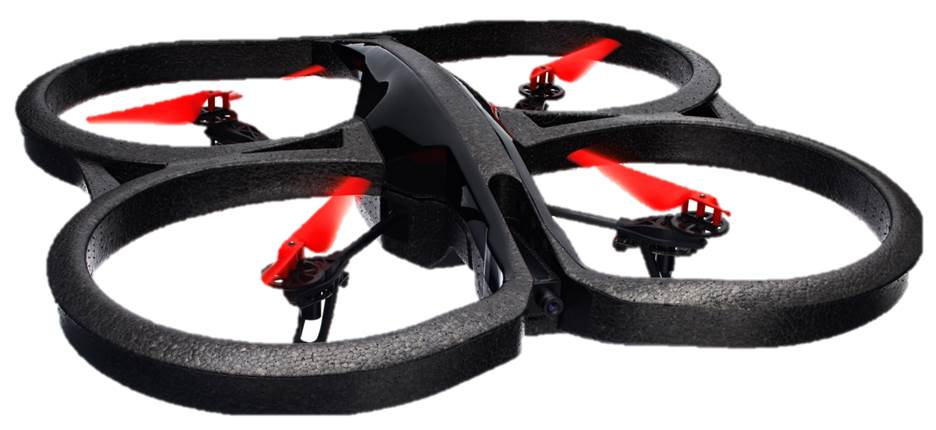
\includegraphics[width=0.3\linewidth]{images/ardrone2}	
  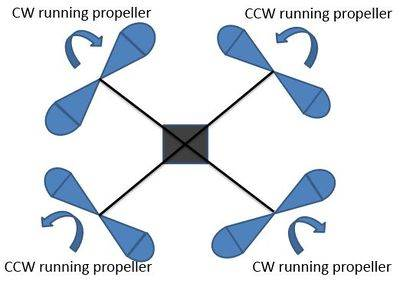
\includegraphics[width=0.34\linewidth]{images/quadrotor}
  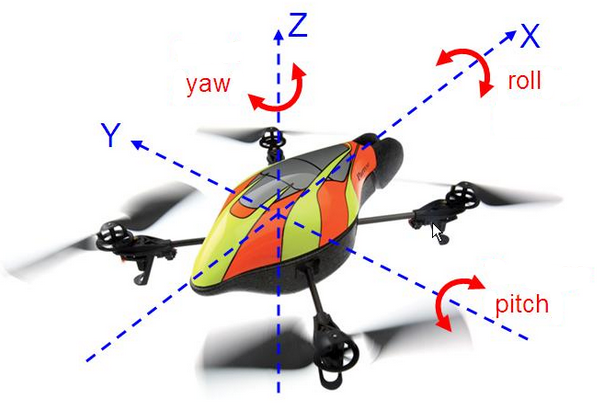
\includegraphics[width=0.34\linewidth]{images/rpy}
  \caption[Quadcopter Motions]{Left: Sample quadcopter, Parrot's ARDrone 2.0.
  Middle: Direction of propeller movement of quadcopter. Right: Rotation of
  quadcopter along three axes. [Picture Courtesy: Google image search]}
  \label{fig:quadcopter}
\end{figure}

The speed of each rotor can be independently varied through onboard flight
controller to achieve various controls. For example, if we would like to hover
the quadcopter, the thrust generated by all rotors should match the weight of the
quadcopter. If we want to move in any direction, then controller tilts the
quadcopter on that side by increasing speed of rotors on other side. The
horizontal component of the thrust will move the quadcopter in that direction.
If we want to rotate the quadcopter around z-axis, i.e., to change its yaw,
controller imbalances the torque purposefully by increasing speed of rotors on
one diagonal. For e.g., if we increase speed of rotors which are rotating in
clockwise direction, quadcopter will turn in counterclockwise direction.
This is illustrated in Figure~\ref{fig:quadcopterMotion}.

\begin{figure}[h!]
  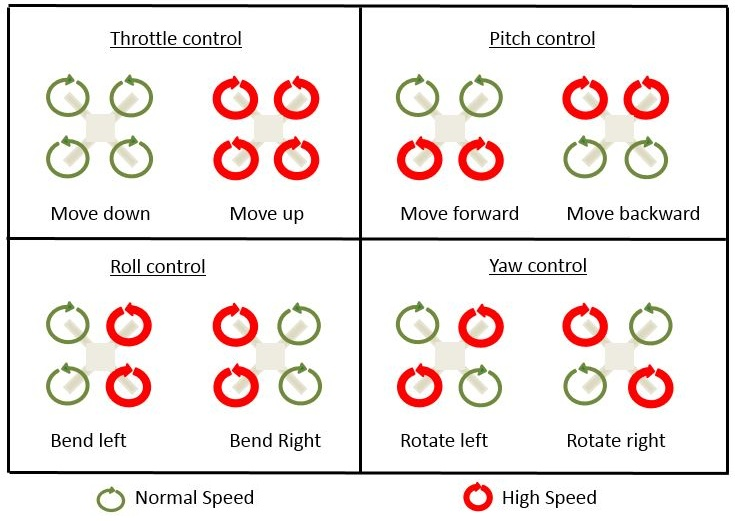
\includegraphics[width=\textwidth]{images/quadcopterMotion.jpg}
  \caption[Speed control of rotors for quadcopter's motion]{Speed control of
  rotors for quadcopter's motion.
  (Left-Top): Speed of all rotors is increased/decreased to move
  quadcopter up/down.
  (Right-Top): To move quadcopter in forward/backward direction, we increase
  speed of rear/front rotors.
  (Left-Bottom): To move quadcopter in left/right direction, we increase
  speed of right/left rotors.
  (Right-bottom): To rotate quadcopter in clockwise direction, we increase speed
  of rotors moving in counterclockwise direction and vice-versa. 
   [Picture Courtesy: Google image search]}
  \label{fig:quadcopterMotion}	
\end{figure}

Quadcopter mainly contains three subsystems: Inertial Measurement Unit (IMU),
Imaging system, and Communication system all connected to Central Processing
Unit, an ARM processor. IMU is responsible for getting the pose of quadcopter.
Imaging system deals with capture and storage of images of surrounding
environment. Communication system handles interfacing between quadcopter and
client device. Here, we have given details of Parrot's AR Drone 2.0 as we are
using the same for our experiments. Though components will remain mostly same across
different quadcopters, technical specifications (e.g., image resolution) may
vary across various models.

\subsection{Inertial Measurement Unit (IMU)}
Every quadcopter has Inertial Measurement Unit (IMU) onboard in order to maneuver
quadcopter in controlled way. IMU is an electronic device which measures forces
acted upon the body of quadcopter. It comprises of 3-axis accelerometer, 3-axis
gyroscope, 3-axis magnetometer, and ultrasound altimeter (also called as sonar).
Accelerometer measures acceleration of quadcopter along 3 axes while gyroscopes
measures angular movement around 3 axes, i.e., roll, pitch and yaw. Magnetometer
measures angular movement with respect to magnetic axis of earth, to get
absolute angle from magnetic axis. Sonar measures quadcopter's
height from the ground.

Sometimes IMU also have pressure sensor to measure the air-pressure around the
device. It is helpful in checking if there is a strong wind so that
onboard flight controller can take the corrective action to stabilize the
quadcopter. 

IMU provides us information about linear as well as angular accelerations. This
information is later used to estimate the pose of the quadcopter. However, due
to various factors such as noisy measurements, environmental disturbances, the
estimated pose may be completely off.
 
\subsection{Imaging System}
Parrot's ARDrone 2.0 has two cameras, front camera with a wideangle lens
($92^{\circ}$ diagonal) to capture images with HD resolution (1280 $\times$ 720
pixels) at 30 FPS, while vertical camera (pointing downwards) having QVGA
resolution (320 $\times$ 240) at 60 FPS used for measuring ground speed.
Though front camera can capture the images at HD resolution, it can transmit
images over Wi-Fi at only  lower resolution (640 $\times$ 360 pixels). Hence we
need to use USB storage device on quadcopter to store a video streamed by the
quadcopter camera. 

\subsection{Communication System}
The AR.Drone 2.0 can be controlled from any client device supporting WiFi. The 
process followed is :
\begin{enumerate}
  \item The AR.Drone creates a WiFi network with an SSID usually named
adrone2\_xxx (where xxx is manufacture date in YYYYMMDD format) and self
allocates a free, odd IP address (typically 192.168.1.1).

   \item The user connects the client device to this SSID network.
   \item The client device requests an IP address from the drone DHCP server.
   \item The AR.Drone DHCP server grants the client with an IP address which is
   the drone's own IP address plus a number between 1 and 4 e.g., 192.168.1.3
   \item The client device can start sending requests (Land, Takeoff, etc.) to
   the AR.Drone IP address and its services ports
\end{enumerate}

ARDrone 2.0 can be controlled from client device through 3 main communication
services: 
\begin{itemize}
\item \textit{AT} commands for control and configuration are sent on UDP
port 5556.
\item Information about the drone (like its status, position,  speed, 
etc.), called as \textit{navdata}, is sent by the drone to its client on UDP
port 5554.  
\item A video stream is sent by the AR.Drone to the client device on UDP port
5555.
\end{itemize}

Now, we will see prior work done in the field of quadcopter navigation,
mosaicing of scenes, and tracking of quadcopter.

\section{Control and Navigation of quadcopter}
In this section we will discuss manual as well as autonomous ways to navigate
a quadcopter, specifically Parrot's ARDrone 2.0.
Parrot has released an mobile app, AR.FreeFlight on iPhone as well as Android
phones for piloting ARDrone. This App can be used to do simple maneuvers such
as going left/right, forward/backward, up/down. It also has a ``Director mode'',
which allows some advanced maneuvers such as circling around itself to take
panoramic view. But still it is very difficult to maneuver the drone without
expertise.

\begin{figure}[h!]
  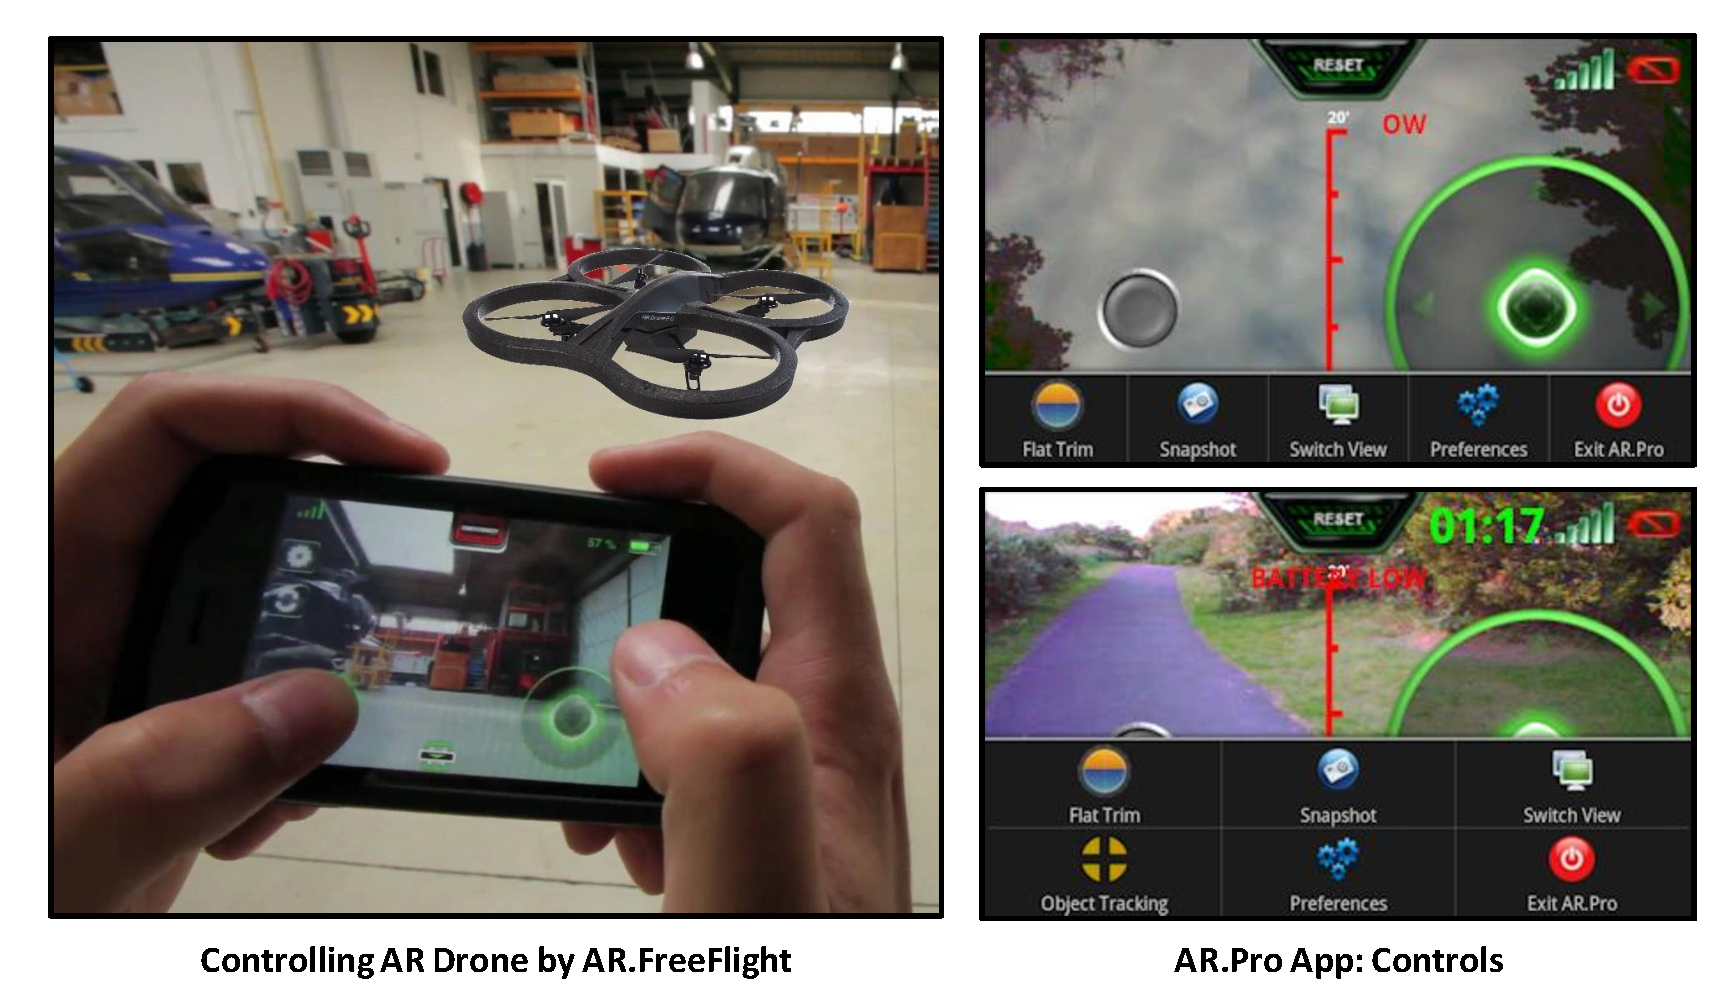
\includegraphics[width=\textwidth]{figures/manualControl}
   \caption[Manual control of Parrot's ARDrone 2.0]{Manual control of Parrot's
  ARDrone 2.0 through smartphone. Left: Parrot's AR.FreeFlight is used to
  control the ARDrone 2.0. 
  Right: Alternatively one may use AR.Pro having advanced features for control.
  [Picture Courtesy: Google image search]}
   \label{fig:manualControl}
\end{figure}

There are also some paid apps such AR.pro for piloting AR Drone. AR.pro app
have some advanced settings which are not available in AR.Freeflight e.g.,
changing WiFi channel, Altitude limiter, Dual Joystick support, etc. All of
these apps as well as softwares have main limitation that as it involves lot of manual
intervention, it lacks precision, which is required in imaging application.
E.g., if we want quadcopter to complete a rectangular loop and come back to its original
position, it fails to do so. 

Some flight controller softwares use add-on GPS for autonomous navigation of
quadcopter. However in GPS denied areas e.g., indoor, we can not use such
softwares. Even in outdoor, we cannot rely on only GPS for accurate
navigation of quadcopter due to issues like spurious GPS signals, GPS jammers,
etc.

Another way to accurately navigate quadcopter is to use techniques such as
Simultaneous Localization And Mapping(SLAM)\cite{Davison:2007} or Parallel Tracking And
Mapping(PTAM)\cite{klein}. SLAM or PTAM algorithm first builds a 3D map of
surrounding environment and then estimates device's current position.

Engel et al.~\cite{Engel12} have developed a method for navigation of quadcopter
based on PTAM\cite{klein}. Engel et al. have used Extended Kalman Filter (EKF)
to fuse visual observation model with the odometry observation model to estimate
the pose of the quadcopter. They have also developed a method for
correctly estimating scale of the built 3D map. But, they have not ensured
a hundred percent scale accuracy which results in an inaccurate 3D map of
the surrounding environment.

\section{Mosaicing of scenes}
Panoramic image stitching (alternatively, image mosaicing) is a
well-studied problem in the field of computer vision.  Representative
works include~\cite{Milgram1975}, \cite{Milgram1977}, \cite{Capel},
\cite{Szeliski1997}, \cite{Brown07}, \cite{Brown03}.  A full discussion
on related works is outside the scope of this work, readers are
referred to~\cite{Szeliski05imagealignment} for an excellent survey.
Given the maturity of this area, there are various freeware as well as
commercial software available for performing image stitching; most
notable are AutoStitch \cite{autostitch}, Microsoft\textsc{\char"13}s Image
Compositing Editor \cite{ICE}, and Adobe\textsc{\char"13}s Photoshop
\cite{photoshop}.

All of these methods are based on a similar strategy of finding
features in each image, matching these features between images, and
then computing pairwise image warps to align them together.  A 
bundle adjustment is often applied to globally refine the alignment.
All of the aforementioned methods assume the imaged scene is planar or
that the camera has been rotated carefully around its center of
projection to avoid parallax.

Brown \etal \cite{Brown05} have used a new type of invariant features
located at Harris corners in discrete scale-space and oriented using a
blurred local gradient for stitching. Eden \etal \cite{Eden} were
able to stitch images with large exposure difference as well as large
scene motion into single HDR quality image without using any
additional camera hardware.

All of the image mosaicing methods work only when there is an
``intersection'' in feature space of images to be stitched. When there
are ``gaps'' (either physical or due to lack of features) between
images to be stitched it is not clear how to perform the
stitching. Structure from Motion methods also rely on overlap of
features and fail when images have gaps. In this work, we discuss how
to use the available IMU data that accompanies our input images to
help overcome these problems.

\subsection{Mosaicing of Aerial Imagery}
There is a lot of work happened in the area of mosaicing aerial images
captured from UAVs as well as mosaicing of remotely sensed images from satellites.
Representatives of these works are \cite{Yue, Yuanhang, Yahyanejad, Zhu}.
These works use UAVs to image ground scenes from heights (minimum 100 ft.
above from ground). However we are interested in imaging scenes from much closer
distance for application such as inspection of walls or towers. Intricacies
involved in imaging such surfaces from closer distance are different than aerial
imaging. Hence, we \textit{cannot} use methods used for mosaicing of aerial 
imagery in our problem.
\section{Fiducial Markers and Tracking}
Inexpensive quadcopter such as Parrot's AR Drone have very jerky movement. Hence,
it is difficult to track the objects through quadcopter or even the quadcopter
itself. In this section we will review the prior work done related to the
tracking aspect of the quadcopter.\\

\noindent\textbf{Fiducials:}~Fiducials are often used to evaluate the planning
algorithms given that ground truth positions can be detected by the
quadcopter's camera. Figure~\ref{fig:previous_work} shows a few
examples of existing fiducials.  Many designs use a two
dimensional barcode inside a rectangular grid. One example of such a
fiducial is from the ARToolkit~\cite{ARToolkit02}, a well known
toolkit used in many augmented reality (AR) applications. Kato and
Billinghurst~\cite{kato-artoolkit} first demonstrated the use of
ARToolkit in various augmented-reality-based applications.

\begin{figure}[b!]
\centering
 \begin{subfigure}[b]{0.29\linewidth}
  \centering
  
\includegraphics[width=0.8\linewidth]{figures/fiducial/intersense.jpg}
  Circular Data Matrix~\cite{NaimarkF02}
 \end{subfigure}\quad
 \begin{subfigure}[b]{0.2\linewidth}
 \centering
  
\includegraphics[width=\linewidth]{figures/fiducial/pattKanji.pdf}
  ARToolkit~\cite{ARToolkit02}
 \end{subfigure}\quad
 \begin{subfigure}[b]{0.2\linewidth}
  \centering
  
\includegraphics[width=\linewidth]{figures/fiducial/ARtag.jpg}
  ARTag\quad~\cite{Fiala05}
 \end{subfigure}\quad
 \begin{subfigure}[b]{0.2\linewidth}
  \centering
  
\includegraphics[width=\linewidth]{figures/fiducial/pifiducial.jpg}
  PiTag\quad~\cite{Pitag13}
 \end{subfigure}
 %\quad
%  \begin{subfigure}[b]{0.14\linewidth}
%   \centering
%   
\includegraphics[width=\linewidth]{figures/fiducial/our_fiducial.jpg}
%   Our Fiducial
%  \end{subfigure}
 \caption[Prior fiducials]{Prior fiducials and our proposal. 
 While each code has its pros and cons depending on the environment, no
 prior code is expressly designed to be recognized under motion blur.}
 \label{fig:previous_work}
\end{figure}


Fiala~\cite{Fiala05} proposed a fiducial termed, ARTag, which is a
bi-tonal system consisting of a square border and an interior
6$\times$6 grid of black or white cells. The improvement of the ARTag
compared to the ARToolkit lies in the detection of corners instead of
detection of lines to find possible patterns.  This proved to be more
efficient than \cite{ARToolkit02} in terms of recognition rate as well
as the number of different patterns which can be created.  {\it The
reliance on both line and corner detection, however, hampers
recognition under motion blur.}

There were also attempts to use circular patterns instead of
rectangular.  Gatrell et al.~\cite{concentric} used concentric circles
for monocular pose estimation as well as object identification. Cho et
al.~\cite{Cho:2001,Cho97fastcolor} have used multicolor rings instead
of black and white rings~\cite{concentric} to increase possible number
of fiducials.  These multicolor rings are used in wide area tracking
in large scale applications.  {\it Although based on  concentric rings, these
approaches require the complete ring to be recognized; this is
impractical when the pattern undergoes directional motion blur.}

Naimark and Foxlin~\cite{NaimarkF02} proposed a circular bar code
called the Circular Data Matrix that is beneficial in terms of easy
detection and ability to have a large number of uniquely identifiable
codes.  To address the issue of occlusion, Bergamasco et
al.~\cite{runetag11} proposed the RUNE-tag fiducial by creating a
number of circular dots arranged in circular fashion. RUNE-tags can be
detected even when 50\% of the fiducial area is occluded. Bergamasco
et al.~\cite{Pitag13} proposed the PiTag fiducial, also composed of
circular structures but arranged in a rectangle, to exploit projective
invariant cross-ratio.  This provided similar occlusion resistance as
RUNE-tag but with even less circular dots. {\it All of these techniques,
however, rely on generic feature detection (e.g., circle detection)
and such algorithms break down under motion blur.}\\

%Zhang et al.\cite{Zhang:2002} and Claus et al. \cite{ClausF04} have done
%quite comprehensive comparative study of various fiducial systems with
%respect to processing time, recognition rate and accuracy with
%respect to viewing angle and distance.

\noindent{\textbf{Tracking:}}~~Fiducial detection between successive video
frames can be considered as a tracking problem where the tracked
object is the fiducial.  There is a very large body of research
dedicated to tracking and interested readers are referred
to~\cite{Yilmaz:2006} for a good survey.

Most tracking methods~\cite{Ross:2008,Wu:2009,Perez02,Mei:2009} assume
the image sequence to be blur free. In reality, however, the presence
of motion blur in a video sequence is often unavoidable. To this end,
Wu et al.~\cite{Wu:2011} proposed the Blur-driven Tracker (BLUT)
framework for tracking motion-blurred targets. BLUT is based on the
observation that although motion blur degrades the visual features of
the target, it may also provide useful cues about the movements to
help tracking.

The BLUT framework successfully tracks a blurred target when there is
uniform motion, and the position of the tracked object does not change
drastically in successive frames. However, the erratic motion from the
quadcopters, as well as the problem of dropped video frames makes the task too
problematic for BLUT to successfully track.

In this chapter, we got acquainted with quadcopter, motion control, its
components. We also have seen limitations of existing methods for quadcopter
travel and imaging.  We will discuss how these limitations are addressed in
upcoming chapters.
\chapter{Mosaicing Scenes with  Vacant Spaces}
\label{ch:vacantSpaces}
Finding features and using them to align images to construct wide
field of view panoramas is one of the success stories of computer
vision.  Virtually all recent consumer cameras have this technology
embedded.  The success of these methods relies significantly on
finding common features in the images that can be used to establish
the appropriate warps to register the images together.

\begin{figure}
  \centering
  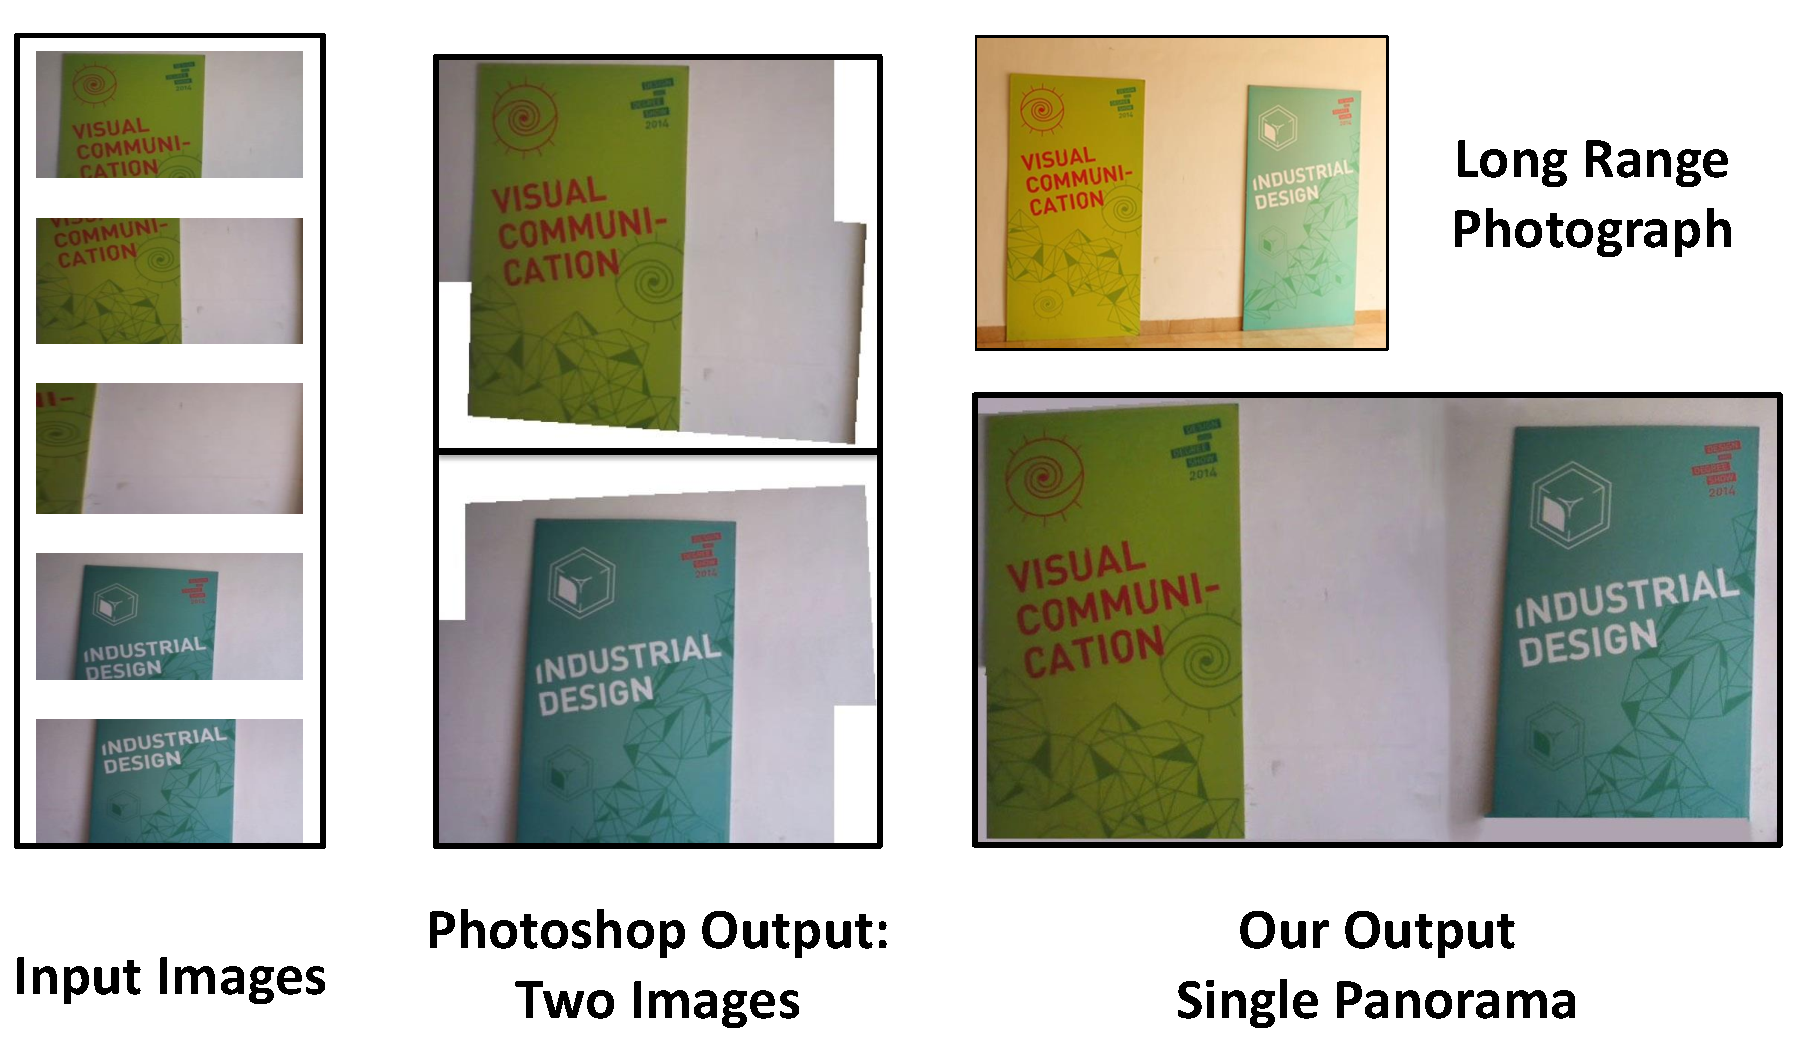
\includegraphics[width=0.8\textwidth]{figures/vacantSpaces/teaser.pdf}
  \caption[Overview]{ \label{fig:teaser} The long range photograph of a scene
    taken from an SLR camera is shown in top right.  When such a scene
    is probed by a quadcopter, it results in the input images shown on
    the left (color balance is different from the SLR camera).  The
    state of the art methods (middle column) are unable to make a
    \emph{single} mosaic because the vacant space (third picture on
    the left) does not seem to have any matchable features with
    subsequent input images. Our method handles this situation (bottom
    right).  }
\end{figure}

There are scenes, however, that consist of image content that makes
this challenging.  One situation is when the scene needs to be probed
in an orthographic view, and is not easily accessible.  Murals on
urban architecture is an example. Another situation is when scene
patterns and texture are repeated (too many similar features in, e.g.,
an outdoor art exhibition).  This can make it challenging for a
matching algorithm to find appropriate matches in large panoramas.  A
related situation is when a scene area simply does not contain
features (too little, or no features, e.g. posters in an event).
Fig~\ref{fig:teaser} shows an example of this case.  The state of the
art methods are unsatisfactory.  The idea of a moving quadcopter
taking pictures suggests using a Structure from Motion (SfM) paradigm.
However, based on our experiments with Bundler\cite{Snavely06,
  Snavely07} and VisualSFM \cite{Wu13}, we see that the success of SfM
depends very strongly on ``good'' correspondences between input
images, absent in large vacant (featureless) spaces (please see supplementary 
material).  Specialized -- state of the art -- image stitching 
methods from \cite{Brown03, Brown05} used in tuned software like Adobe 
Photoshop CS6 or AutoStitch \emph{also} do not work as can be seen 
in Figure~\ref{fig:teaser}.


The goal in this work is to create panoramic images of scenes using a
quadcopter in situations described above. From a vision perspective,
we are excited about a new mosaicing problem containing large
homogeneous vacant spaces.  This results in scene regions that have no
matches between many significant images, and therefore cannot be
aligned using traditional mosaicing methods.


{\bf Key Idea} We propose to solve the vacant space problem by using
an inexpensive off-the-shelf flying device, such as a quadcopter which
can be assumed to contain an inertial measurement unit (IMU) that has
positional information.  The proximity relationship that the resultant
images have, can be used to significantly reduce the search space in
finding matches.  Further, the proximity relationship also allows, in
principle, to vary the parameters involved in feature selection. For
example, if there is reason to believe that two images are adjacent
horizontally, one can choose to adjust thresholds in feature matching
algorithm to hunt for otherwise elusive matching pairs.

We note that IMU data can be also made available in other devices such
as smartphones.  An autonomous programmed quadcopter, however, is
particularly enticing because of its ability to fly to areas that are
accessible to the human eye, but inaccessible for the human to
reach. Such areas do not lend themselves easily to high quality
images. 

Further, IMU data, whether on a smartphone or on a quadcopter, cannot
be relied exclusively, or sometimes at all, especially on inexpensive
devices. Our experiments indicate that the roll and pitch angles
(depending on the distances involved) may be completely off, and so
can the physical coordinates.  This is a consequence of the jerky,
swift movements.  Complementing the IMU with information gleaned from
vision algorithms, however, may be a useful practice.

{\bf Contributions} The main technical contribution of this work is
that it improves the state of the art in mosaicing.  We assume that
the imagery is acquired by a quadcopter for the reasons mentioned
above. Sending a battery of images from a quadcopter to an image
mosaicing algorithm such as AutoStitch incapacitates the algorithm
because of the sheer number of images. Sending a sampled version of
images to a manageable number $N$ of images, with $O(N^2)$ possible
areas to match for features, also does not work since the sampled
image contains vacant space.  In this work, we use IMU information
that lends itself to a graceful $O(N)$ algorithm.  Results are
available in the experiments section. In summary we have a solution to a new problem, and a
faster solution using IMU data.

%{\bf Limitations} 
In this work, we assume that the scene lies on a planar surface, or
approximately planar surface. The quadcopter can also be programmed to
have a viewing angle perpendicular to any desired planar structure.
The standard homography computation is still not possible because of
the vacant spaces. To overcome this, we reduce the mosaicing problem
to the stereo problem and are thus able to complete the panorama.

% The rest of this paper is organized as follows.  In the next section,
% we discuss related work.  Subsequently we describe the main steps in
% our process, and justify the process in Section~\ref{sec:results} with
% experimental results. (Additional results are available in
% supplementary material.)  The final section discusses future work.

\section{Methodology}

The goal of this work is to compute a panorama of a scene lying on
planar surface that has regions of vacant spaces.  A schematic for
this problem is shown in Figure~\ref{fig:schematic}. 

\begin{figure}[h!]
  \centering
  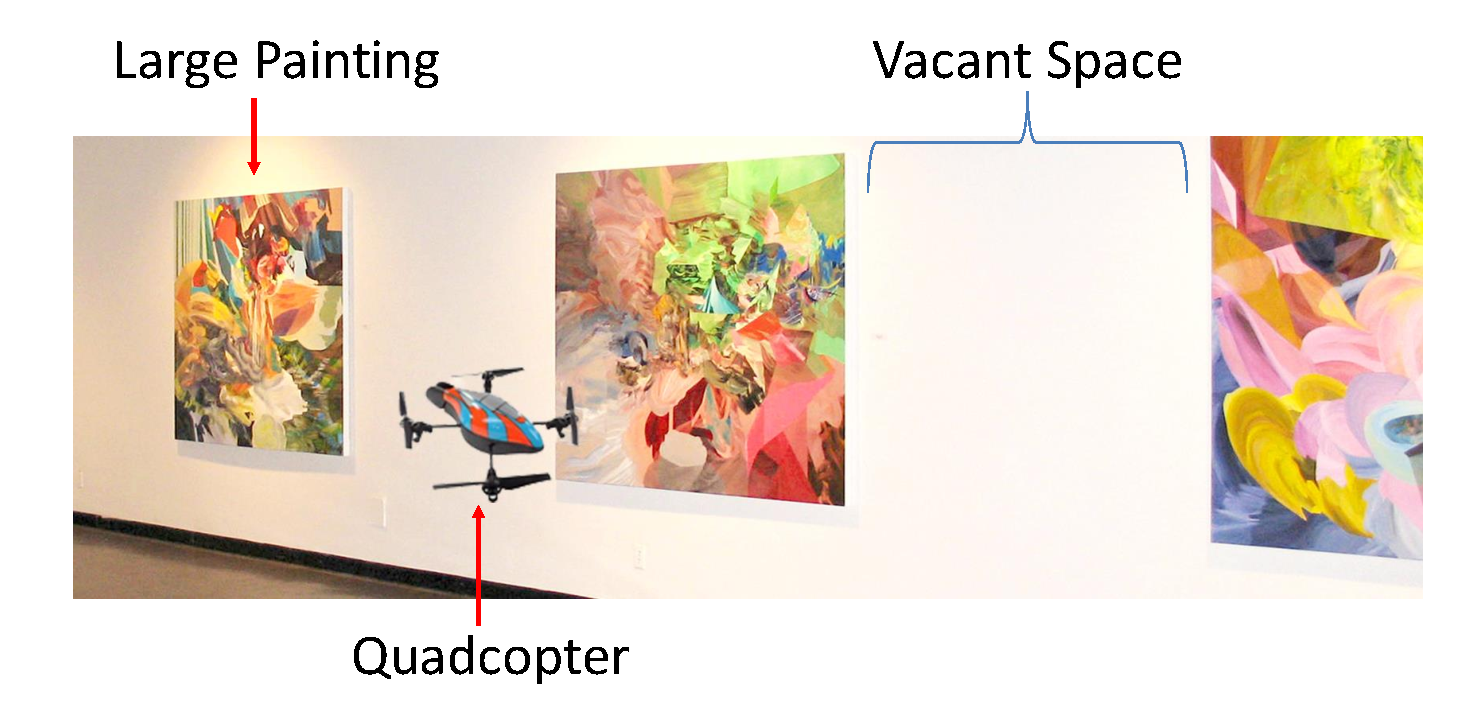
\includegraphics[width=0.8\textwidth]{figures/vacantSpaces/indoor}\\
  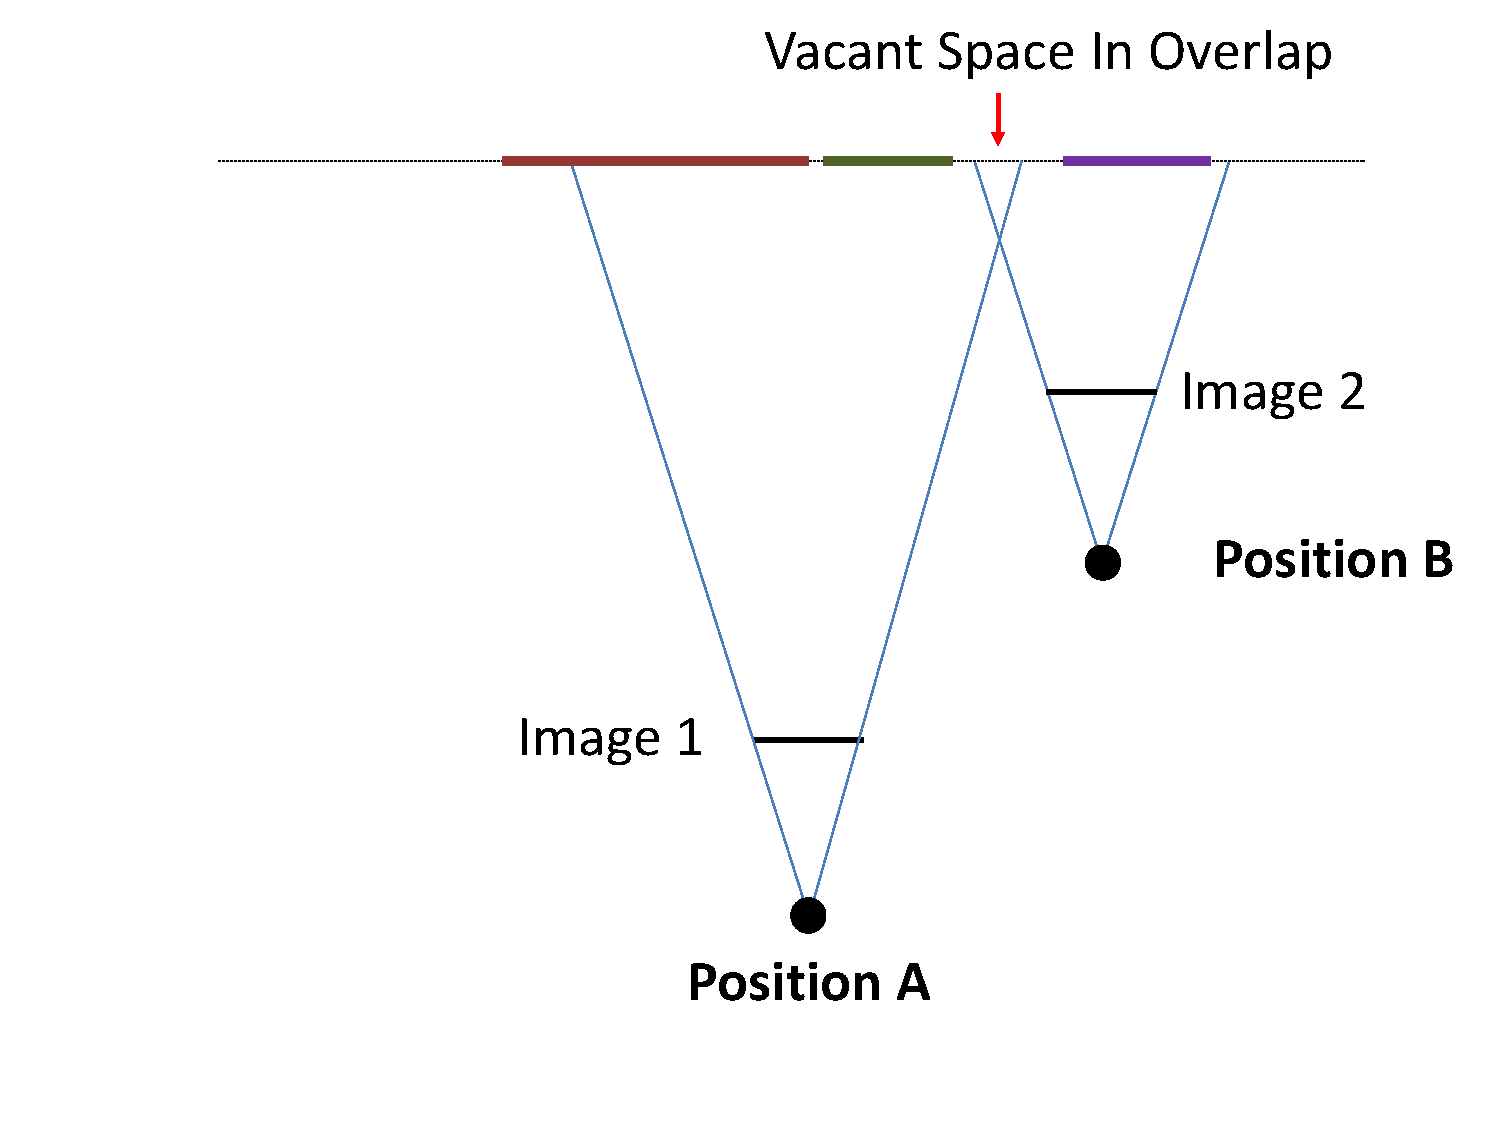
\includegraphics[width=0.8\textwidth]{figures/vacantSpaces/stereoOverlap}\\

  \caption[Problem definition]{ \label{fig:schematic} Problem definition. (Top)
  Vacant spaces are encountered in various scenes.  When individual portions are
    captured by a quadcopter, how does one create the complete mosaic
    given that common features are either not available, or
    confusing? (Bottom) Simplified reduction of the problem to a geometrical structure.
  }
\end{figure}    

The method adopted is pictorially depicted in the overview shown in
Figure~\ref{fig:workflow} and is described in detail later on.  In
brief, we systematically acquire a video of the scene, reduce the
input video to a manageable number of images, and finally combine the
images acquired from different positions into a mosaic.

\begin{figure}[h!]
  \centering
  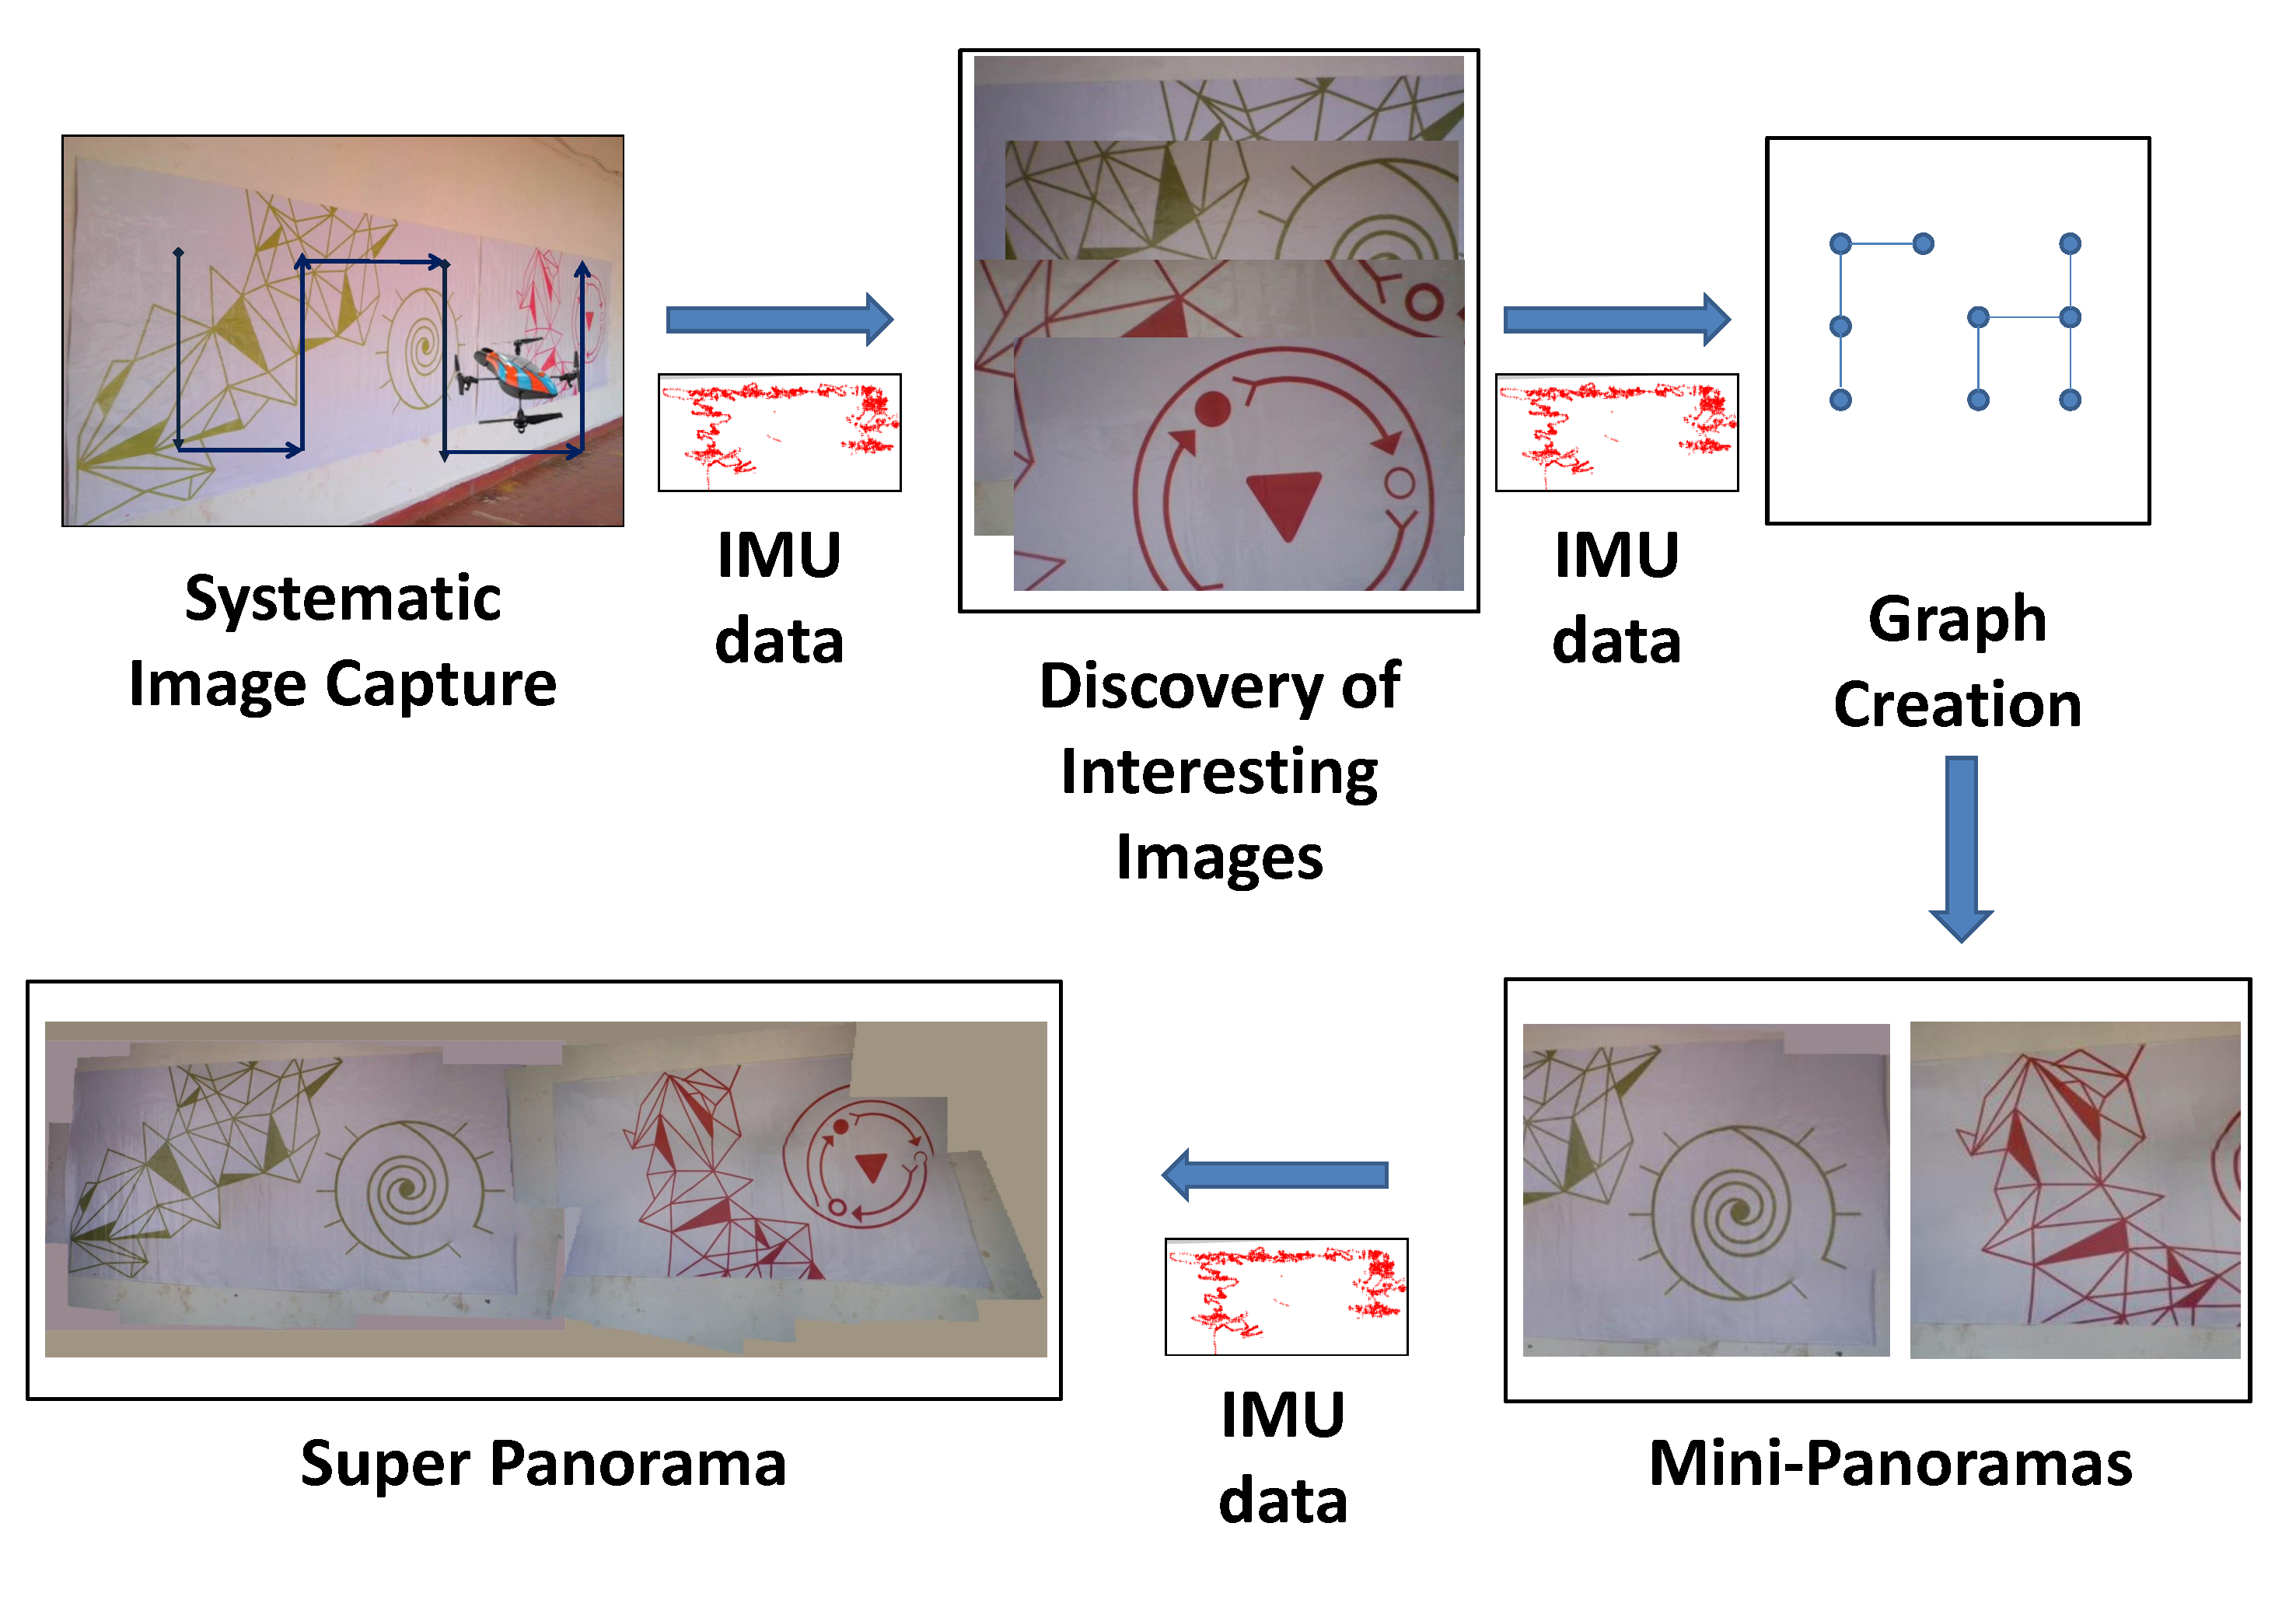
\includegraphics[width=\textwidth]{figures/vacantSpaces/Workflow} 
  \caption[Workflow]{ \label{fig:workflow} Overview: Input imagery is
    systematically acquired (top left) by a quadcopter.  In the next
    step, interesting images are found by clustering the video into
    regions based on positional data.  A graph is constructed using
    proximal images. For each connected component in a graph, standard
    stitching techniques are used to create mini-panoramas which are
    then joined together into super panorama 
    again using IMU data.}
\end{figure}    


\subsection{Video acquisition}
We first despatch the quadcopter to as close to the scene as
possible. The corners of a rectangular area of interest are provided
to the quadcopter, and it is programmed to traverse the area in a
raster scan fashion.  There are various control aspects involved in
sending a quadcopter; in outdoor areas, the quadcopter is impacted by
wind and it might lose its way.  The control aspects of the quadcopter
is beyond the scope of this work.  \emph{Note that trying to create a
  mosaic in an incremental linear fashion by combining adjacent frames is
  prone to loss of two-dimensional spatial proximal information. It is also
  computationally overwhelming.}

The quadcopter returns with a video of the scene.  Images extracted
from a short video of about a minute or more overwhelms existing
mosaicing software, such as AutoStitch or Adobe Photoshop.  In the
rest of this section, we use AutoStitch to indicate state of the art
stitching programs such as AutoStitch, Photoshop, etc.

\subsection{Acquiring interesting images}
\label{sec:selection}
Our goal in this step is to reduce the amount of input data and
produce a set of interesting images.  In other words, we wish to
convert a video into an album of images.  The key difference between
our problem and standard albumization \cite{Aner, Lee} is the use of
positional information.  A standard quadcopter has an inertial
measurement unit (IMU) that, after calibration, may give reasonably
accurate information of positions. Using positional information it is
possible to cluster the images, and sort the images into an $m\times
n$ grid.  The number of cluster centers is automatically determined
using the agglomerative bottom up hierarchical clustering method
\cite{Lior}, with the additional requirement that the whole scene
(represented by the positional data) is covered.

{\bf Clustering Details} We assume that each IMU data position
corresponds to an image of definite fixed dimensions.  Consider each
position of the IMU data to be a leaf node. Two nodes are greedily
combined based on the closest Euclidean distance, and replaced with an
internal node; the position of the internal node is set to be the
centroid of the two nodes, and each internal node now corresponds to a
virtual image of the same size taken by a virtual quadcopter.  The
algorithm recursively merges all the nodes till we end up with a root.
In the next phase, we produce cluster centers; a set of nodes is
considered for being the output as cluster centers if the union of
these nodes completely cover the scene. From the bottom-up
construction, it is clear that the root will represent a single
position, and thus a single virtual image, and will not cover the
scene.  At the other extreme, the set of all leaf nodes \emph{will}
cover the scene. To resolve this, during the calibration phase, we
pre-decide the minimum distance between two center of projection to
have least overlap. This is used as the threshold in the clustering
algorithm.  Once cluster centers are found, we pick the leaf node
which is closest to the cluster center to find a real image. This
process is schematically shown in Figure~\ref{fig:selection}.

Remarks: If we had no IMU information, one may consider selecting a
set of interesting images using any appearance based method such as
optical flow or feature selection.  However, due to the jerky and
uneven motion of the quadcopter, such measures do not prove to be
sufficient. On the other hand, on inexpensive quadcopters, we have
encountered several cases of erroneous positional information (we note
here that image computations are not on-board the quadcopter and IMU
information is transmitted via WiFi to a host computer).  

% We believe
% that combination of standard vision-based clustering method with the
% clustering based on positional information can be used to either drop
% frames, or to correctly include frames based on image content.

\begin{figure}[t!]
  \centering
  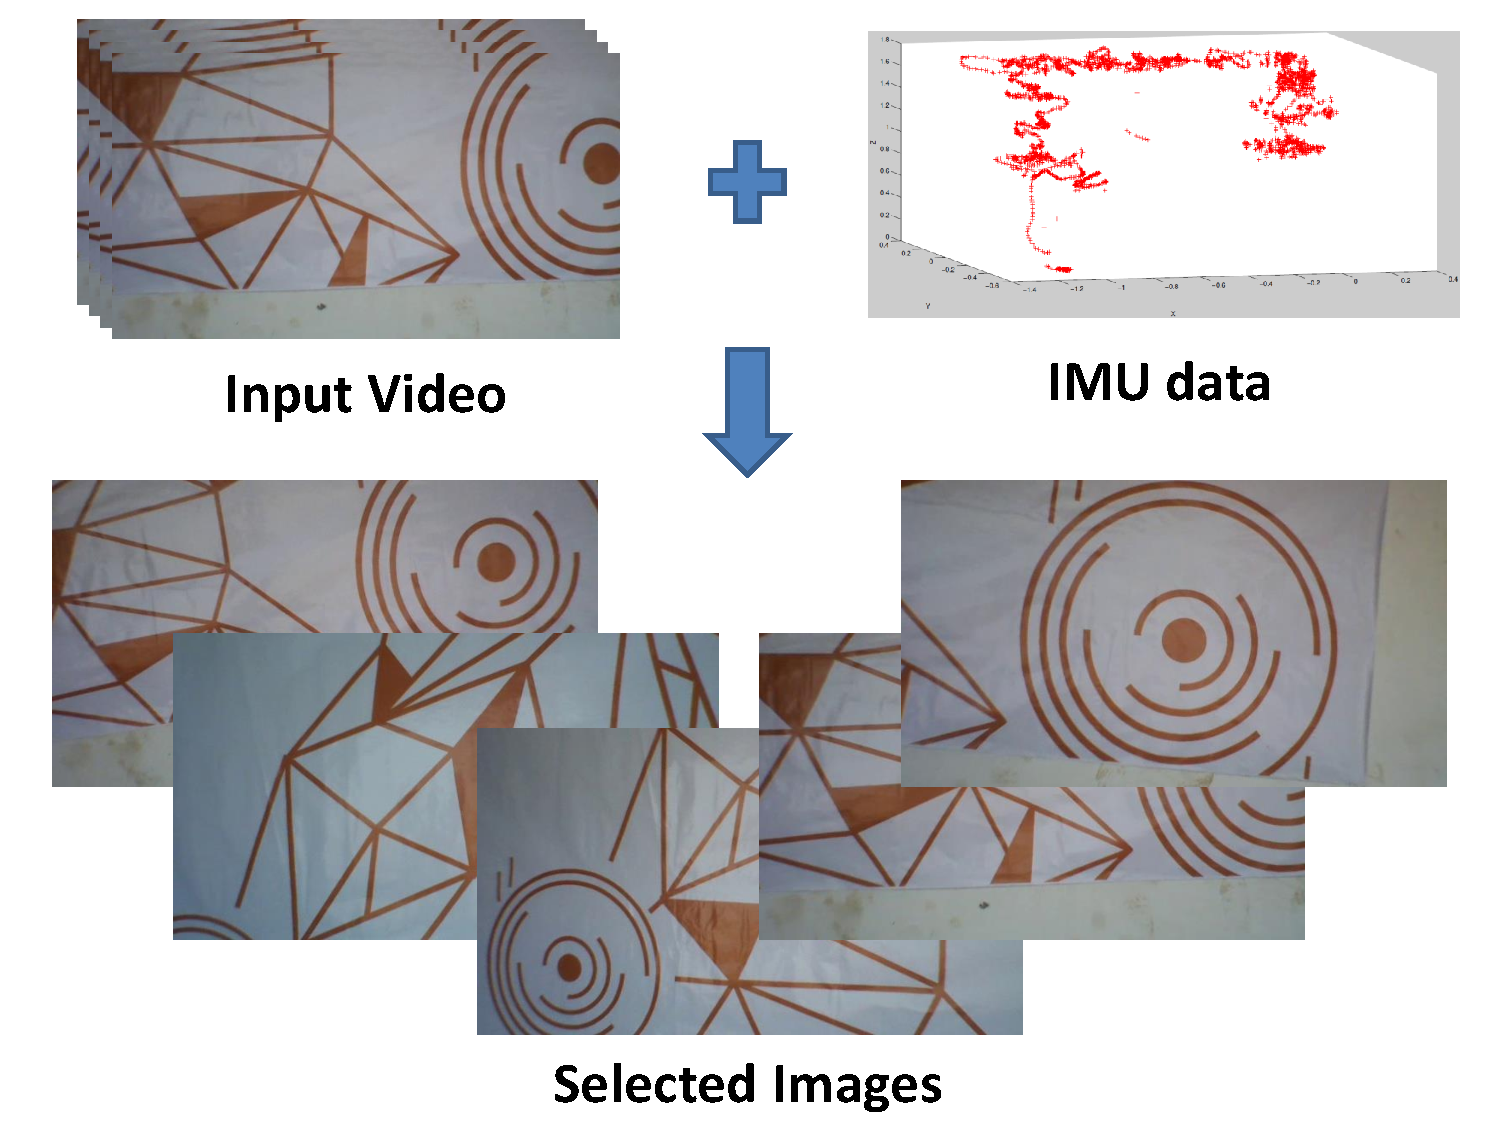
\includegraphics[width=0.8\textwidth]{figures/vacantSpaces/selection} 
  \caption[Selection of Images]{ \label{fig:selection} We align the image stream
  with IMU data, and then transform the video into a set of interesting
    images with a clustering algorithm.}
\end{figure}    

In practice, the number of cluster centers for the scenes we have
covered is now within the capacity of AutoStitch.  As mentioned in the
introduction, as long as there are sufficiently varying and
``matchable'' features, AutoStitch is able to perform a reasonable
result.  However, if there are very few features in overlapping region
of two images, then the output is not acceptable. This situation will
arise when there is vacant space between two pictures.

{\bf Time complexity} AutoStitch has not been designed
to use positional information. As a result if there are $N$ input
images, the program has to consider possible matches in approximately
$O(N^2)$ set of areas.  Our program is able to mosaic in an $O(N)$
fashion.

{\bf Mini-Panoramas} Specifically, we assume at this point that the
interesting photos are available in the form of a $m \times n$
grid. First, we find SURF \cite{Bay} features for each image in a
grid. Next, we use Best of Nearest Neighbor matcher (from the OpenCV
library) with Random Sample Consensus (RANSAC) \cite{Fischler1981} to
find geometrically consistent matches between neighborhood images
inside grid.  We create a graph with images being nodes, and add an
edge between two nodes if there are sufficient matches. We have to
recall at this point that if there are ``vacant spaces'' there will
not be enough features for successful matches; the graph will end up
with multiple (disconnected) components.  We next compute multiple
spanning trees for the various components. Given a spanning tree, the
center of the spanning tree is a node from which the distance to all
other nodes is minimal \cite{Kocay}. Next we calculate the homography
of each image with respect to spanning tree center.  Finally, for each
spanning tree, we stitch all pictures within the spanning tree to
create a mini-panorama using the computed homographies by warping all
images with reference to the image at spanning tree center. The
spanning tree is an $O(N)$ structure. The process is described in
Figure~\ref{fig:graph}.

\begin{figure}[t!]
  \centering
  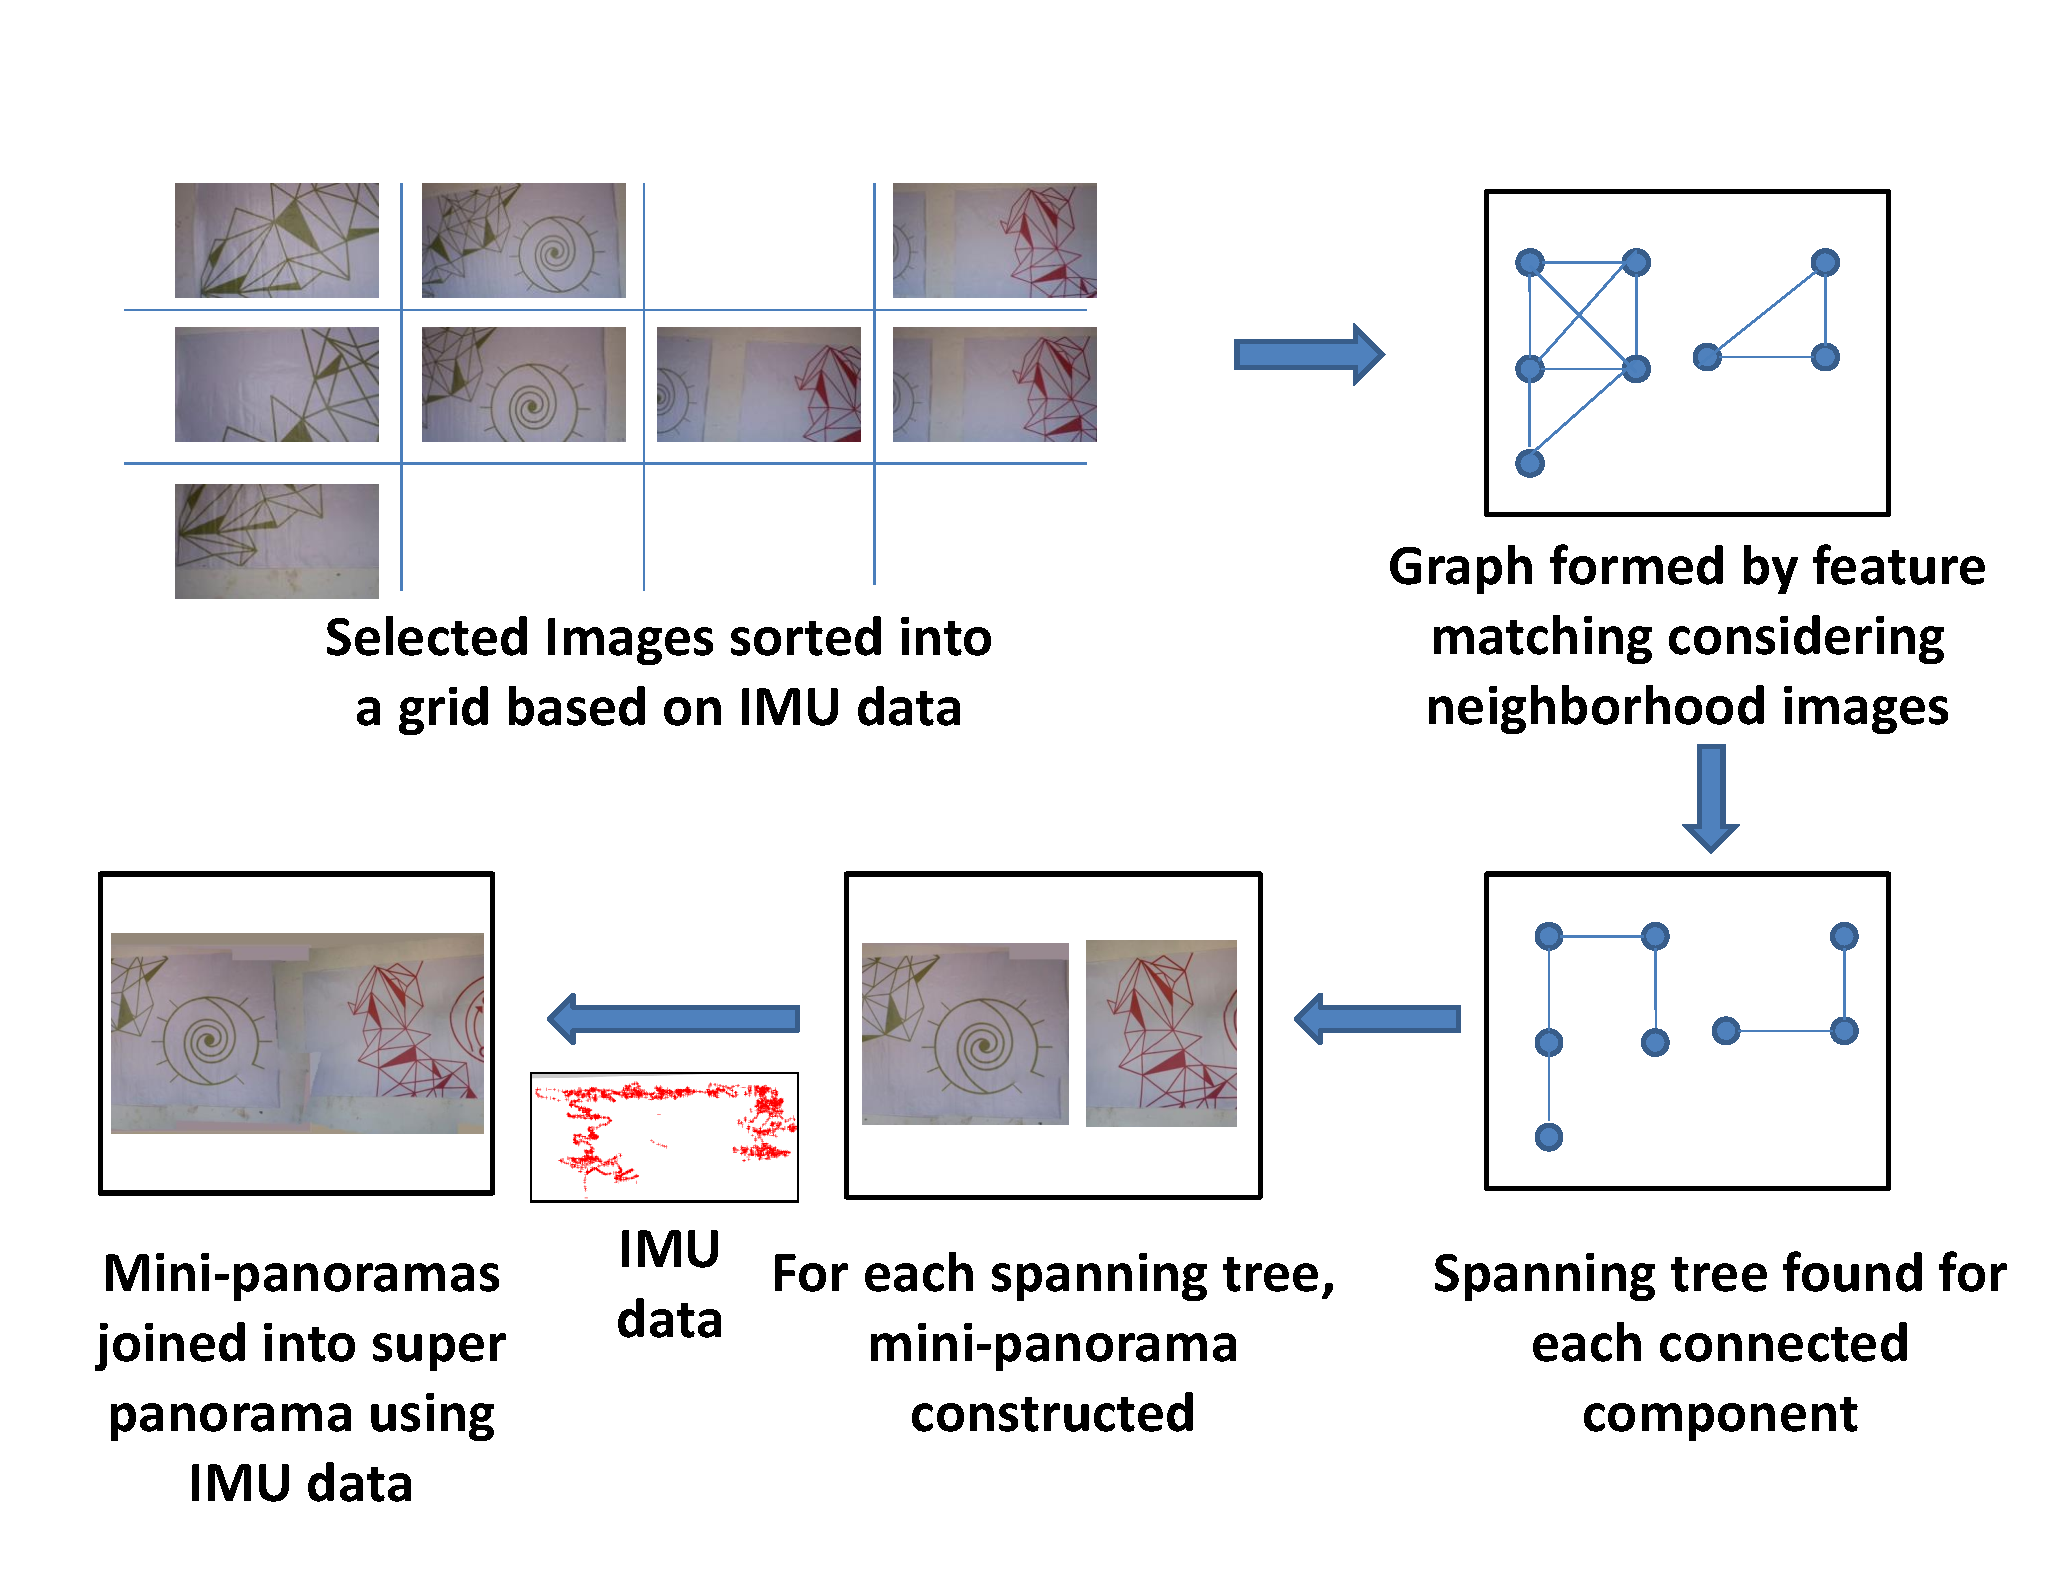
\includegraphics[width=\textwidth]{figures/vacantSpaces/graphCreation} 
  \caption[Creation of Mini-panoramas]{ \label{fig:graph} Interesting images
  acquired are segmented and individual (mini-panoramas) are constructed. These
    are then later combined into the desired super-panoramas using IMU data.}
\end{figure}    

\subsection{Super-panorama}
In this section, we consider the situation when programs like
AutoStitch fail.  We assume that the output of the previous step has
resulted in multiple spanning trees where each spanning tree center
corresponds to a specific depth . This is the depth of the center of
the spanning tree (estimated from the IMU data), since we have stitched all images by taking the
spanning tree center as a reference.  Individual panoramas for each
spanning tree termed mini-panoramas have been created. A
super-panorama must be created from mini-panoramas; these usually
correspond to different depths for at least two reasons.

First, it is invariably difficult, if not impossible, to control a
quadcopter to be at the exact depth even in indoor scenes.  The
aerodynamics and the thrust produced tends to make the quadcopter
drift.  Second, it might also be necessary to let the quadcopter probe
and come closer to the scene so as to get a ``good picture''.

A super-panorama is done using a two step process. Assume two trees in
the forest corresponding to area A and area B of the scene (see
Figure~\ref{fig:stereo}). 
\begin{figure}[h!]
  \centering
  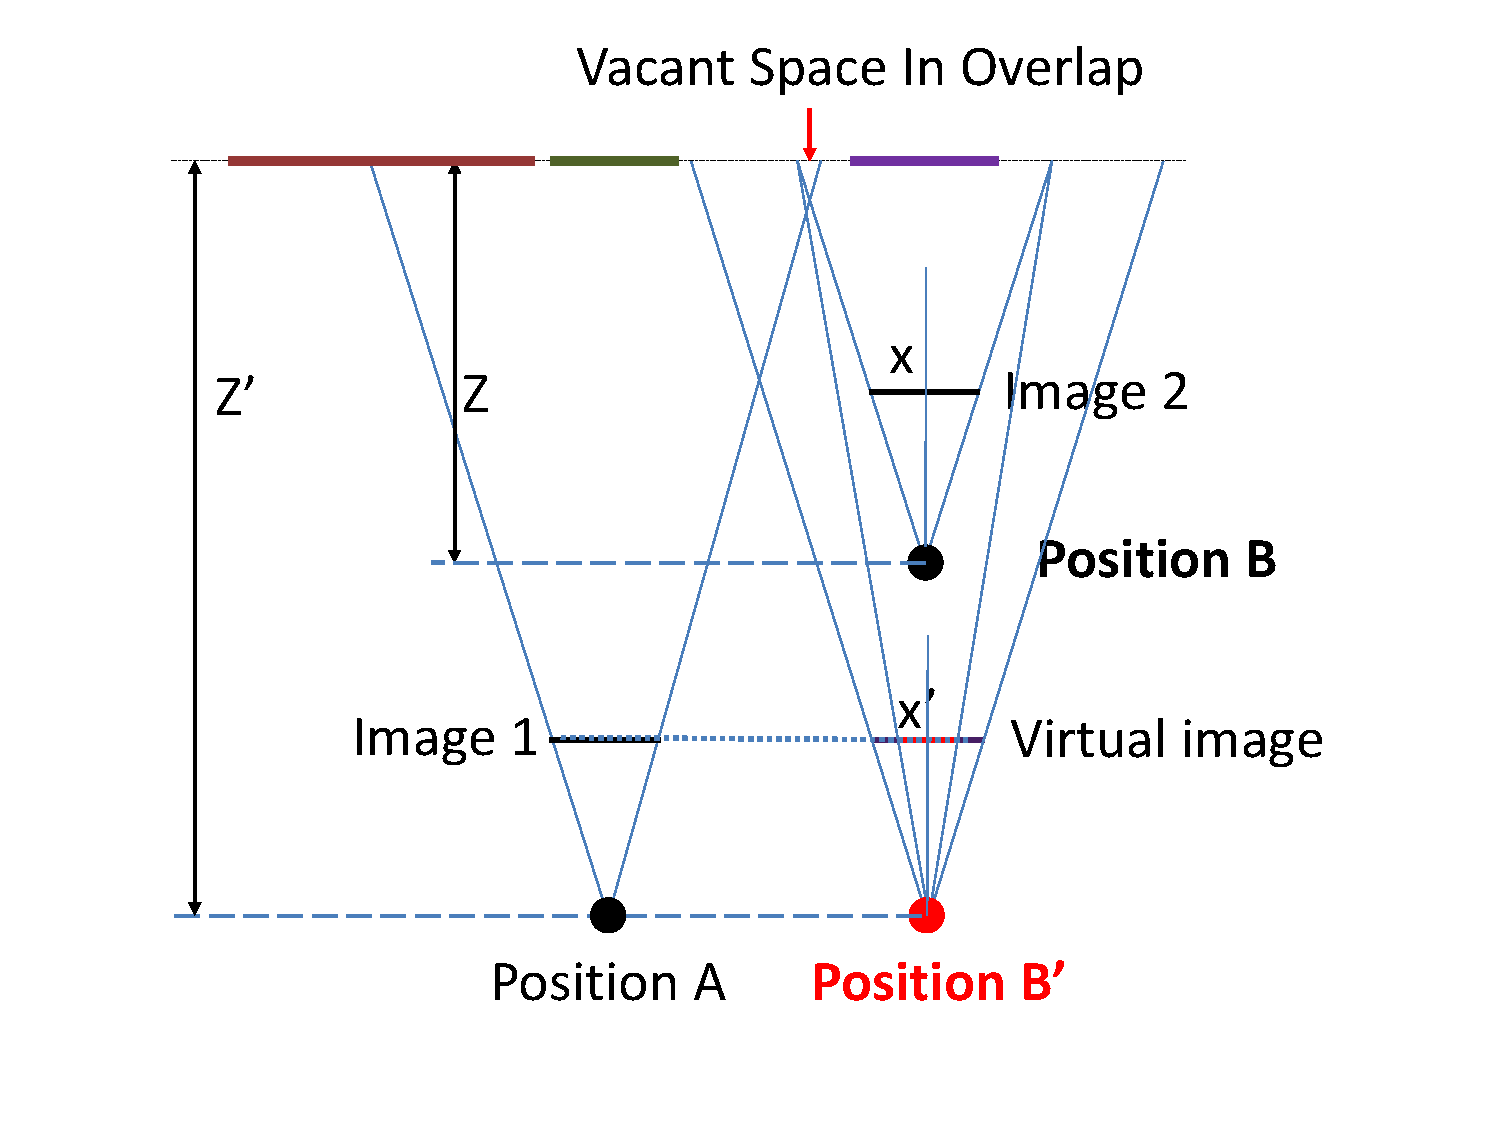
\includegraphics[width=0.8\textwidth]{figures/vacantSpaces/move} \\
  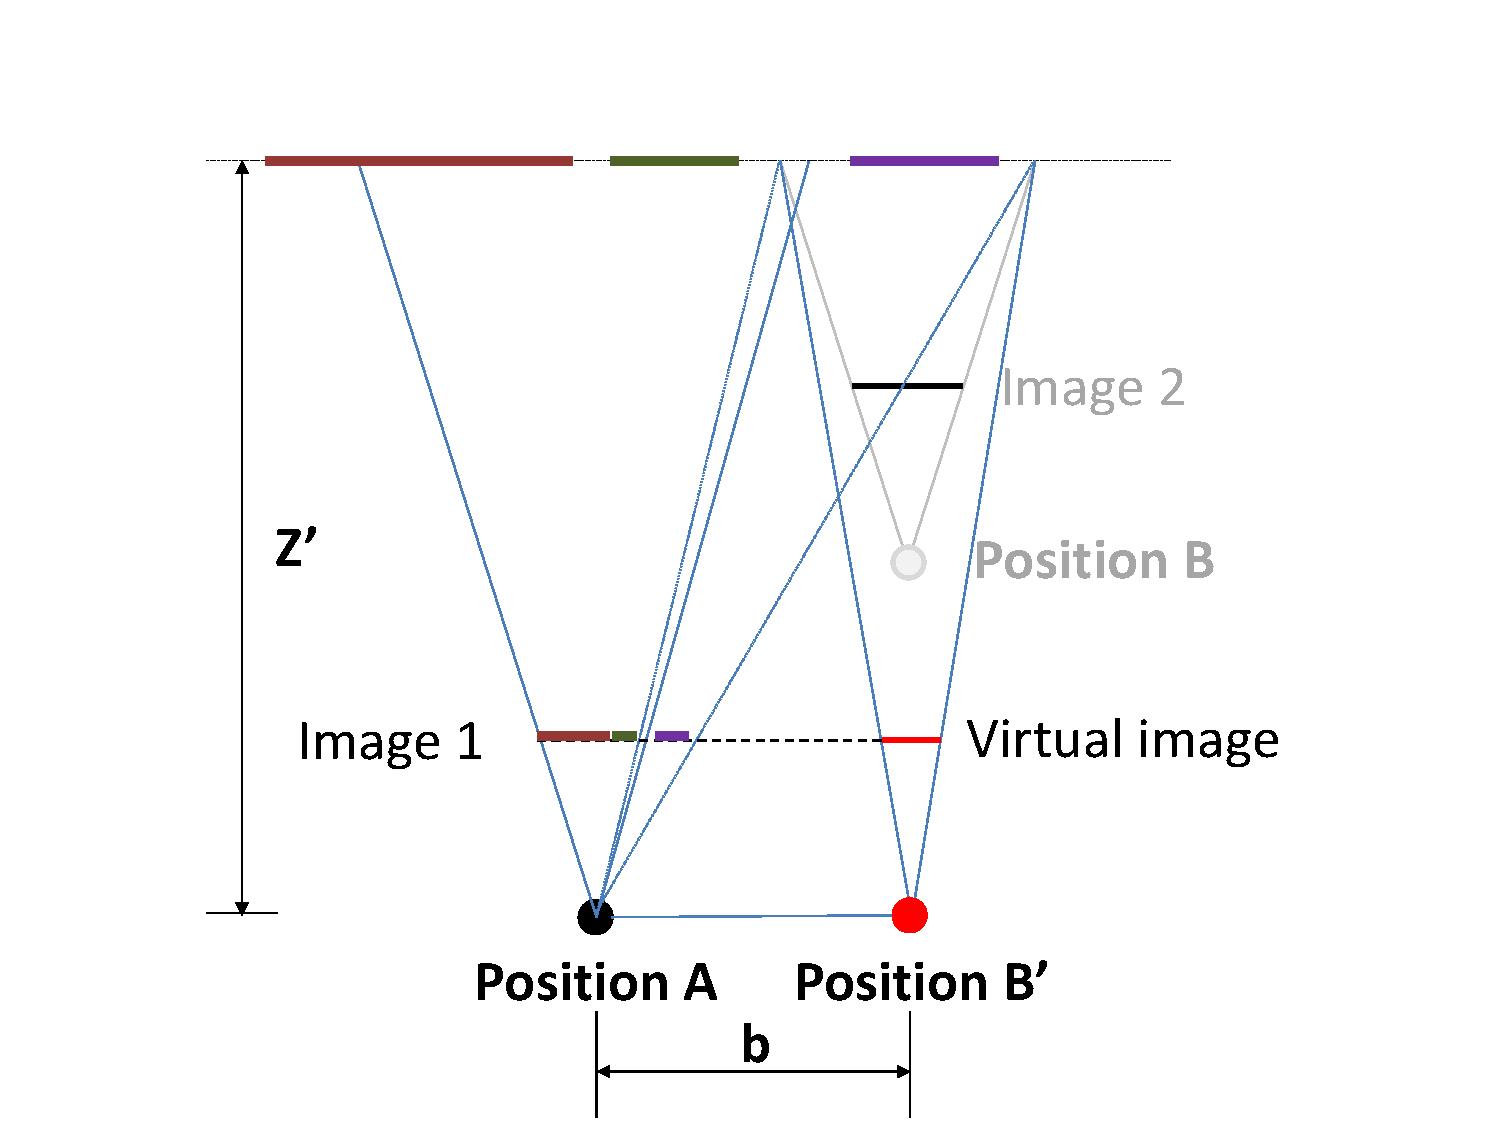
\includegraphics[width=0.8\textwidth]{figures/vacantSpaces/stereo} 
  \caption[Creation of Super-panoramas]{ \label{fig:stereo} (Top) The virtual
  picture as seen from position B' is computed using Equation~\ref{eq:moveRelation} from the real picture
    taken from B.  (Bottom) Using the stereo disparity, calculated from the baseline 
   width b and depth Z',  it is possible to depict the composite scene obtained from both A
  and B' (from the view point of A).}
\end{figure}    
Assume that a mini-panorama is created from these two areas, and the
depth of the planar surface from the camera is more for A, than for
B. We then take the mini-panorama image captured at B, and `move' it to
a new location B' whose depth (from the imaged surface) is the same as
that of A. The resulting image  will be smaller; the images are
related by the equation
\begin{equation}
  \label{eq:moveRelation}
  {\bf \frac{x'}{x} = \frac{Z}{Z'}}
\end{equation}
where {\bf x} (respectively {\bf x'}) represents a pixel location of
the image in B (respectively, B') and 
{\bf Z} (respectively {\bf Z'}) represents the depth of the images
surface from B (respectively, B').

In order to form a super-panorama from the depth of A, we can now
treat the resulting images from A (unchanged) and B’ (computed from
Equation~\ref{eq:moveRelation}) forming a simplistic stereo pair at
the depth of position A.  Using the stereo disparity formula we can
``place,'' from the view point of A, the image captured from B',
thereby creating a super-panorama. (We could as well present the
entire scene from the viewpoint of B' (since it is at the same depth);
we prefer these pictures to the one that one may be created from the
depth of B.)

% In theory, one may for the super-panorama from viewpoint B, by first
% moving position A to the same depth as of position B. But in that
% case, virtual image of A formed at the depth of position A will be
% ``zoomed-in'' version which may cause pixelization.

\begin{figure}[h]
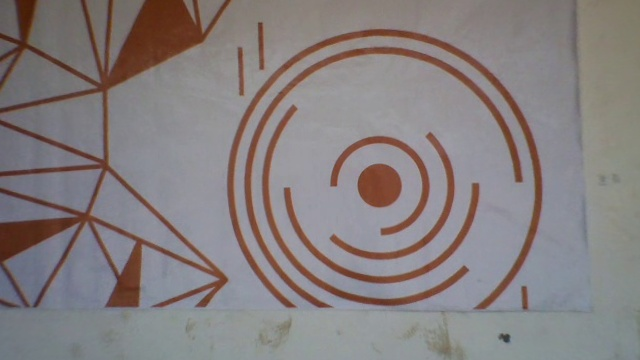
\includegraphics[width=0.48\textwidth]{images/left}

\includegraphics[width=0.48\textwidth]{images/right}
\caption[Example of super-panorama]{Candidate images for a super-panorama taken
from different depths. For context, see Fig.~\ref{fig:results}.  These images are
  `reference` images (spanning  tree center) of individual  mini-panoramas.}
\label{fig:exmaple}
\end{figure}

\textbf{Example:} Consider two images (shown in Fig.~\ref{fig:exmaple}) taken from the positions
(1.37, 0.85, 1.6), and (3.75, 0.98, 1.4).  As their depths are
different, we (virtually) move the second image by shrinking the
second image by a factor $\frac{1.4}{1.6}$, i.e., to 87\% of its
original size. With both images at the same depth (1.6m), the 
disparity of the second image is 
\begin{center}
$\text{disparity}_x = (3.75 - 1.37)f/1.6 = 839$\\
$\text{disparity}_y = (0.85 - 0.98)f/1.6 = -45$
\end{center}
where $f$ is focal length of the quadcopter camera in pixel units.

\subsection{Summary: Use of IMU}
The IMU data is used primarily for two purposes:
\begin{enumerate}
\item \textbf{Selection and ordering of images:} We use the IMU data
  to select representative images from the video and arrange them into
  rectangular grid according to the `spatial' neighborhood. It also
  disambiguates situations when multiple images that are spatially
  distant, but have similar, repeated features.

\item \textbf{Super-panorama:} Whenever there are no features in
  the overlap region of two images, we use the IMU data to find the
  relative position of one image w.r.t. second image as shown in the
  example. 
\end{enumerate}
\setlength{\tabcolsep}{2pt}
\section{Experiments and Results}
\label{sec:results}

All our experiments have been completed with the inexpensive consumer
quadcopter called a Parrot's AR Drone 2.0. The imagery acquired were
from actual graffiti painted on large walls as well as posters in an
exhibition.  We have used the ROS based ARDrone Autonomy
Driver to communicate with the drone. For the purpose of showing the
efficacy of our method, we also took a picture of the scene from a
distance with a smartphone camera to better understand the scene.

We have implemented our algorithm in C++ using the OpenCV library
(OpenCV 2.4.9). Experiments were performed on a PC with Intel Core i7
processor(@3.4GHz) and 8GB RAM.  
%The source code to produce
%interesting images from a video, and to generate the super-panorama,
%as well as the data sets used in this paper will be made publicly
%available after acceptance of the paper.

\subsection{Selecting Images}

In our first experiment, we wanted to ensure that the selection of
images done was comprehensive and useful.  We sent the drone to image 
an outdoor scene with no vacant space. This experiment was conducted
in an outdoor environment. We note here that there were approximately
3000 images in the raw video.  AutoStitch and Photoshop were unable to 
cope  when fed with this large number of frames.

One way to produce some sort of mosaic was to simply reduce the amount
of data given to AutoStitch.  Figure~\ref{fig:sac3}(a) shows uniformly
(time) sampled images from the video.  When these sampled images are
given to AutoStitch or to Adobe Photoshop, we find
(Figure~\ref{fig:sac3}(b)) that these programs are able to produce
some output, but the results are not satisfactory.

Instead of feeding time-sampled images, we ran our albumization
algorithm (as explained in Section~\ref{sec:selection}) on the video
which resulted in $N = 5$ images.  Though the number of input images
in the video is large, the total distance covered by the quadcopter in
this duration (of around 90 seconds) is small; thus the
number of distinct images returned by the algorithm shows a dramatic
reduction. Figure~\ref{fig:sac3}(c) shows examples of selected images.
Many of the images are similar to the time sampled version; however,
the occasional differences are enough to make AutoStitch work. The
results are shown in Figure~\ref{fig:sac3}(d).


\begin{figure}[hb!]
\centering
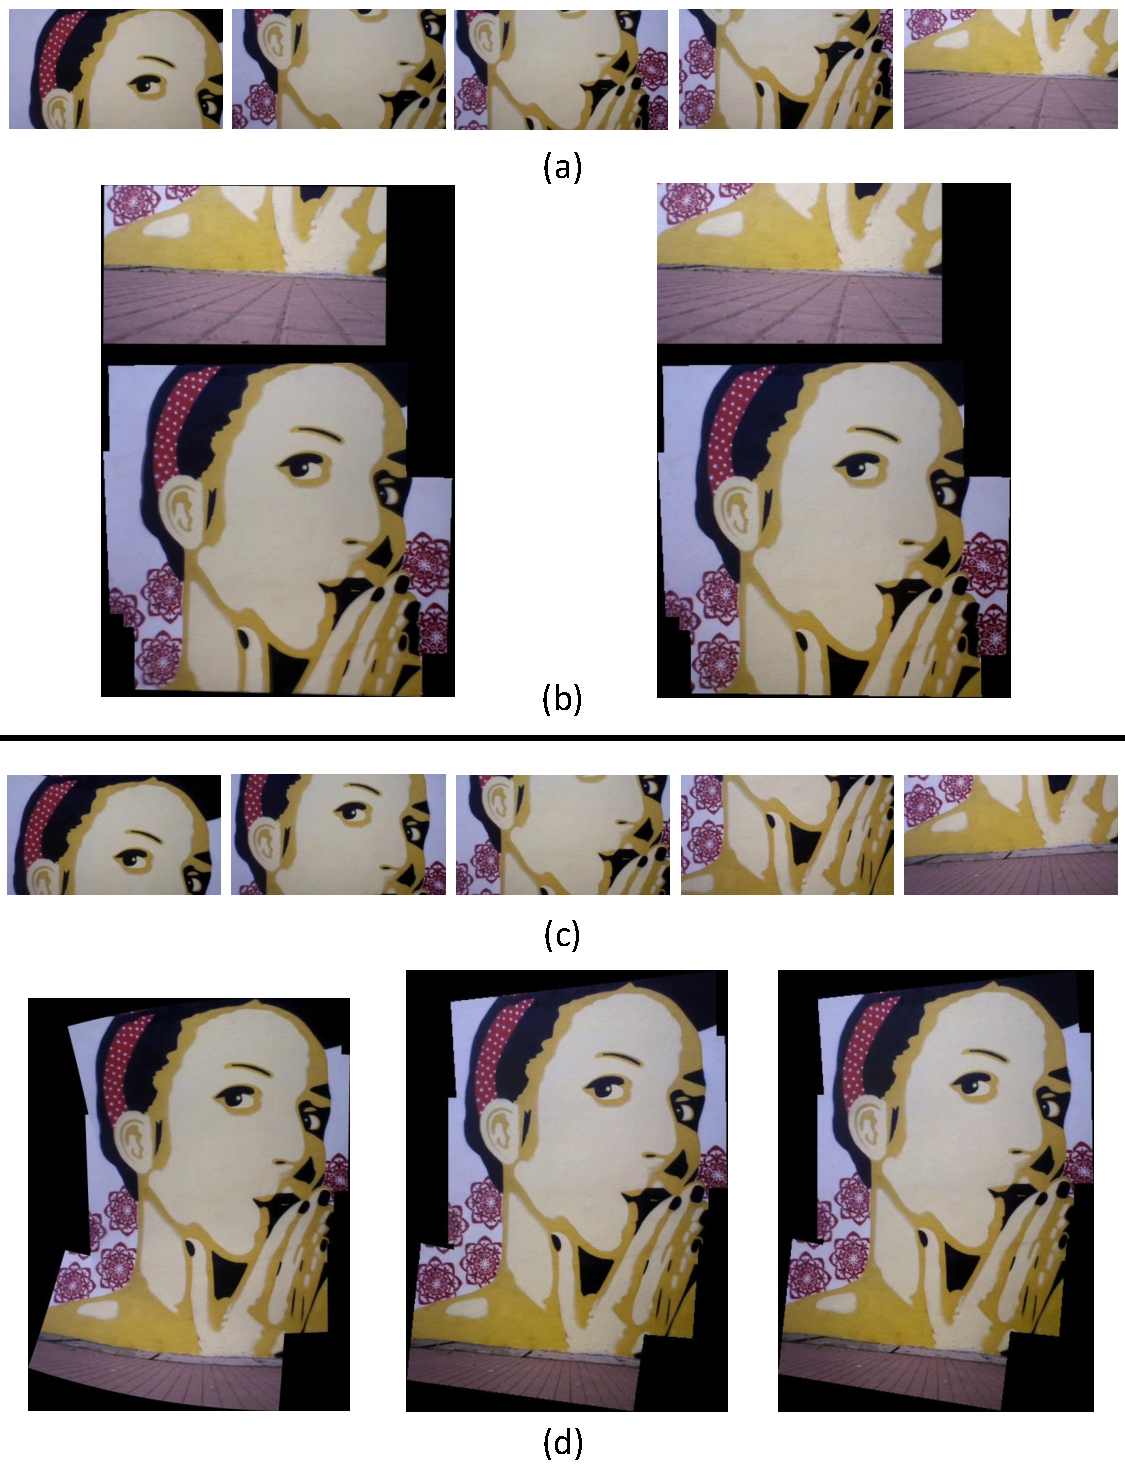
\includegraphics[width=0.87\linewidth]{figures/vacantSpaces/ValidationResult}
\caption[Validation Result: Lady]{ (a) Uniformly sampled images from an outdoor
video expedition.  (b) Output of the state of the art photo stitchers
  (left:AutoStitch, right:Adobe Photoshop CS6) on uniformly time
  sampled images.  As time sampled images do not guarantee coverage of
  the scene, the panorama is broken. The top portions do not belong at
  the right place (see (d)) (c) Salient image selection from the set of
  approximately 3000 images using positional information. (d) When
  salient images are given to AutoStitch (left) and Photoshop (middle),
  we can create a panoramic mosaic (since there are no vacant
  spaces). We also show the result from our stitching algorithm
  (bottom right).}
\label{fig:sac3}
\end{figure}

In summary, this experiment provides evidence to show that (a) our
albumization algorithm is reasonable and (b) our stitching
results are comparable to that of AutoStitch for the kind of scenes
considered.

\subsection{Indoor Imagery with Vacant Spaces}

Our next selection of experiments were conducted in an indoor
environment.  

The input stream had about 4300
images. The selection algorithm (Section~\ref{sec:selection}) pruned the video
into $N=5$ images. A sample of the selected images are seen in Figure~\ref{fig:vacantTeaser}.

There were two disconnected components in the resulting graph.
AutoStitch was unable to produce any reasonable output as seen in
Figure~\ref{fig:vacantTeaser}.  The scene, captured from a distance is also
shown.  One can see a better orthographic view of the posters.

\textbf{Cars:}
In an another experiment, the input stream had about 9000 input
images.  The selection algorithm (Section~\ref{sec:selection}) pruned
the video into $N=13$ images. A sample of the selected images are seen
in Figure~\ref{fig:indoor_results}(a).  The scene as captured by a
smartphone can also be seen, as well as the outputs of the state of
the art stitchers. Note that AutoStitch is only able to stitch the
upper half of the scene.  Our result
Figure~\ref{fig:indoor_results}(e) clearly stands out in comparison.

\begin{figure}
\centering
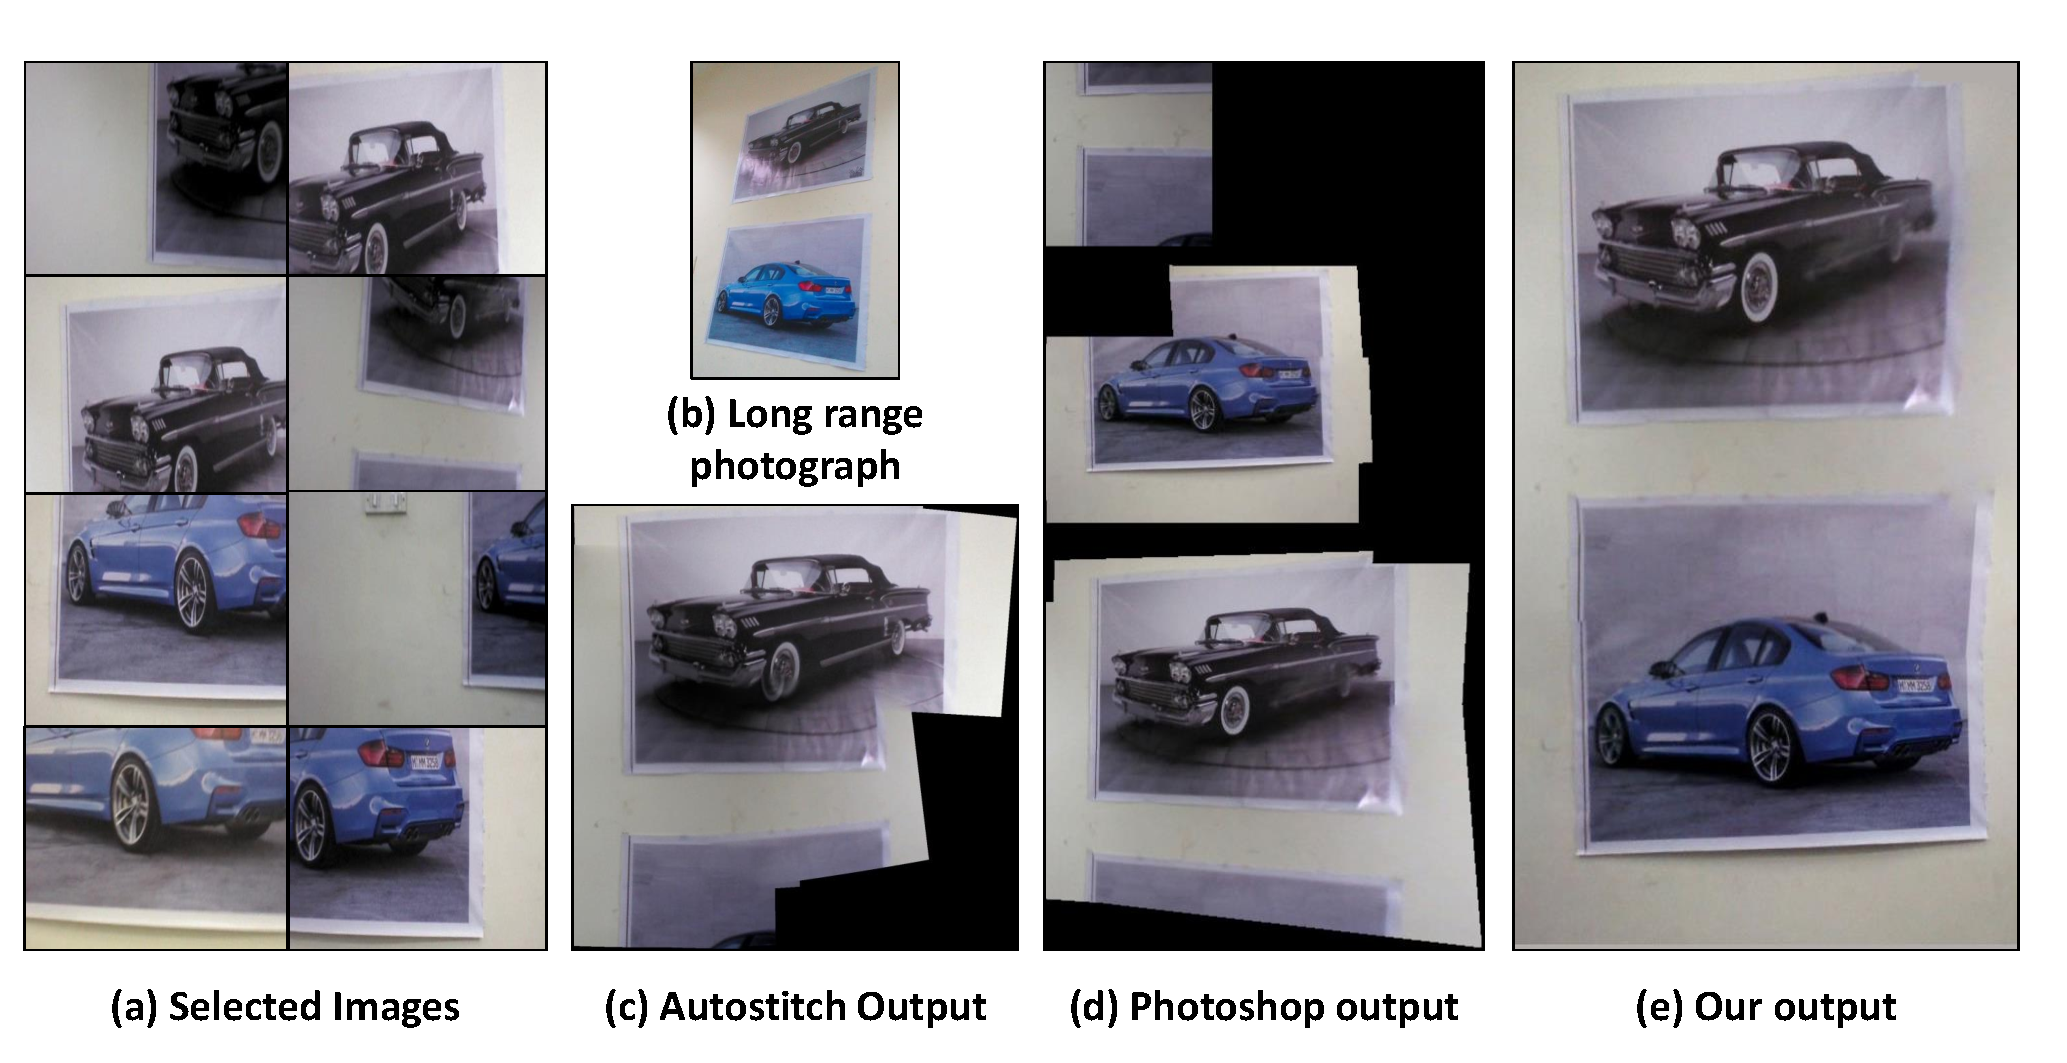
\includegraphics[width=\linewidth]{figures/vacantSpaces/indoor_results}
\caption[Result: Cars]{ (a) Pruned images from the quadcopter video using our
  saliency algorithm of (b) an indoor scene. This long range photograph
  has been captured separately by a smartphone camera only for
  context. Notice a significant vacant space in the imagery.  (c)
  Output of AutoStitch -- only the upper half of the scene is output.
  (d) Output of Adobe Photoshop CS6 -- the vacant space posed a problem to the
  feature matching algorithm, so instead of a mosaic, individual
  pieces were output as mini-panoramas (e) Our output on the selected
  images. We are able to present the scene in high fidelity in an
  orthographic view.}
\label{fig:indoor_results}
\end{figure}

\textbf{Aircrafts 1:} The input stream had about 9100 images. The selection
algorithm pruned the video into $N=14$ images. The scene as captured by a
smartphone can also be seen in Figure~\ref{fig:aircrafts1}(b). A sample of the
selected images are seen in Figure~\ref{fig:aircrafts1}(a).
Figure~\ref{fig:aircrafts1}(c,d,e) shows the comparison of outputs of state of
the art stitchers with the output of our algorithm. As there are vacant spaces,
AutoStitch~\cite{autostitch} is able to join only top part of the scene, while
Photoshop~\cite{photoshop} is showing two disconnected components.
In contrast, since we use positional data, our output is an acceptable mosaic,
and shows an orthographic view.

\begin{figure*}[h!]
	\centering
	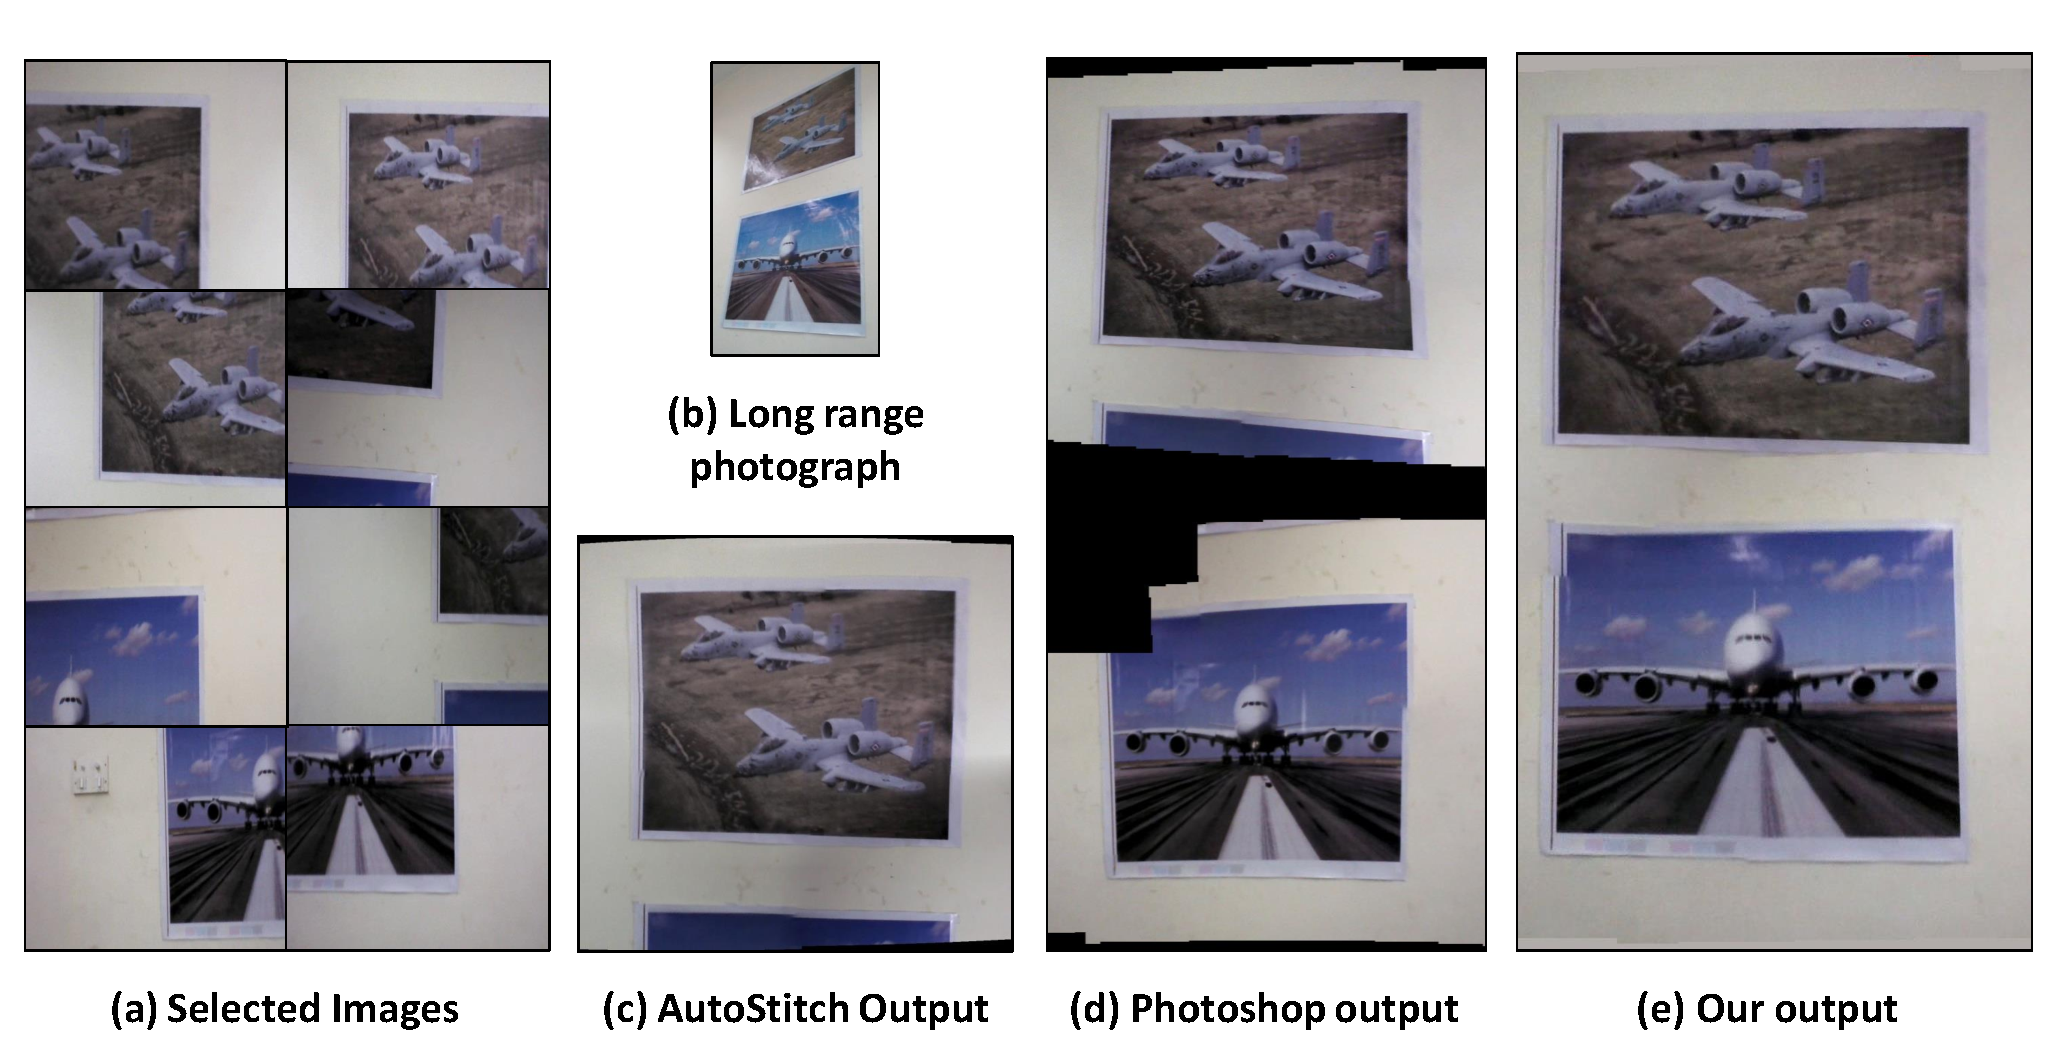
\includegraphics[width=\linewidth]{figures/vacantSpaces/aircrafts1}
	\caption[Result: Aircrafts]{(a) Pruned images from the quadcopter video using
	our saliency algorithm of (b) an indoor scene. This long range photograph has been captured separately by a smartphone camera only for context. Notice a significant vacant
space in the imagery. (c) Output of AutoStitch - only the upper half of the scene is output. (d) Output of Adobe Photoshop CS6 - 
the vacant space posed a problem to the feature matching algorithm, so instead of a mosaic, individual pieces were output as mini-panoramas (e) Our output on the
selected images. We are able to present the scene in high fidelity in an orthographic view.}
	\label{fig:aircrafts1}
\end{figure*}

\subsection{Outdoor Imagery with Vacant Spaces}

\begin{figure}[h!]
\centering
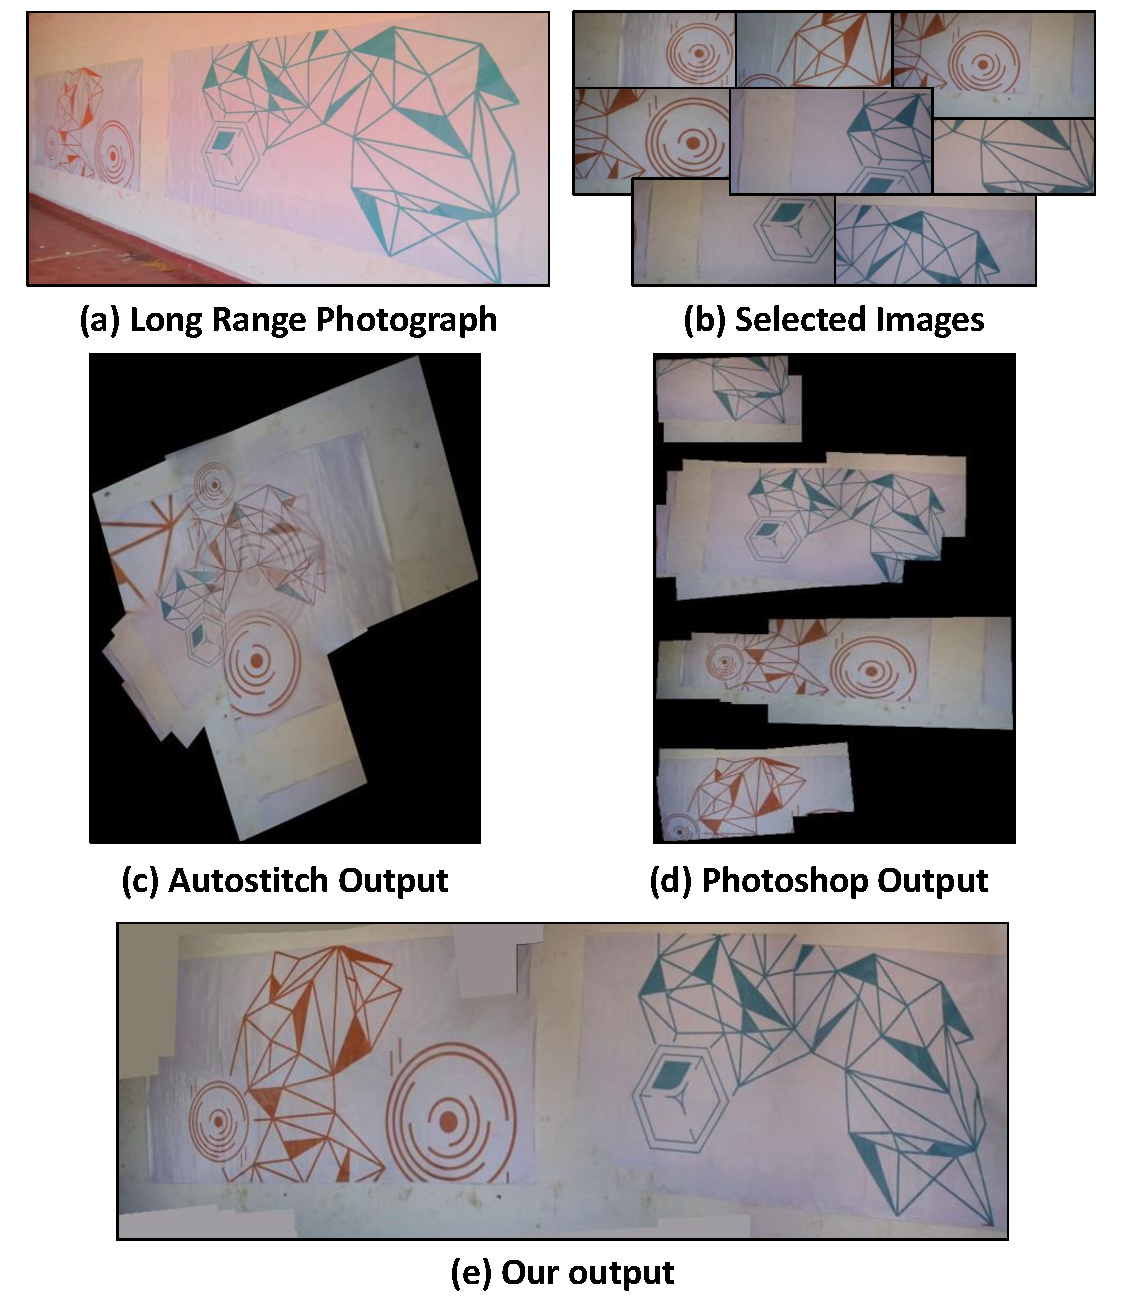
\includegraphics[width=\linewidth]{figures/vacantSpaces/orange_blue}
\caption[Result: Outdoor Exhibition]{(a) An outdoor scene captured by a standard
camera in an exhibition. The approach to the area is normally cordoned off and one
  needs permission to get a quadcopter to take the picture.  Notice a
  significant gap between the two posters.  (b) Pruned images from the
  quadcopter video using our saliency algorithm. (c) Output of
  AutoStitch on the selected images. The mosaic is not reasonable
  presumably because of the confusion in features. (d) Output of Adobe
  Photoshop CS6 on the selected images. The vacant space posed a
  problem to the feature matching algorithm, so instead of a mosaic,
  individual pieces were output as mini-panoramas (e) Our output on
  the selected images. We are able to join two posters (separated by
  vacant space) using the IMU data.}
\label{fig:results}
\end{figure}

Our next set of experiments were conducted in an outdoor
environment. The input stream had about 12000 images. The selection
algorithm pruned the video into $N=30$ images. A sample of the
selected images are seen in Figure~\ref{fig:results}(a).  The scene as
captured by a smartphone can be seen in Figure~\ref{fig:results}(b).
Figures~\ref{fig:results}(c), (d) and (e) shows the comparison of outputs of
state of the art stitchers with the output of our algorithm. Note that
AutoStitch is getting confused by too many matching features. 
Please see supplementary material for results on other indoor as well as outdoor datasets.

Figure \ref{fig:results2} shows comparison of outputs of state of the art
stitchers with output of our algorithm on another dataset.

\begin{figure}[h!]
\centering
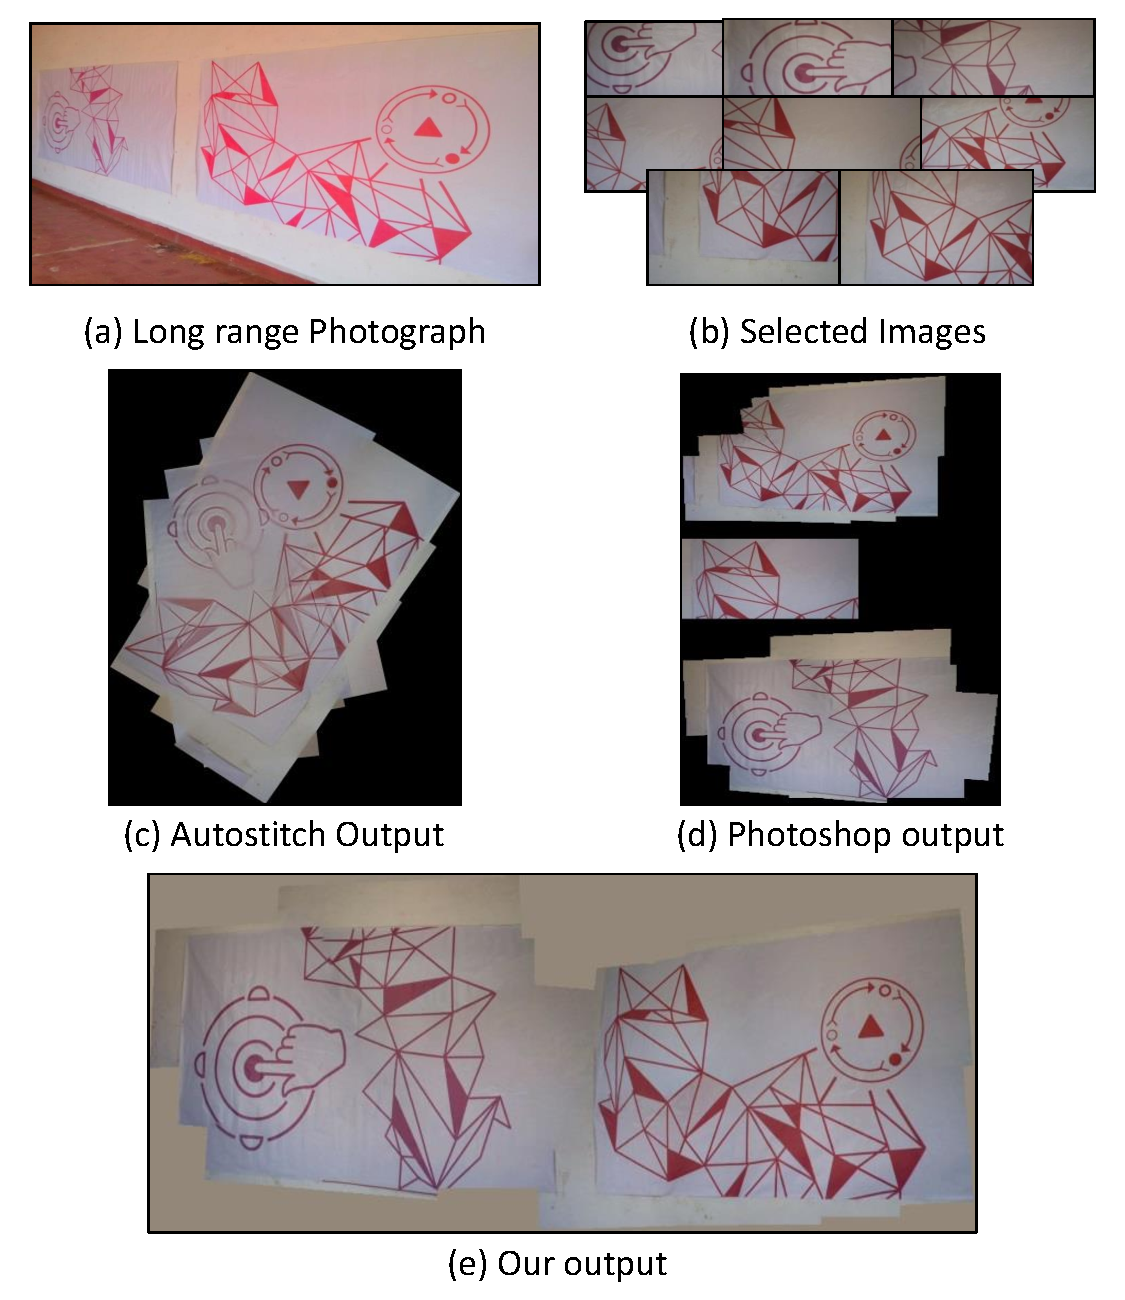
\includegraphics[width=\linewidth]{figures/vacantSpaces/Purple_red} 
\caption[Result: Outdoor
Exhibition 2]{(a) Another outdoor
scene captured by a standard camera in an exhibition. The approach to the area is normally cordoned off and one
  needs permission to get a quadcopter to take the picture.  Notice a
  significant gap between the two posters.  (b) Pruned images from the
  quadcopter video using our saliency algorithm. (c) Output of
  AutoStitch on the selected images. The mosaic is not reasonable
  presumably because of the confusion in features. (d) Output of Adobe
  Photoshop CS6 on the selected images. The vacant space posed a
  problem to the feature matching algorithm, so instead of a mosaic,
  individual pieces were output as mini-panoramas (e) Our output on
  the selected images. We are able to join two posters (separated by
  vacant space) using IMU data.}
\label{fig:results2}
\end{figure}


\subsection{Analysis}

The performance of our algorithm as a function of the scene, as well
comparison with other software is summarized in
Table~\ref{tbl:results}.  It can be seen that, whenever there is
vacant spaces between adjacent images, AutoStitch produces only
one component, presumably the largest.  Adobe Photoshop outputs all disconnected
components. Sometimes due to the lack of spatial proximity
information, the resulting images (or components) are disconnected instead of being 
mosaiced (unlike AutoStitch). In contrast, in all cases, our algorithm
successfully uses proximity information which results in a reduced number of mini-panoramas. 

As expected the number of selected images in our saliency algorithm
varies based on environment considerations (outdoor/indoor), the
average depth from the scene, and the total scene area.
 
\begin{table*}
\scriptsize

\newcolumntype{C}{ >{\centering\arraybackslash} m{1.1cm} }
\newcolumntype{D}{ >{\centering\arraybackslash} m{1.5cm} }

\begin{tabular}{|C|C|C|C|D|D|D|m{6.5cm}|}
\hline
Dataset 
& Number of Images in video 
& Approx. planar area covered
& Number of selected images 
& AutoStitch: \# Components 
& Photoshop: \# Components
& Our algorithm: \#mini- panoramas
& \multicolumn{1}{p{6.5cm}|}{\centering Remarks}\\
\hline

\hyperref[fig:sac3]{Lady} & 3000 & 60 sqft. & 5 & 1 & 1 & 1 & As there are enough features
in the intersection of selected images, AutoStitch, Photoshop as well
as our algorithm produces the  panorama correctly.\\\hline
%Spray Woman} & 9000 & 70 sqft. & 15 & 1 &
%1 & 1 & As there are enough features in the intersection of selected images,
%AutoStitch, Photoshop as well as our algorithm gives full panorama
%correctly. As this scene was captured nearer from the plane than
%earlier, we need to select more images than earlier dataset.\\\hline 

\hyperref[fig:vacantTeaser]{Indoor exhibition} & 4300 & 40 sqft. & 5 &
1 & 2 & 2 & As there is vacant space between the two posters,
AutoStitch produces only one panoramic image. Photoshop outputs two
posters as two disconnected components; these correspond to our mini-panoramas.
\\\hline 

\hyperref[fig:indoor_results]{Cars} & 9000 & 60 sqft. & 13 & 1 & 3 & 3 &
As there is vacant space between the two visuals, AutoStitch produces
only one panoramic image, the black vehicle.  In the case of
Photoshop, two of the three disconnected 
components represents two partial visuals, while the third component is
the intersection  between the two cars -- this portion contains featureless
space.\\\hline

\hyperref[fig:results]{Outdoor exhibition} & 12000 & 80 sqft. &
30 & 1 & 4 & 2 &  AutoStitch is confused by the replicated features in
the two posters which are sometimes proximal and sometimes
geographically distant.  A single panorama is produced, but the output
is incorrect. We use the IMU data
for arranging the images in spatial neighborhood; we have fewer
mini-panoramas.  Photoshop is not able to produce a super-panorama and
the number of disconnected components in Photoshop's output is larger
than the number of mini-panoramas.\\\hline  
\end{tabular}
\caption{Quantitative summary of  results.}
\label{tbl:results}
\end{table*}



\section{Concluding remarks}

In this chapter, we have described a method of imaging large scenes
using a quadcopter enabling close orthographic views. We also defined
a new problem, that of computing a mosaic of a planar scene with
vacant spaces.  Vacant space relates to images in an input stream
where there are not enough features for traditional mosaicing
algorithms to estimate geometric warps to align the images.

Our solution to this problem is to use an autonomous quadcopter which
is capable of taking pictures.  The quadcopter has an inertial
measurement unit that is capable of outputting approximate
positions. Using this positional information, our algorithm selects an
``interesting'' subset of the video imagery.  This subset consists of
pictures taken with a moving camera; we reduce the resulting
problem of computing a mosaic by reduction to the stereo problem.  Our
method works on both indoor and outdoor scenes.

Controlling a consumer-focused inexpensive quadcopter can be
problematic; for instance the quadcopter could have severe yaw and
roll.  For future work, vision based algorithms to control such
quadcopters might be quite useful.
\chapter[Multiplanar Imaging]{Autonomous Imaging of Multiplanar Regions through
Quadcopter}
\label{ch:multiplanar}
\section{Introduction}
Consider a visit to the art gallery or a tour to ancient temples for restoration. In
such scenarios, we would like to get an unrolled view of scenes depicted on
the walls. We need to capture each surface orthographically from close range to
get minute details required for further work. We may use SLR cameras or even
smartphones having high-resolution cameras which are easily available for
imaging such scenes. Many of these cameras also have special modes to capture
panoramas.
\begin{figure}[h!]
\centering
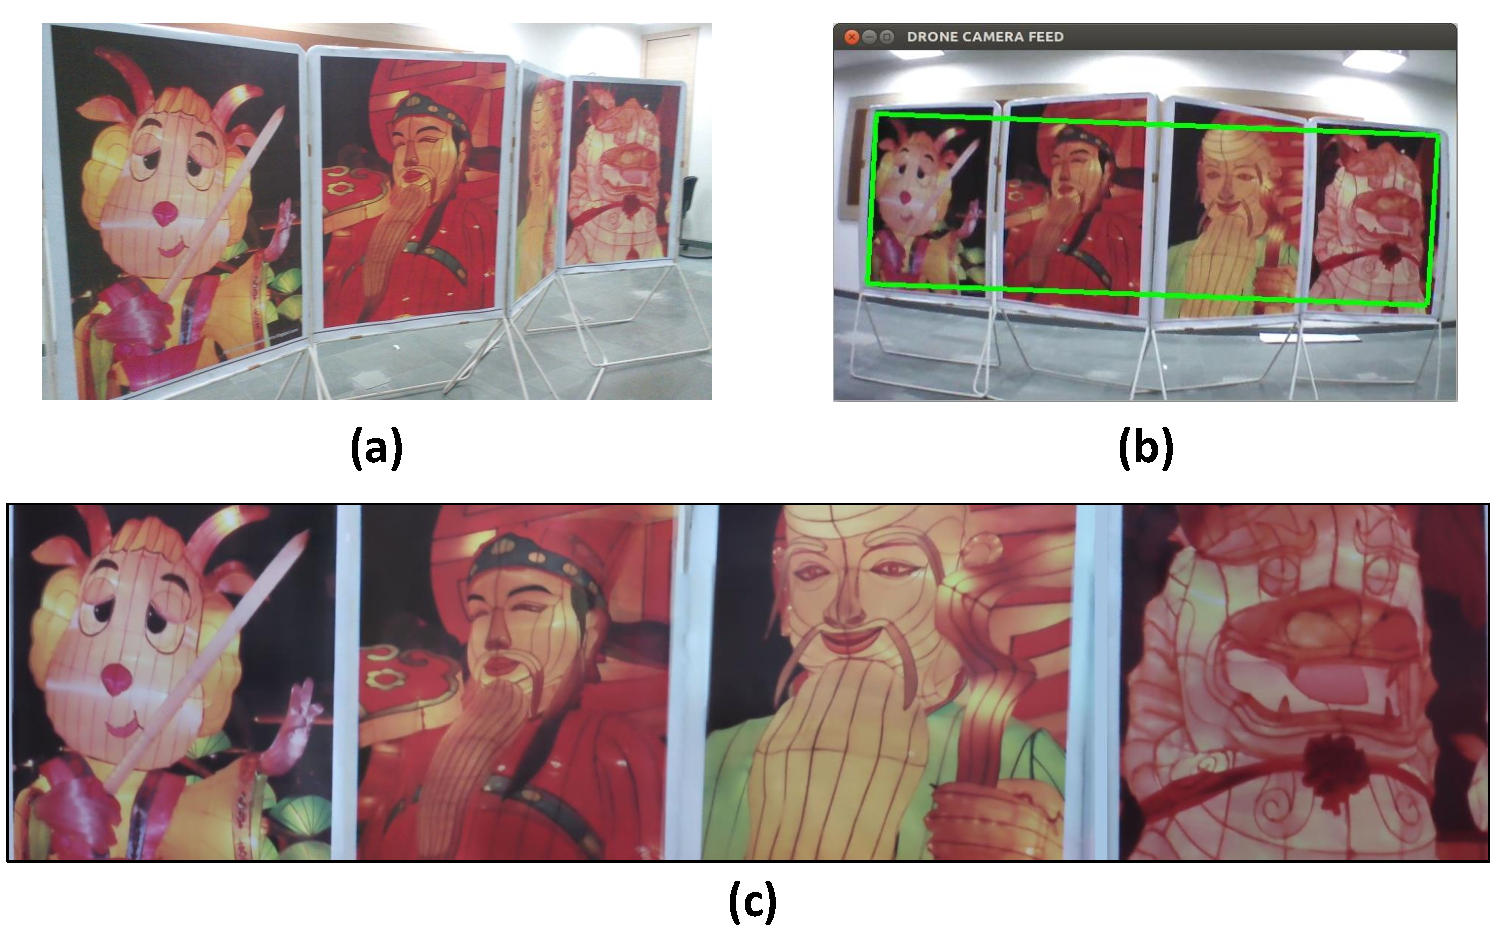
\includegraphics[width=0.98\linewidth]{figures/multiplanar/teaser2}
\caption[Overview of multiplanar imaging]{The multiplanar scene to be mosaiced
is shown in (a).
Long range photograph doesn't give details of all images. The quadcopter has to be moved back
to allow the user to select the area of interest as shown in (b).
Final mosaicing output from this paper is shown in (c). Size of our output is
3427 x 863 pixels.}
\label{fig:teaser}
\end{figure} 

\begin{figure}[htb]
\centering
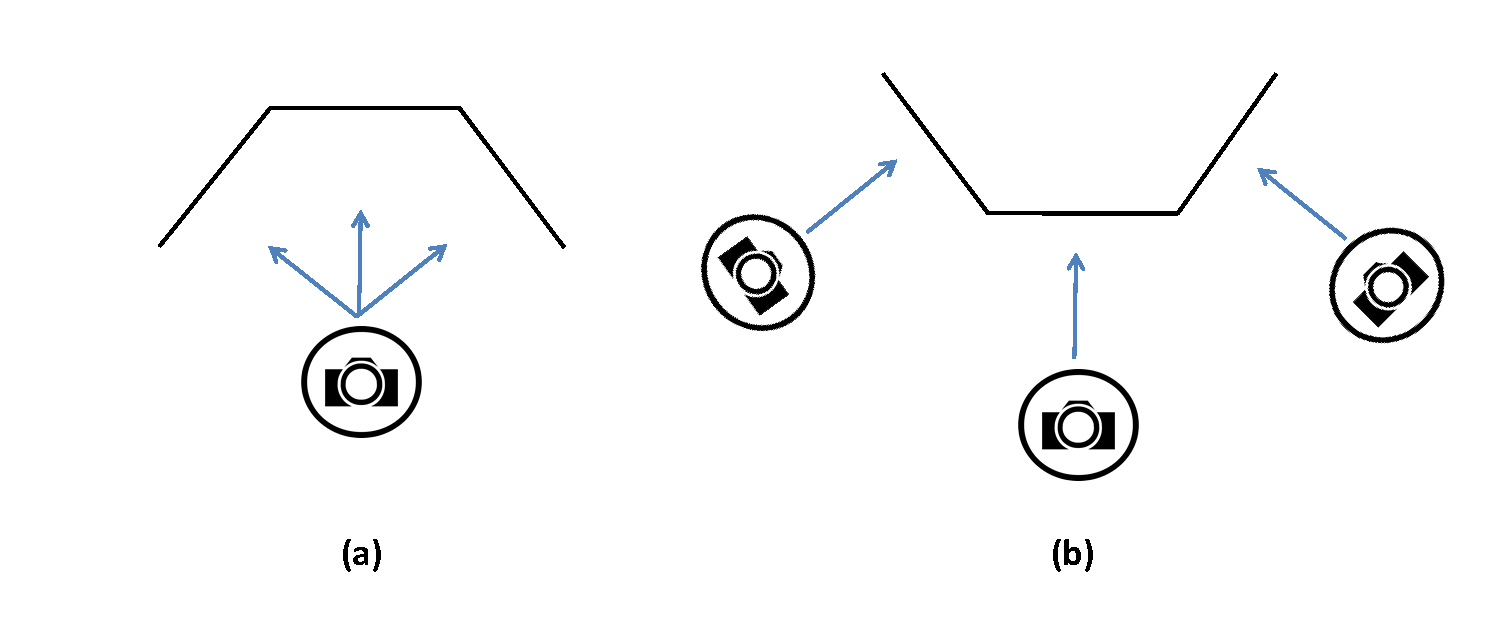
\includegraphics[width=\textwidth]{figures/multiplanar/ConcaveConvex}
\caption[Imaging concave surfaces versus convex surfaces ]{(a) Imaging concave
surfaces. We do not have to change our position, changing orientation is
sufficient to capture the whole surface. (b) While imaging convex surface, one
need to change the position as well as the viewing angle. It makes the process
of building homography based panorama  theoretically impossible.}
\label{fig:convex_concave}
\end{figure}

But practically, when we use such cameras for capturing panoramas, we do not
get the close-up orthographic view of the scenes present at height or not
easily accessible. We also need a steady hand for a long time while capturing
panoramas which might be too tiring.

The limitation of even an expensive SLR cameras is that it can create a panorama with
an orthographic view, only if the surface to be imaged is present on a single
plane. If the surface is concave and the camera is kept at the center of the
surface, only then we get panorama with an orthographic view (Figure
\ref{fig:convex_concave}(a)). But if the surface (or part of it) is convex (Figure \ref{fig:convex_concave}(b),
 viewpoint (along with the orientation) needs to be changed while imaging which
 prohibits the use of panorama mode of most cameras. Even if any camera allows such panorama creation, the output
is distorted due to change in homography. 

In scenarios where handheld devices cannot capture orthographic view of the
input scene, or if the scene is too large, an inexpensive flying device such as
a quadcopter can be used. A quadcopter can cover any large scene with
an orthographic view with precise details (e.g., facial features of a person in
Figure \ref{fig:teaser}) by flying in front of each part of the scene.
Even if we use a quadcopter, manually controlling the quadcopter to image a
large scene spread over multiple planes is a tedious task and hence require
automation.

\textbf{Problem Definition}
In \cite{Prasad16},  an imaging application with the use of a quadcopter is
developed. It handles large scenes and scenes with featureless (vacant) spaces.
%But a few things were not considered in \cite{Prasad16}.%
%The first one is regarding navigation and control of quadcopter.%
We found that manually navigating the quadcopter is a very laborious process.
Also, we may not be able to cover the user specified area if we are controlling
quadcopter through a keyboard or joystick controller.

Also in \cite{Prasad16}, the mosaicing algorithm could
mosaic only if the scene lies on a single planar surface. But the real world is 
made of a multiplanar surface. In fact, we have many circumstances where the
input scene is spread over multiple planes. In such cases, we would like to
image each planar region orthographically and then `unroll' the whole scene by joining the
individual mosaics so that we get the output mosaic of the input scene as if it
is present on a single plane.
 
\textbf{Challenges}
We need to autonomously navigate quadcopter to capture the whole scene. Generally
Global Positioning System (GPS) is used for navigation of UAVs.
But GPS does not work effectively and precisely in indoor scenarios. Even in outdoor
scenario we may not rely fully on GPS due to various reasons such as GPS
jammer, spurious signal, etc.. Hence, we need a reliable navigation system to
maneuver the quadcopter in an unknown environment.

A quadcopter has onboard an IMU (Inertial Measurement Unit)  which consists of
accelerometers, gyroscopes, and magnetometers. The IMU provides pose which can be
used to   determine desired locations from where the whole scene can be covered.
Due to the  jerky nature of an inexpensive quadcopter, the IMU sometimes
provides erroneous measurements  which result in incorrect pose information. There comes need of
further calibration.  To provide quadcopter it’s precise coordinates we need
some application which can do a real-time calibration.
A technique named Parallel Tracking and Mapping(PTAM) \cite{klein} is introduced
to estimate camera pose in an unknown scenario.
Engel et al. \cite{engel} have used both PTAM and IMU data to estimate  correct
positional information.

The quadcopter can cover the given area of interest by the user reliably using pose
estimates given by method in \cite{engel}. But even a three-minute video
captured by quadcopter, resulting in thousands of images overwhelm any mosaicing
application. Here instead of videographing the whole area, quadcopter should
hover at certain points to take images such that whole scene can be covered with
minimum images. For this, we need an algorithm which calculates those
specific positions  where quadcopter is hovered and records HD video to give
full mosaic.

In the case of multiplanar surfaces, these problems worsen. In the case of concave
surfaces (Figure \ref{fig:convex_concave}(a)) if the camera is placed at the
center of concave surface, imaging can be done from the single viewpoint.
But if the plane is convex(Figure \ref{fig:convex_concave}(b)), viewpoints need
to be changed with different angles. The quadcopter has to recognize multiple planes
in real-time and then change its direction for every plane before imaging the
region so that it becomes normal to the plane.

Though \cite{engel} gives accurate positional information, the roll and
pitch information is not reliable due to jerky motion of quadcopter.
Additionally, 3D map output by \cite{engel} is an approximate sparse map of the
environment where some 3D points from the map may not be present in the real
scene. Hence, we cannot use only 3D map to reconstruct the 3D world of input
scene. Homography-based stitching  is more stable than 3D map building. So we
may use homography-based stitching for  mosaicing individual planar regions and then
use plane information and camera positions to join those mosaics to get
the unrolled view of the input scene.

\textbf{Contributions}
Our goal is to image multiplanar region autonomously using a quadcopter. Initially,
3D positions of feature points on the imaging surface are estimated using PTAM
based method. These positions are used to detect multiple planes in real-time
using J-linkage. Then we ask the user to select the desired area spread over
multiple planes. Next positions of quadcopter for covering the user specified
area are calculated. These positions are such that user specified area is
covered with minimum images. 

Next, we fly the quadcopter orthographically to each plane and maneuver on
the planned path comprised of estimated positions (calculated in the earlier step).
The quadcopter is hovered for a small duration at each position to capture a video of a
part of the whole scene. Images from each plane are individually stitched together
using feature based homography, i.e., we get individual mosaics per plane. Finally, we join
individual mosaics using positional information from the quadcopter to give the
full mosaic.

The use of moving quadcopter for covering multiplanar surface may intrigue use
of Structure from Motion (SfM) paradigm. But SfM provides a sparse 3D map if
there are insufficient number of feature points (as well as correspondences).
Also, if we do texture mapping on the sparse 3D map output is not satisfactory.
Instead, we use homography based stitching to mosaic individual planes and merge
them to get unrolled view which is more effective than the sparse 3D map.


%Another minor problem with earlier method was: the quality of images. We were
%using images streamed over Wi-Fi channel which are of lesser size ($640 \times
%360$) than the size of images quadcopter stores on USB drive onboard i.e.,
%$1280 \times 720$. So, the quality of output mosaic would also be lesser. If we
%could synchronize the images stored on USB drive with the images streamed over
%Wi-Fi channel we could possibly get higher quality mosaic.

%The goal of this paper is to develop a method for autonomous control and
%navigation of quadcopter to cover the scene on a multiplanar surface. We also
%aim to provide unrolled view of a scene spread over multiplanar surfaces.



\section{Methodology}
The method adopted is pictorially depicted in the overview shown in Figure
\ref{fig:workflow} and is described in detail later on. In brief, we probe the
input scene through a quadcopter, calculate the 3D positions of feature points,
and detect multiplanar bounded regions from the area marked by the user through
our user interface. Path planning is done for each planar bounded region to find out
the camera positions. The quadcopter is autonomously maneuvered along the
estimated path and videos are captured at target points. For each planar
bounded region, the appropriate frame from each video is found and then given
to a mosaicing algorithm.  Finally, all mosaics are joined together to get a full
unrolled view.

\begin{figure}[ht!]
\centering
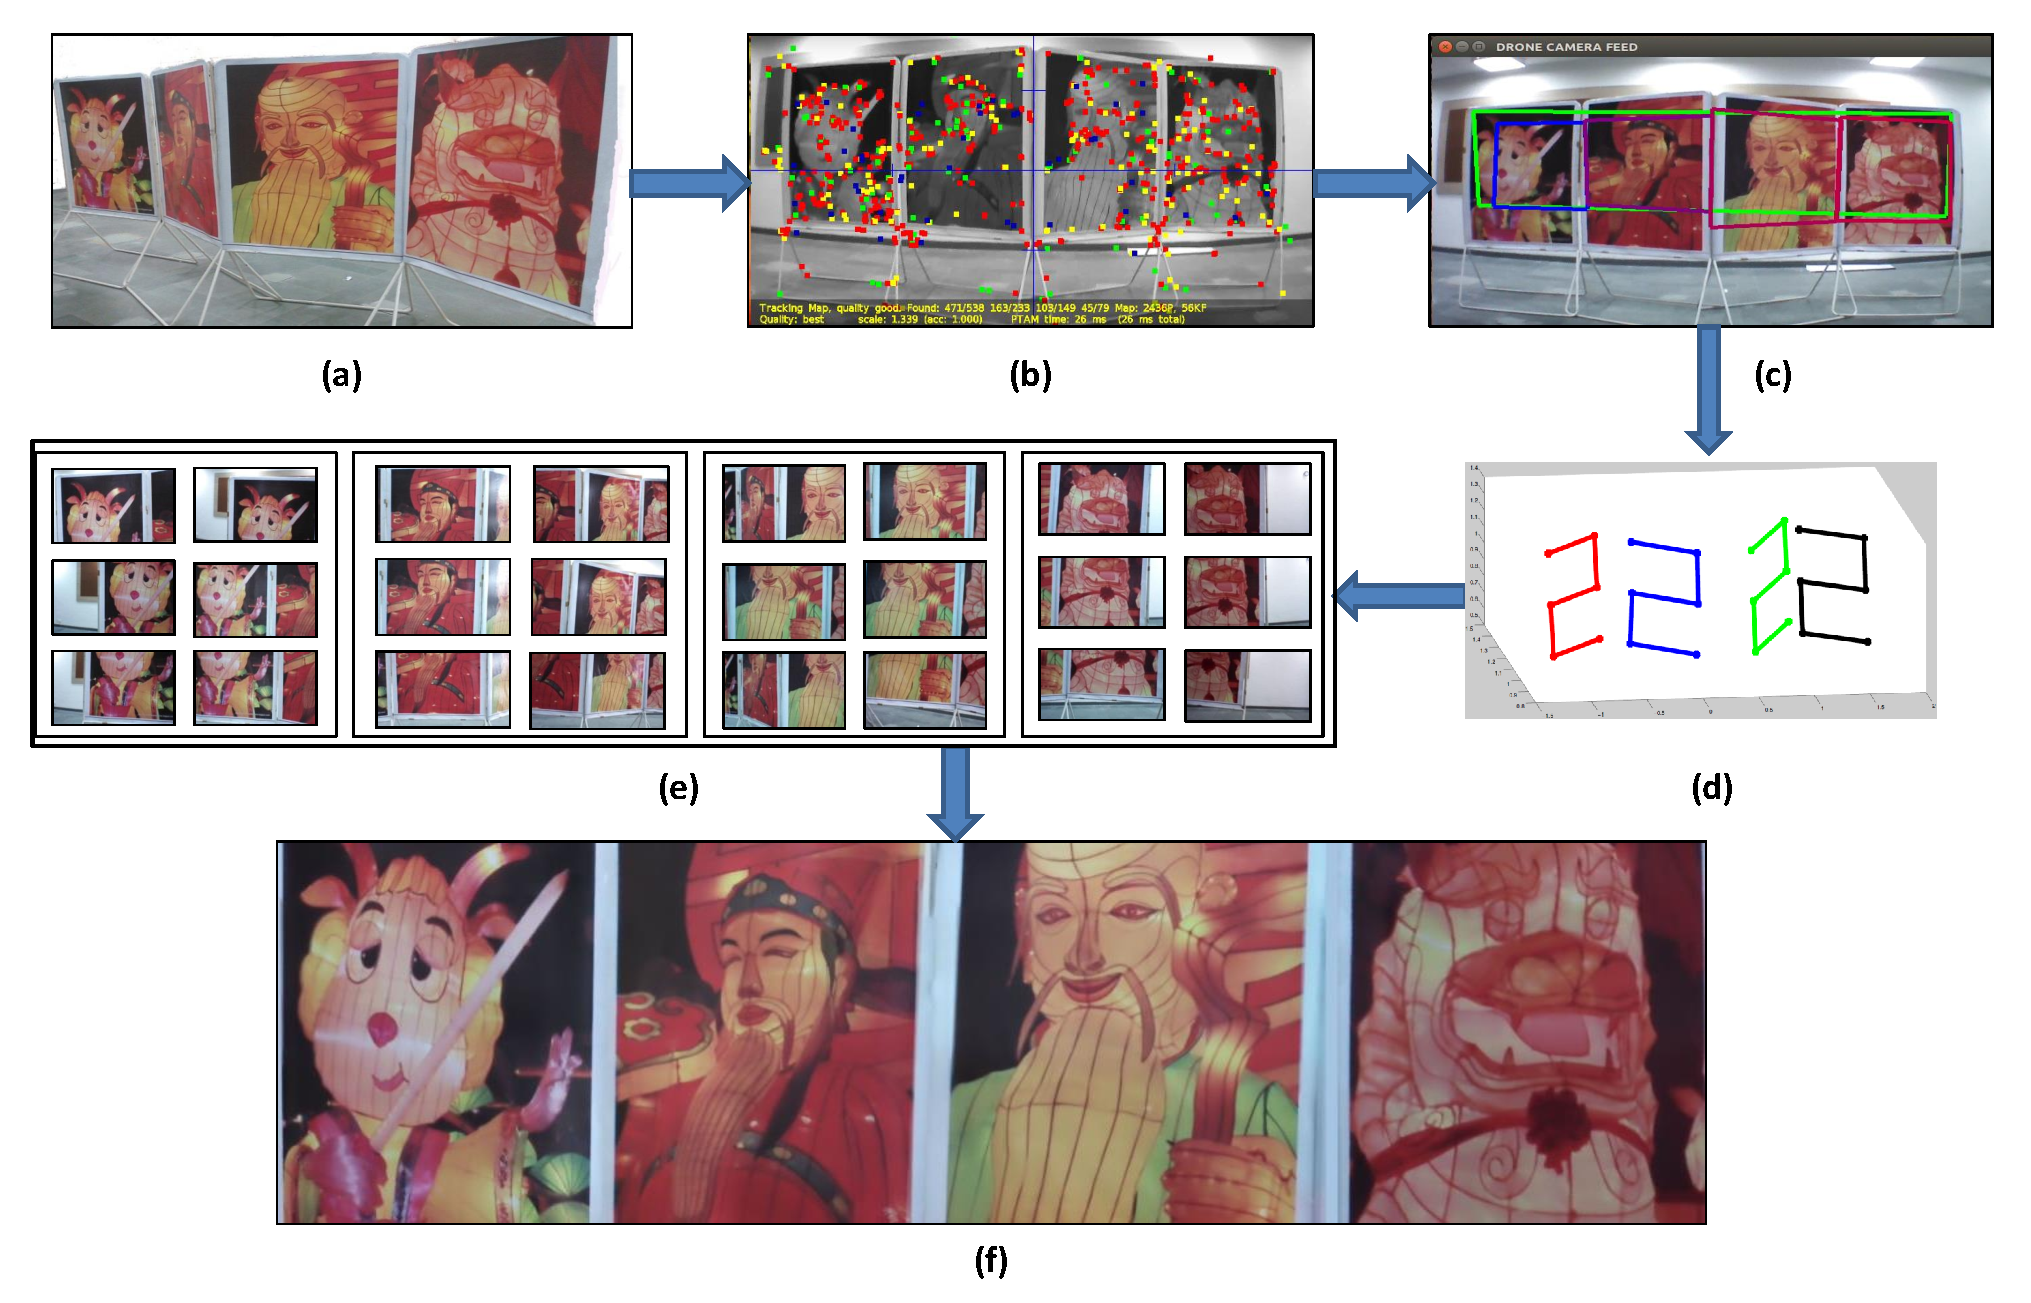
\includegraphics[width=\textwidth]{figures/multiplanar/workflow}
\caption[Overall Workflow]{Overview: (a) Input Scene to be imaged. (b) Feature
points in the scene are found and their 3D positions are estimated using scale aware PTAM \cite{engel}. (c) Multiple planar bounded
regions are estimated using our algorithm. (d) For each bounded planar region, 3D camera positions
are calculated and overall path planning is done. (e) Videos are captured at
each target position. From each captured video, the appropriate frame is
found. (f) Individual mosaics are joined together to get final output.}
\label{fig:workflow}
\end{figure}
\subsection{3D map}
We have used PTAM based method \cite{engel} to localize quadcopter as well as to
create a 3D map of surrounding environment (See Figure \ref{fig:ptam_output}).
In PTAM, initially, the prior pose is estimated using motion model. Then the map
points are projected into the image using prior pose estimate. Next, the camera
pose is updated using some of the feature matches in the image. Final pose
estimate is computed from all the matches found.
 
The initial map built from stereo initialization algorithm has an arbitrary
scale. Hence, there is need of scaling map to metric units. This is done by
assuming that the camera is translated 10 cm between the stereo pair. This
assumption may not be true in the case of inexpensive quadcopter due to its jerky
motions. So, proper scale estimation is necessary.

\textbf{Scale Estimation}
The quadcopter measures distance traveled during translation using PTAM as well as
available metric sensors (ultrasound altimeter) at regular intervals. We get
a pair of samples $\mathbf{x}_i, \mathbf{y}_i \in {\Re}^d$ where $\mathbf{x}_i$ is
scaled translation calculated from PTAM system and $\mathbf{y}_i$ is the distance
measured by the metric sensor at each interval. These pair of samples are related
according to $\mathbf{x}_i \approx \lambda \mathbf{y}_i$. The scale $\lambda$ is
estimated by minimizing the negative log-likelihood\cite{engel}.  

We could get the correct pose by  scaling  PTAM estimated pose. But we
cannot rely only on PTAM for pose estimation as visual feedback may lag due to
problems in wi-fi connectivity. Hence there is need of  alternative
mechanism as a fallback to PTAM. Engel et al. \cite{engel} have used Extended
Kalman Filter to fuse odometry observation model with visual observation model for state prediction i.e.,
estimating the pose (x,y,z and roll-pitch-yaw) of quadcopter at given  instant.

\textbf{State Prediction and Observation:} The state space consists of a total
of ten state variables. 
\begin{ceqn}
\begin{align}
	\mathbf{x}_t &\coloneqq {(x_t, y_t, z_t, \dot{x_t}, \dot{y_t},
	\dot{z_t}, {\Phi}_t, {\Theta}_t, {\Psi}_t, \dot{{\Psi}_t} )}^T  \in
	{\mathbb{R}}^{10},
\end{align}
\end{ceqn}
where $(x_t, y_t, z_t)$ represents the position of the quadcopter in
metric units and $(\dot{x_t}, \dot{y_t}, \dot{z_t})$, the velocity in m/s, both
in world coordinates. The state also contains three angles, i.e., the roll
${\Phi}_t$, pitch ${\Theta}_t$ and yaw ${\Psi}_t$ of the drone in degrees.  An observation
function $h(x_t)$ for each sensor as well as respective observation vector $z_t$
composed from the sensor readings is defined for each observation model.

\textbf{Odometry observation model:} Quadcopter measures its horizontal speed
(i..e., along x and y direction) in its local coordinate system which is
transformed into global coordinate system to get $\dot{x_t}$ and $\dot{y_t}$.
The roll and pitch angles are directly taken from the accelerometers'
observations. Height measurements ($\hat{h_t}$) and yaw measurements
($\hat{{\Psi}_t}$) are differentiated and treated as observations of respective
velocities. The resulting observation function $h_I(\mathbf{x}_t)$ and
measurement vector $\mathbf{z}_{I,t}$ is given by,
\begin{ceqn}

\begin{align}
	h_I(\mathbf{x}_t) &\coloneqq  
	\begin{pmatrix} 
		\dot{x_t}\cos{{\Psi}_t} - \dot{y_t}\sin{{\Psi}_t} \\
		\dot{x_t}\sin{{\Psi}_t} + \dot{y_t}\cos{{\Psi}_t} \\
		\dot{z_t} \\
		{\Phi}_t \\
		{\Theta}_t \\
		\dot{{\Phi}_t}   	
	\end{pmatrix}
	\\
	\mathbf{z}_{I,t} &\coloneqq (\hat{v}_{x,t}, \hat{v}_{y,t}, (\hat{h}_t -
	\hat{h}_{t-1}), \hat{{\Phi}_t}, \hat{{\Theta}_t}, (\hat{{\Psi}_t} - \hat{{\Psi}}_{t-1}  ) )^T
\end{align}
\end{ceqn}
\textbf{Visual Observation Model:} The pose estimate is scaled by the
current estimate for the scaling factor ${\lambda}^{*}$ when PTAM tracks a
video frame successfully. This pose estimate is transformed from the coordinate
system of the front camera to the coordinate system of the quadcopter. Direct
observation of the quadcopter’s pose is given by,
\begin{ceqn}

\begin{align}
	  h_P(\mathbf{x}_t) &\coloneqq  {(x_t, y_t, z_t, {\Phi}_t, {\Theta}_t,
	  {\Psi}_t)}^T \\
	  \mathbf{z}_{I,t} &\coloneqq
	  f(\mathbf{E}_{\mathit{DC}}\mathbf{E}_{\mathit{C},t} )
\end{align}
\end{ceqn}

where $\mathbf{E}_{\mathit{C},t} \in SE(3)$ is the estimated camera pose (scaled
with $\lambda$ ), $\mathbf{E}_{\mathit{DC}} \in SE(3)$ the constant
transformation from the camera to the quadcopter coordinate system, and $f :
SE(3) \rightarrow \mathbb{R}^6$ the transformation from an element of $SE(3)$ to
our roll-pitch-yaw representation.

\textbf{Prediction Model:} Extended Kalman filter is used to fuse all state
variables from both observation models. (Please see \cite{engel} for the
details). Finally prediction model describes how state vector $\mathbf{x}_t$
evolves from one time step to next. The quadcopter’s horizontal acceleration is
approximated $\ddot{x}, \ddot{y}$ based on its current state $\mathbf{x}_t$.
Quadcopter's vertical acceleration   $\ddot{z}$, yaw-rotational 
acceleration $\ddot{{\Psi}_t}$ and the roll/pitch rotational speed
$\dot{{\Psi}_t}, \dot{{\Theta}_t}$ is estimated based on the state
$\mathbf{x}_t$ and  active control command $\mathbf{u}_t$. Finally, using quadcopter's 
estimated pose information, we update the 3D map of the environment.

\noindent\textbf{Scale Accuracy:} 
Though \cite{engel}  gives 3D map of the environment, the scale accuracy is not
ensured. It may lead to inaccurate 3D coordinates of the feature points. To
ensure scale is 100 percent accurate, we moved the quadcopter autonomously in
the vertical direction (up and down) by fixed distance. The reason behind moving in
the vertical direction is that the sonar gives us very accurate height information 
which is used to remove scale ambiguity.

We have conducted a small experiment to demonstrate the efficacy of our method to
achieve 100\% scale accuracy. First, we initialized PTAM after
taking off the quadcopter, moved the quadcopter to location (0, 0, 1) i.e., 1
meter above ground, and finally landed it from the same location. Ideally,
take-off location and land location should be same. However, due to errors in
PTAM initialization as well as noise in IMU measurements, the distance between
two locations will be non-zero. We use this distance as a measure of error. We also tried to imbalance the quadcopter, while it is at location (0, 0, 1), before landing to check its
ability to come back to original position.

Later, we repeated the experiment with one change, instead of using only PTAM
initialization, we have autonomously moved the quadcopter up and down by fixed
distance (1 meter) after PTAM initialization. Our summarized observations
after ten runs in both cases are listed in Table~\ref{tab:ptamInit}.
\begin{table}
\centering
\newcolumntype{C}{ >{\centering\arraybackslash} m{2cm} }
\newcolumntype{D}{ >{\centering\arraybackslash} m{5cm} }
\begin{tabular}{|D|C|C|C|C|}
\hline
Case & Avg. Scale Accuracy & Avg. Scale (in m) & Number of Iterations &
Mean Error $\pm$ std. (in cm)\\
\hline
Only PTAM initialization & 0.524 & 1.2 & NA & 82.6 $\pm$ 10.73 \\
\hline
PTAM initialization with accuracy check & 1.0 & 2.33 & 3--4 & 13.2 $\pm3.6$\\
\hline       
\end{tabular}
\caption[Effect of ensuring scale accuracy on pose estimation]{Effect of
ensuring scale accuracy on pose estimation of quadcopter.
The first row shows that with only PTAM initialization, we do not get the accurate pose.
When we use our method to ensure the 100\% scale accuracy, we are much better in
pose estimation. The scene used for this testing was 2.3 meters away from the
quadcopter. As the estimated scale (2.33m) with our method is very close to the
actual distance of the scene from a quadcopter, generated 3D map will be also very
accurate.}
\label{tab:ptamInit}
\end{table}
Table~\ref{tab:ptamInit} clearly indicates that the pose estimate with only PTAM
initialization is far off (around 85cm) from actual position\footnote{We also
noted that sometimes quadcopter was not able to come anywhere near to (0, 0, 1)
if we imbalance a quadcopter purposefully after PTAM initialization.}.
However, when we ensure scale accuracy the estimated pose is within 15 cms of the
actual location. The estimated scale is also very close to the actual distance of
the plane, if we use our method for ensuring 100\% scale accuracy.

\begin{figure}[t!]
\centering
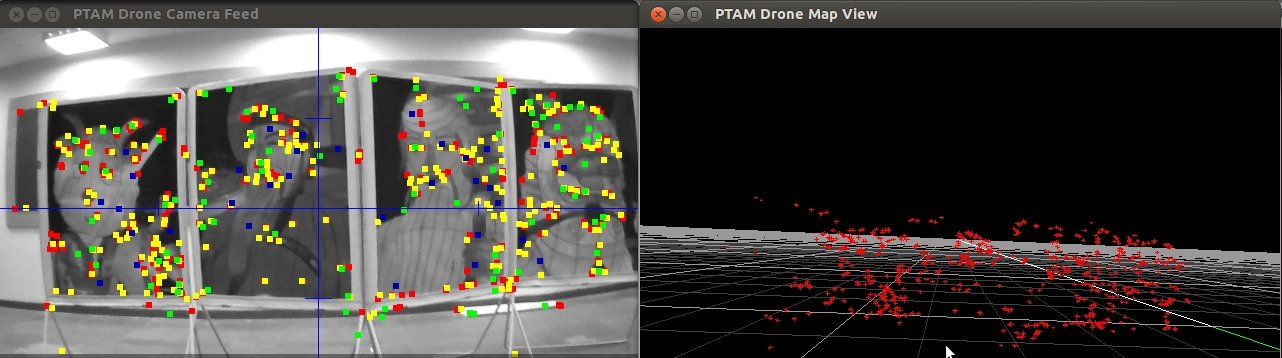
\includegraphics[width=\linewidth]{images/3D_2D}
\caption[Creation of 3D map]{Mapping of 3D locations to 2D image pixel locations
of feature points using PTAM. Left: Camera view showing 2D locations of detected feature points.
Color coding indicates the coarseness level of detected features. Right: Mapview
showing 3D locations of detected feature points.}
\label{fig:ptam_output}
\end{figure}

\subsection{Human Interaction}
Next step after we get a 3D map of the environment is getting the desired area for
imaging from the user. The user may be interested in a scene spread over multiple
planes. Also, the user would like to cover a particular part of it. So we need
to identify the area of interest of the user on the multiplanar surface.
Hence, we  first fly the quadcopter at a sufficiently far distance from the
surface. The distance should be such that the user can see the whole
scene.We have created a user interface which enables the user to mark the region
of interest.\\
\begin{figure}[t!]
\centering
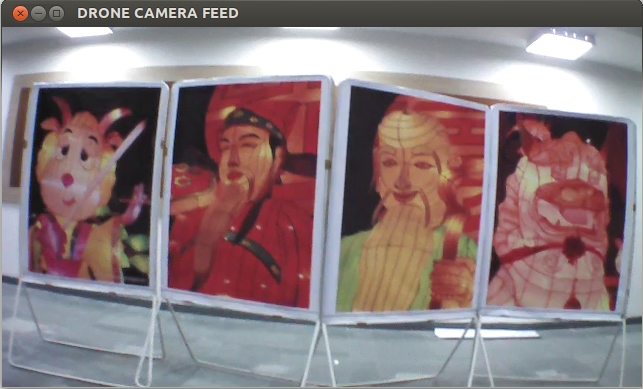
\includegraphics[width=0.31\linewidth]{images/UI_input}
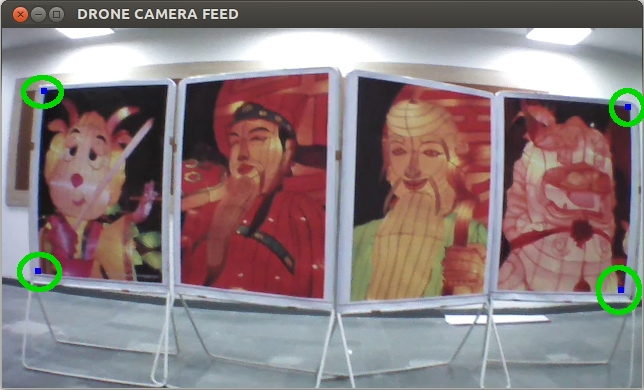
\includegraphics[width=0.31\linewidth]{images/UI_points_marked}
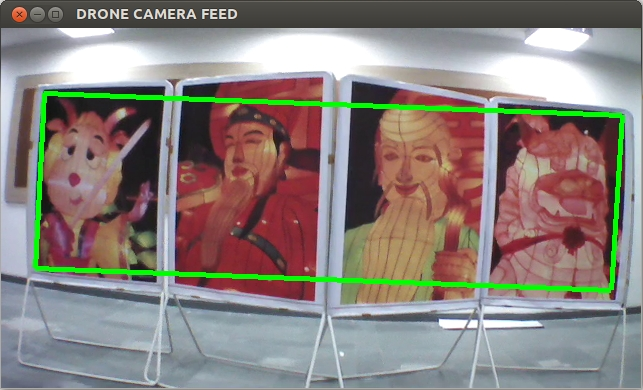
\includegraphics[width=0.31\linewidth]{images/UI_convexHull}
\caption[Our user interface]{Left: The user is shown a live video stream as seen
from a quadcopter camera. Middle: The user may click points to denote the area of interest. We 
find out the nearest 3D point and show its projection (encircled blue pixels) on
the image plane. Right: Once user finishes with clicking points, we find out its convex
hull and show it in green convex polygon.}
\label{fig:ui}
\end{figure}
\textbf{User interface} User is shown the live video stream as seen through
the quadcopter (Figure \ref{fig:ui}(Left)). Now, users can click points to
mark their area of interest on the 2D screen. At backend we determine the
nearest 3D point corresponding to the location clicked by the user and then show
its projection on the image plane. (Figure \ref{fig:ui}(Middle)). Once they
finish with marking the points, they can see the convex hull of the
clicked points in order to check the area to be covered is indeed the area of
interest (Figure \ref{fig:ui}(Right)). The user can optionally add or delete points
or even completely remove all clicked points using the interface.

\subsection{Multiplanar Regions Detection}
We need to detect multiple planes present in the user's region of
interest. There are many algorithms such as Sequential RANSAC\cite{Kanazawa},
multiRANSAC\cite{zuliani} , J-linkage\cite{jlinkage}, T-linkage\cite{tlinkage}
etc. to detect multiple models from the data. But we have chosen real-time
implementation of J-linkage \cite{realtimejlinkage}.\\
\textbf{J-linkage:} Sequential RANSAC and multiRANSAC algorithms require
the number of planes as an input parameter. But as the number of planes changes
according to the input scene, we cannot use these algorithms. J-Linkage and T-Linkage
doesn't require the number of planes as an input parameter. 
%Though T-Linkage is more robust to noise in the input points, it is an order of
%magnitude slower than J-Linkage. 
In our application, detection of the number of planes is the first and most
important step. Hence it needs to be done in real-time which makes J-Linkage
more suitable than T-linkage.

But J-Linkage doesn't give the extent of the plane, i.e., bounded
region. It tries to fit all points to the planes. Figure \ref{fig:multiplane}
depicts the relevant scenario. As we can see, there are some points which may
be the result of inaccurate 3D map generated by PTAM (indicated by a black oval).
As these points have ``geometric'' affinity towards plane A, J-linkage puts these
points in plane A\textquotesingle s cluster. But in the real world, they are part
of plane B.
So we need to disambiguate such points for correct calculation of multiplanar
bounded regions. We have developed an algorithm to modify the output of
J-Linkage to give correct bounded multiplanar regions.\\
\textbf{Improvement over J-Linkage:} JLinkage algorithm output label
for each data point denoting to which plane that data point belongs to. Our
algorithm does following to find continuous multiplanar bounded regions from J-Linkage
output.
\begin{itemize}
  \item Run clustering algorithm e.g., k-means using the output of J-linkage
  as initial labels.
  \item Find out the distance of all points inside each cluster from the cluster
  centroid along the normal of the given plane.
  \item Remove the points from the cluster which are more than 95 percentile
  farther from the cluster centroid along the plane normal.
  \item Find out the bounding rectangle of each cluster.
  \item Extend the rectangle till the intersection with the successive plane.
\end{itemize}

This process is illustrated in Figure \ref{fig:multiplane}. JLinkage
gives us the labeling according to each point's vicinity to the detected
planes. But the 3D points estimated by PTAM may be erroneous due to noise,
marked by circles in Figure \ref{fig:multiplane}(Top). As these points do not
belong to the planes labeled by JLinkage, it gives us wrong bounded
regions. So, we run k-means algorithm using the initial labels given by
JLinkage. Now, points  belong to the correct cluster as shown in
Figure \ref{fig:multiplane}(Middle). But, we don't want points which are far
away from the plane in a normal direction. Hence we remove those points which
are more than 95 percentile farther from the cluster centroid along the plane
normal. We also trim the boundaries of a plane by the bounding box of the
enclosed points. The final output is shown in the Figure
\ref{fig:multiplane}(Bottom).

\begin{figure}[h!]
\centering
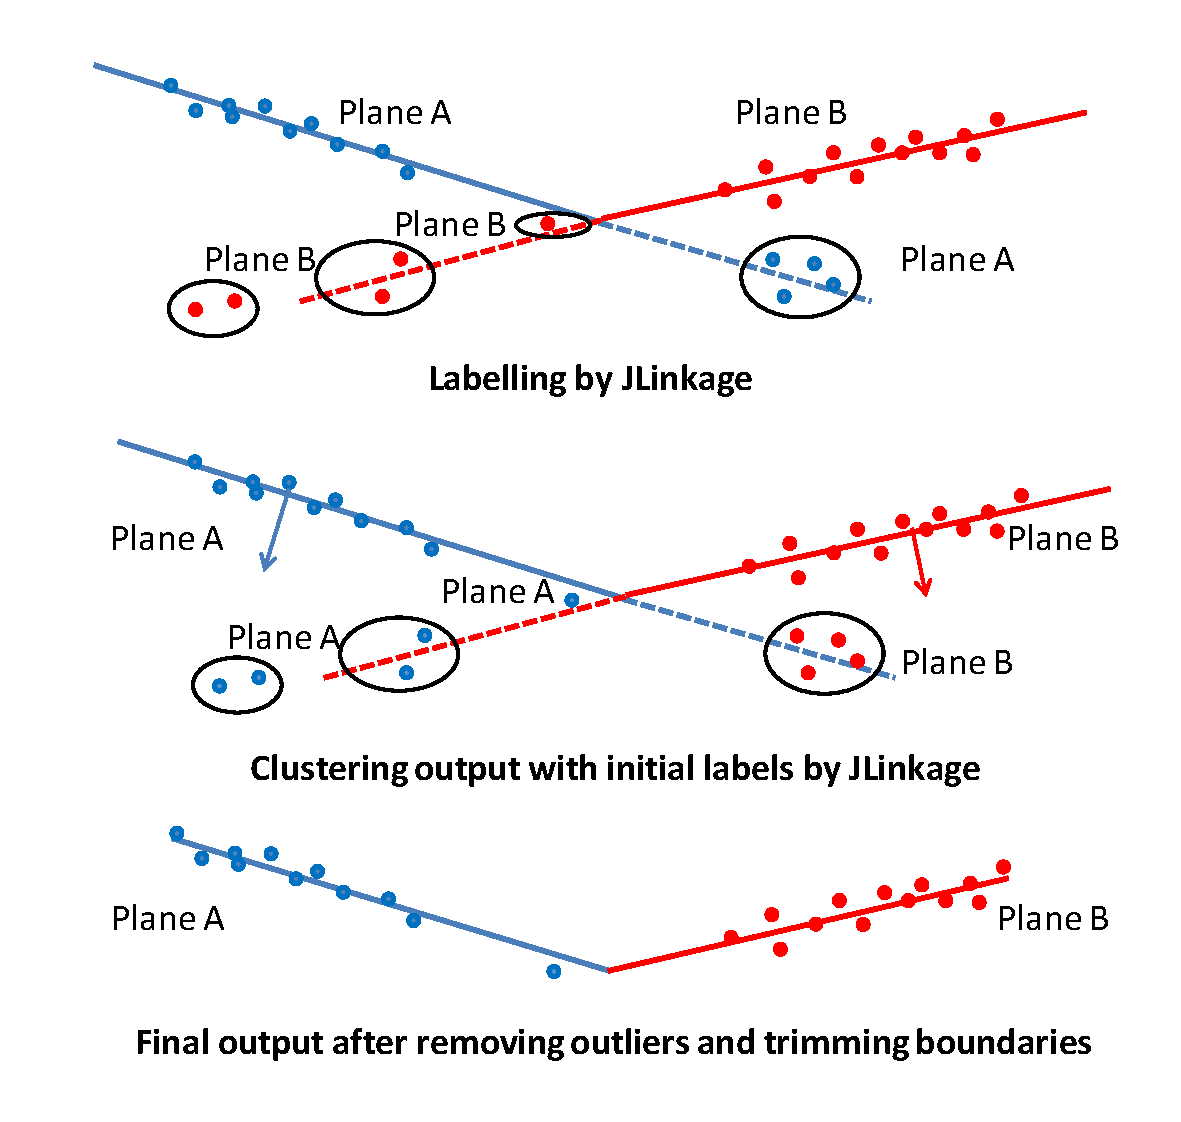
\includegraphics[width=\linewidth]{figures/multiplanar/multiplaneDetection}
\caption[Multiple planes detection]{Process of finding multiplanar bounded
regions from JLinkage output.
The top image shows us the initial labeling given by JLinkage. Later we run a
k-means algorithm using initial labeling given by JLinkage. The output is shown
in the middle figure. Finally, we remove outliers which are farther from the
plane along normal direction and trim boundaries of the plane as shown in
the bottom figure.}
\label{fig:multiplane}
\end{figure}

Each bounded planar region is used to determine the path along which
the quadcopter is navigated to cover that region.

\subsection{Path Planning}
The bounded region is divided into a grid of overlapping cells as shown in
Figure \ref{fig:grid}. We intend to cover each cell in a single image and then
use images from all cells to create a mosaic of given bounded planar
region. Cell area (width, height) is decided on the basis of the amount of details required of the
scene. E.g., if we need to probe our scene with minute details, we have to go
nearer to the plane. So, in that case, cell area is smaller. We need
overlap between neighbor images for successful mosaicing. So, the amount of
overlap between two cells is a function of the required overlap in feature space
needed for stitching. Currently, the overlap is set at thirty percent of cell area to deal
even with sparser (containing fewer feature points) images. Once we
calculate coordinates of cell corners, we determine the desired position of
a camera from where the whole cell area is covered in a single image. We repeat
this process for each cell to find out the path of quadcopter to cover the region in
optimal (in a number of positions) manner so that whole region is covered.

\begin{figure}[h!]
\centering
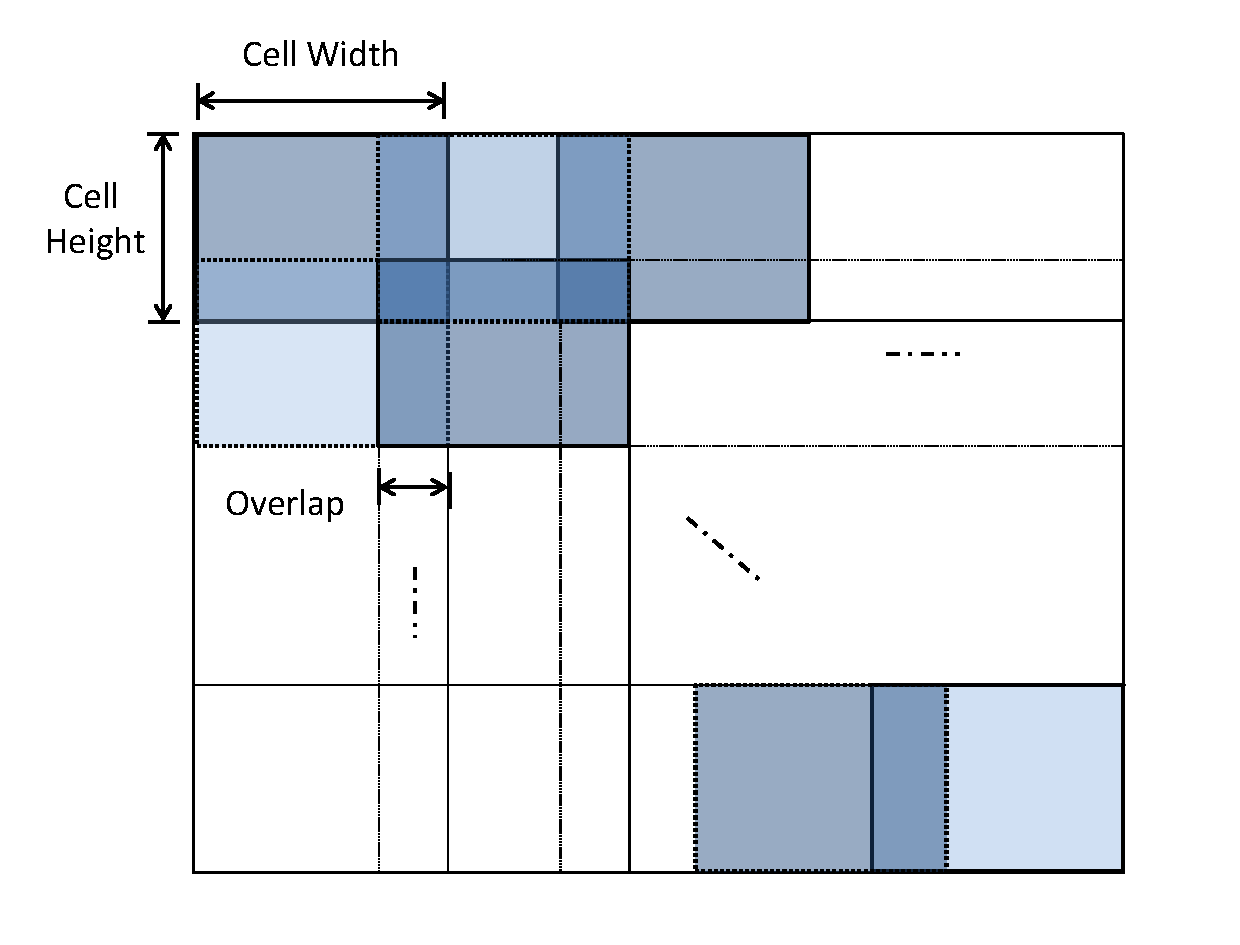
\includegraphics[width=\linewidth]{figures/multiplanar/PathPlanningGrid}
\caption[Path planning]{Grid of overlapping cells designed for path planning.
There is such grid for each planar bounded region. Cell Width and Cell Height is decided based
on the area we would like to capture in one frame. Overlap parameter is
a function of overlap required in feature space for successful stitching.
We find camera position for each cell in the grid which in turn
gives us the path for quadcopter to cover the given planar bounded region.}
\label{fig:grid}
\end{figure}

\subsection{Navigation of a quadcopter}
 We use the pose estimate provided by PTAM  based method \cite{engel}to track
 the quadcopter during navigation along the planned path.\\
\textbf{Covering a single planar bounded region}:
We navigate the quadcopter smoothly in a ``snake scan'' manner along the target points estimated in path
planning step to cover each planar bounded region.\\
\textbf{Transition from one plane to another plane}: We make sure the
transition in terms of yaw as well as horizontal movement is smooth. In order to achieve this,
we divide the horizontal distance into three parts and  move along x and y-axis
alternatively. During each step, we change the yaw in equal proportion so that
the quadcopter’s view is not changed drastically which is very important for
tracking using PTAM \cite{engel}.

\subsection{Recording video and ROS streams}
%AR Drone doesn't have the capability of taking still photographs. 
 We are not sure about the exact position of a quadcopter while capturing
 images due to an error in PTAM as well as the jerky motion of quadcopter. So, we record a video on USB device onboard quadcopter for a small amount
 of time (3 seconds) when we are in proximity of the specified point calculated in path planning. We
also record ROS streams (image as well as navigation data) captured over Wi-Fi.\\
\textbf{Finding the sharp and exact image from video:} We need to find the sharp
image i.e., an image with the minimum blur which is closest to the target point
from 3 seconds HD video (approximately 90 images). But there is no positional data
available on USB device. Navigational data and image streams captured over Wi-Fi help us
in this process. First, we synchronize these two streams using timestamp
information. It gives us an approximate position of each image from the image
stream. Now we select the sharpest image among the images which are taken from
positions in a close proximity of the specified point. Later we match each
image from the HD video with the selected image from the image stream using SURF
features. And finally we select the sharpest image from the HD video among
all images (from the HD video) which are within a threshold in SURF\cite{Bay}
feature space from the selected image from the image stream.

\subsection{Creating mosaic of the multiplanar bounded region}
Once images for each planar bounded region are found from captured
videos, mosaic for each planar region is created using the method of creation of
a mini-panorama presented in \cite{Prasad16}. In \cite{Prasad16}, first images
are arranged in a rectangular grid according to their positions. Here, as we already have grid
information (created in path planning step), our first step is partially done.
Later, we do feature matching among the neighborhood images and create the
maximum spanning tree using  the homography inliers as weight. Finally, mosaic
i.e., mini-panorama is created by warping images according to the respective
homography matrix (w.r.t. the  reference image).

After the creation of mini-panorama for each planar region, we join all
mini-panoramas using a method similar to the creation of super panorama used in
\cite{Prasad16}. In \cite{Prasad16}, the super-panorama is created by finding the
disparity between the reference images of each mini-panorama using the distance
between the camera and the imaging plane and, camera positions of reference
images for each mini-panorama. As all mini-panoramas were in the same plane,
simple stereo formulation (without rectification) was enough. In our case, as
mini-panoramas belong to multiple planes, we need to make sure that all
mini-panoramas are in the same plane to find the disparity among reference images of
 all mini-panoramas, which requires image rectification. But, as we keep the
 quadcopter's camera normal to the plane while capturing reference image for each
 mini-panorama, we don't have to do full rectification.
 We just need to calculate the distance between the center of projections, projected on the imaging plane, 
 along the planes as shown in Figure \ref{fig:multiplanarMosaic}.

\begin{figure}[ht!]
\centering
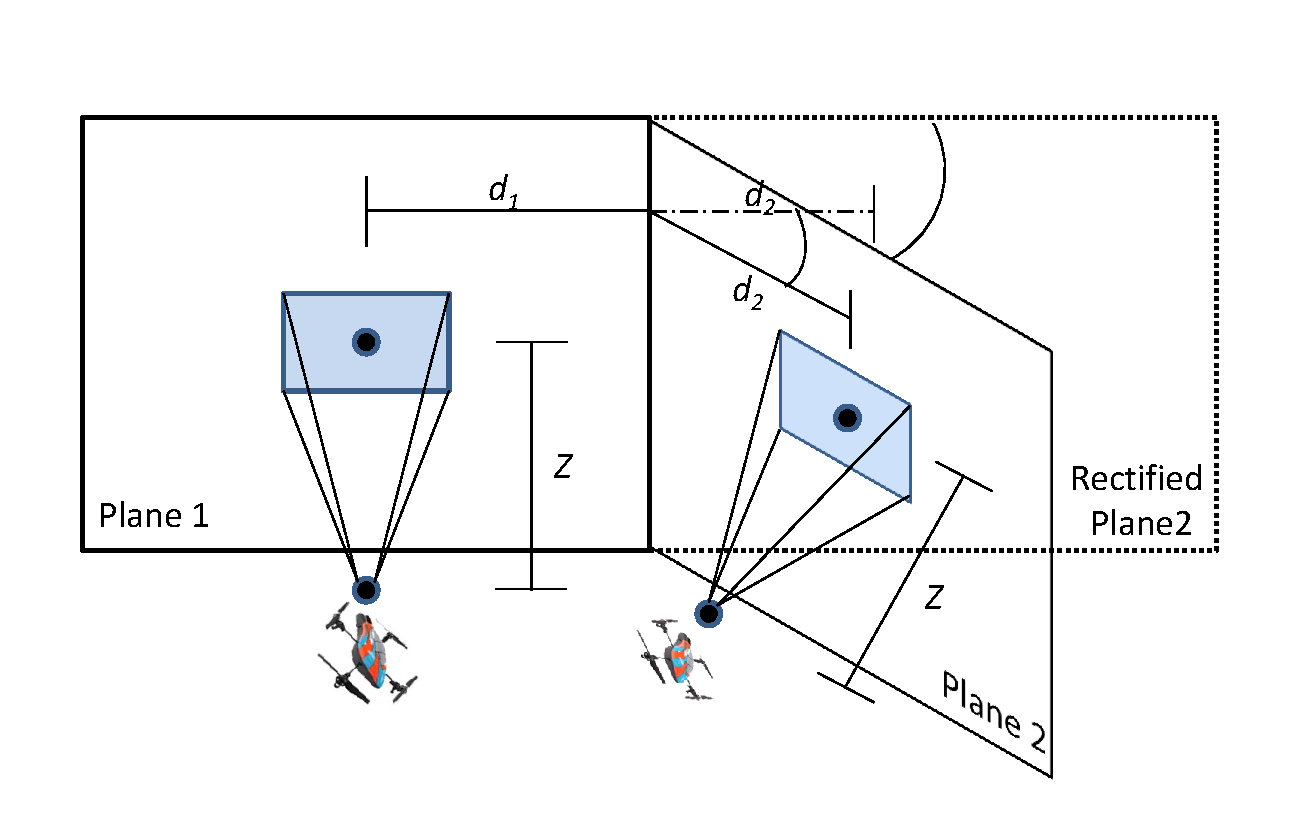
\includegraphics[width=\linewidth]{figures/multiplanar/MultiplanarMosaic}
\caption[Super panorama for multiplanar scene]{Process of finding disparity
between reference images of mosaics imaged on two different planes.}
\label{fig:multiplanarMosaic}
\end{figure}

Let us assume that the depth of the camera from both imaging planes is same
(say $Z$). Now, the disparity of image on the second plane with respect to the
image on the first plane is given as follows\cite{Prasad16}:
\begin{ceqn}
\begin{align}
\textit{disparity} = \textit{focal length}\frac{(d_1+d_2)}{Z}
\label{eq:disparity}
\end{align}
\end{ceqn}

where $d_1$ and $d_2$ are distances of back-projections of the center of
projections on the first and second plane respectively from the line of
the intersection between two planes and $Z$ is the distance between the center of
projection and the plane.

If center of projections are at different depths (e.g., say $Z_1$ and
$Z_2$), first we bring the image at lesser depth (say $Z_1$) to the same depth
of another image (which is imaged at larger depth, say $Z_2$) by zooming out by
fraction $\frac{Z_1}{Z_2}$. Later, we use Eq. \ref{eq:disparity} to calculate
the disparity by setting $Z=Z_2$.

\section{Experiments and Results}
All our experiments have been completed with the inexpensive consumer
quadcopter called  Parrot’s AR Drone 2.0. The camera resolution of AR Drone 2.0
is 1280 $\times$ 720\footnote{But when we stream the image over Wi-Fi the resolution
of an image is 640 $\times$ 360.}. We have used ROS based ARDrone Autonomy
Driver to communicate with the drone. For the purpose of showing the efficacy
of our method, we also took a picture of the scene from a distance with a 5
mega-pixel camera to better understand the scene. We have implemented our
algorithm in C++ using the OpenCV library (OpenCV 2.4.9).  Experiments were
performed on a laptop with Intel Core i5 processor(@2.4GHz) and 8GB RAM.

\subsection{Single Plane with Multiple Visits}
We have first used our algorithm to image a single planar wall shown in
Figure \ref{fig:resultLady}(Left). As the wall was too tall and it was not
possible to see the complete wall in one flash due to a shortage of space, we selected the
desired area in two steps as shown in Figure  \ref{fig:resultLady}(Middle). In path planning 37 (12
for the top and 25 for the bottom) positions were estimated to cover full region. Images
captured from those positions are mosaiced using our algorithm to get final
mosaicing output as shown in Figure \ref{fig:resultLady}(Right).

\begin{figure}
\centering
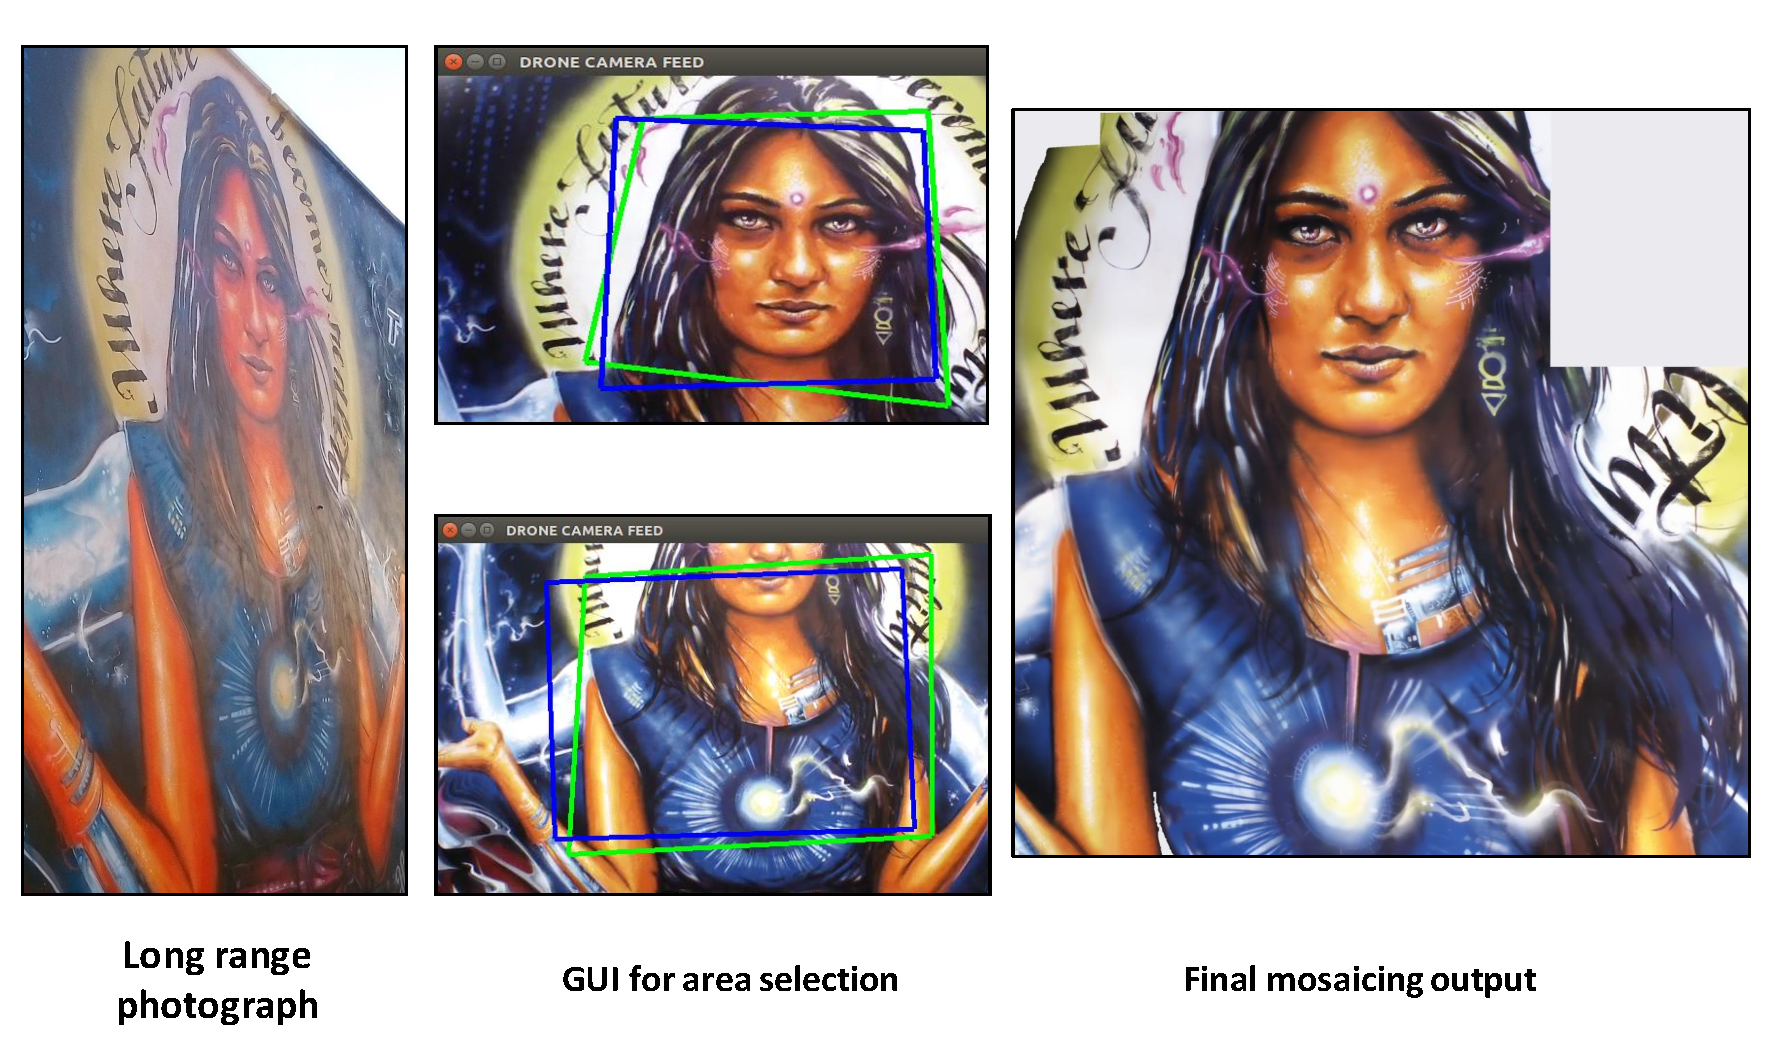
\includegraphics[width=\linewidth]{figures/multiplanar/ladyResult.pdf}
\caption[Result: Single planar scene]{There is a 15 feet tall wall as shown in
the long range photograph (left) which we would like to cover orthographically and with details. We cannot
select the whole area in a single instance as we cannot go back to see the whole
wall. Hence, we selected the desired area in two steps as shown in GUI for area
selection (middle-top and middle-bottom). Green quadrilateral shows user selected area
while blue quadrilateral shows the planar bounded region estimated by our
algorithm. In path planning 37 (12 for the top and 25 for the bottom) positions were
estimated to cover the full region. Images captured from those positions are
mosaiced using our algorithm to get the final mosaicing output as shown in the
right image.}
\label{fig:resultLady}
\end{figure}

\subsection{Multiple Planes}
Our further experiments are done on various setups covering multiple planes.\\

\textbf{Concave:} In this experiment, the exhibits were arranged in the concave
fashion as shown in Figure \ref{fig:resultConcave}(Top-Left). We have selected
the area to be imaged as shown in Figure \ref{fig:resultConcave}(Top-Right). In
the path planning stage, overall 27 (9 from the left plane, 12 from the middle and 6
from the right plane) positions were estimated to cover full region. Images captured
from those positions are mosaiced using our algorithm to get the final mosaicing
output as shown in the Figure \ref{fig:resultConcave}(Bottom).

\begin{figure}
\centering
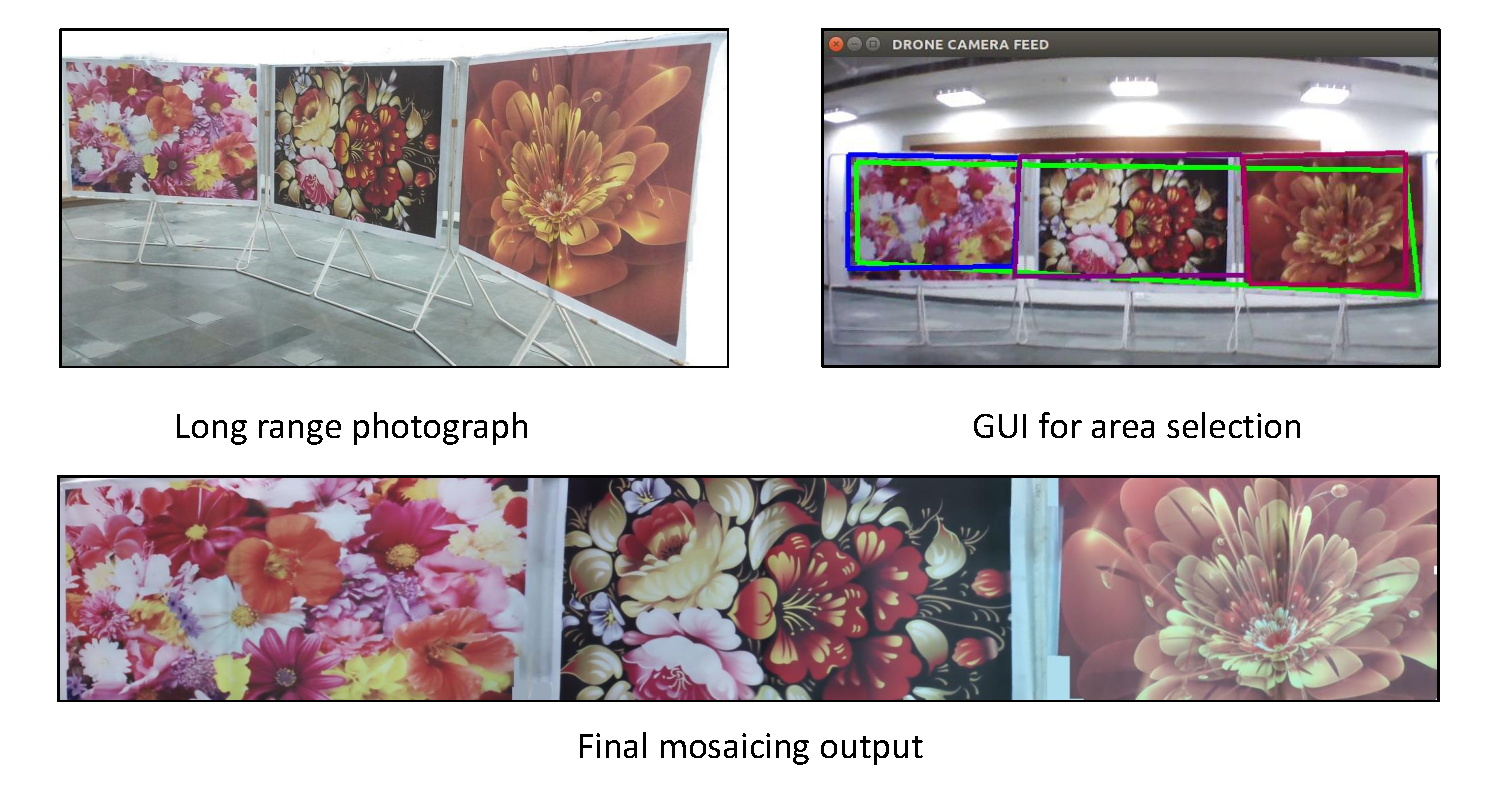
\includegraphics[width=\linewidth]{figures/multiplanar/ConcaveResult.pdf}
\caption[Result: Concave arrangement]{There is an art exhibition containing
multiple posters arranged in concave fashion as shown in the long range photograph (top-left). We have
selected the area to be imaged as shown in GUI for area selection(top-right).
Green quadrilateral shows user selected area while blue, violet and magenta
colored quadrilaterals represent the multiple planar bounded regions
estimated by our algorithm. In the path planning stage, overall 27 (9 from the left
plane, 12 from the middle and 6 from the right plane) positions were estimated to cover
full region. Images captured from those positions are mosaiced using our algorithm
to get the final mosaicing output as shown in the bottom image.}
\label{fig:resultConcave}.
\end{figure}

\textbf{Convex:} In this experiment, paintings were arranged in the convex
fashion as shown in Figure \ref{fig:resultConvex}(Top-Left). We have selected
the area to be imaged as shown in Figure \ref{fig:resultConvex}(Top-Right). In
the path planning stage, overall 30 (9 from the left plane, 12 from the middle and 9
from the right plane) positions to cover full region are estimated.  Images
captured from those positions are mosaiced using our algorithm to get the final
mosaicing output as shown in the Figure \ref{fig:resultConvex}(Bottom).

\begin{figure}[t!]
\centering
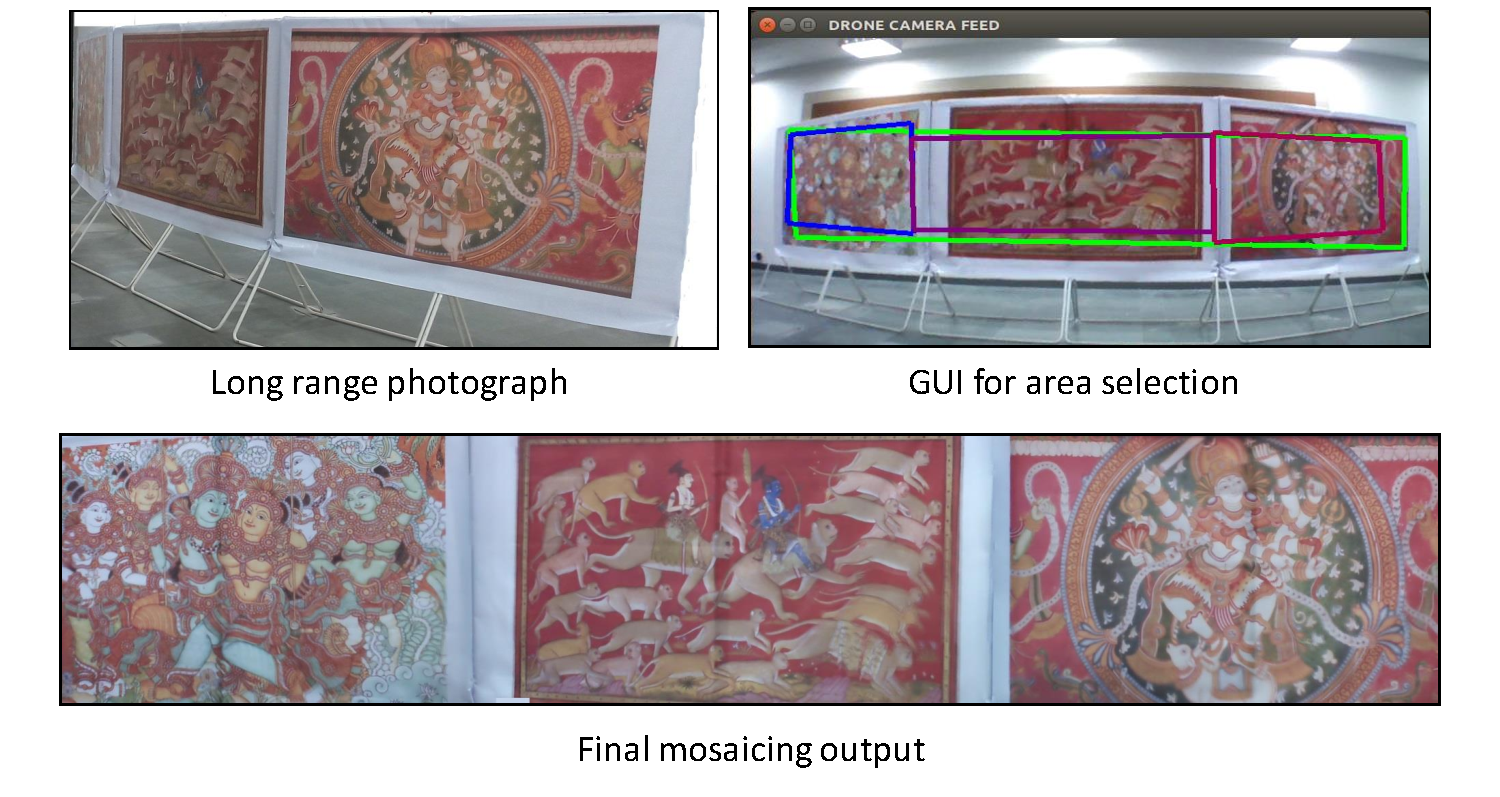
\includegraphics[width=\linewidth]{figures/multiplanar/convexResult.pdf}
\caption[Result: Convex arrangement]{There is an exhibition of Indian temple
paintings arranged in convex fashion as shown in the long range photograph (top-left). Note that we
cannot cover all paintings with enough details simultaneously. We have selected
the area to be imaged as shown in GUI for area selection (top-right).
Green quadrilateral shows user selected area while blue, violet and magenta
colored quadrilaterals represent the multiple planar bounded regions
estimated by our algorithm. In the path planning stage, overall 30 (9 from the left
plane, 12 from the middle and 9 from the right plane) positions were estimated to cover
the full region. Images captured from estimated positions are mosaiced using our
algorithm to get the final mosaicing output as shown in the bottom image.}
\label{fig:resultConvex}
\end{figure}

\textbf{Mixed:} We have performed a couple of experiments where posters were
arranged in mixed fashion. First arrangement looked like Figure
\ref{fig:resultMixed1}(Top-Left) where middle posters form convex region while
side posters form concave region. The selected area for imaging is shown in
Figure \ref{fig:resultMixed1}(Top-Right). In path planning overall 24 (6 from each
plane) positions are estimated to cover full region. Images captured from
those positions are mosaiced using our algorithm to get the final mosaicing
output as shown in the \ref{fig:resultMixed1}(Bottom).

\begin{figure}[t!]
\centering
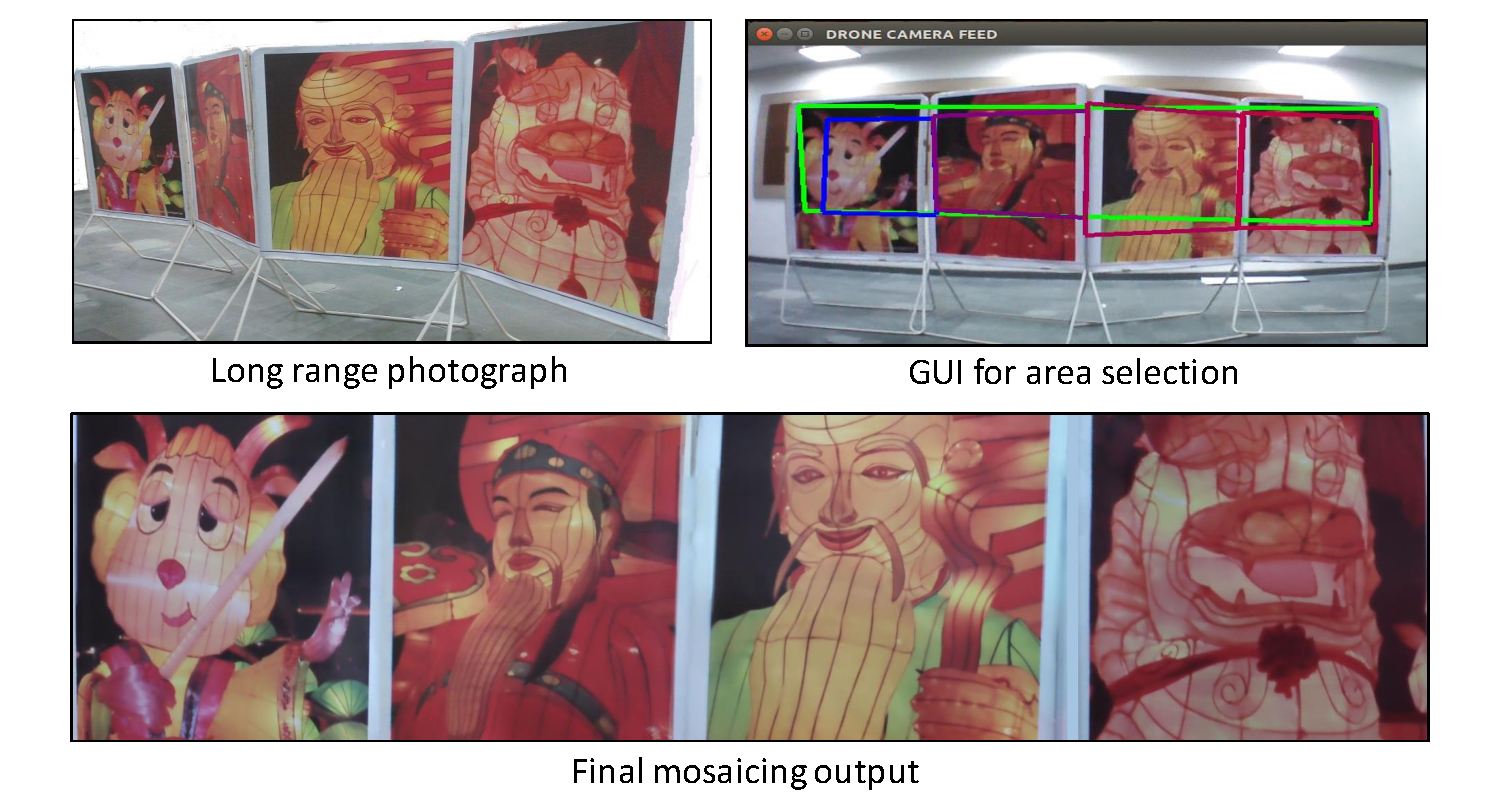
\includegraphics[width=\linewidth]{figures/multiplanar/mixed1Result.pdf}
\caption[Result: Mixed arrangement]{There is an exhibition of Chinese lanterns'
posters arranged in mixed (concave and convex) fashion as shown in the long range photograph
(top-left). Note that we cannot cover all paintings with enough details
simultaneously. We have selected the area to be imaged as shown in GUI for
area selection (top-right). Green quadrilateral shows user selected area while
blue, violet and magenta colored quadrilaterals represent the multiple
planar bounded regions estimated by our algorithm. In the path planning overall
24 (6 from each plane) positions were estimated to cover the full region. Images
captured from estimated positions are mosaiced using our algorithm to get the
final mosaicing output as shown in the bottom image.}
\label{fig:resultMixed1}
\end{figure}

In the second mixed arrangement, middle posters form concave region while
 side posters form convex region as shown in Figure
\ref{fig:resultMixed2}(Top-Left). The selected area for imaging is shown in
Figure \ref{fig:resultMixed2}(Top-Right).  In path planning overall 24 (6 from
each plane) positions were estimated to cover full region. Images captured from
estimated positions are mosaiced using our algorithm to get the final mosaicing
output as shown in the Figure \ref{fig:resultMixed2}(Bottom).

\begin{figure}
\centering
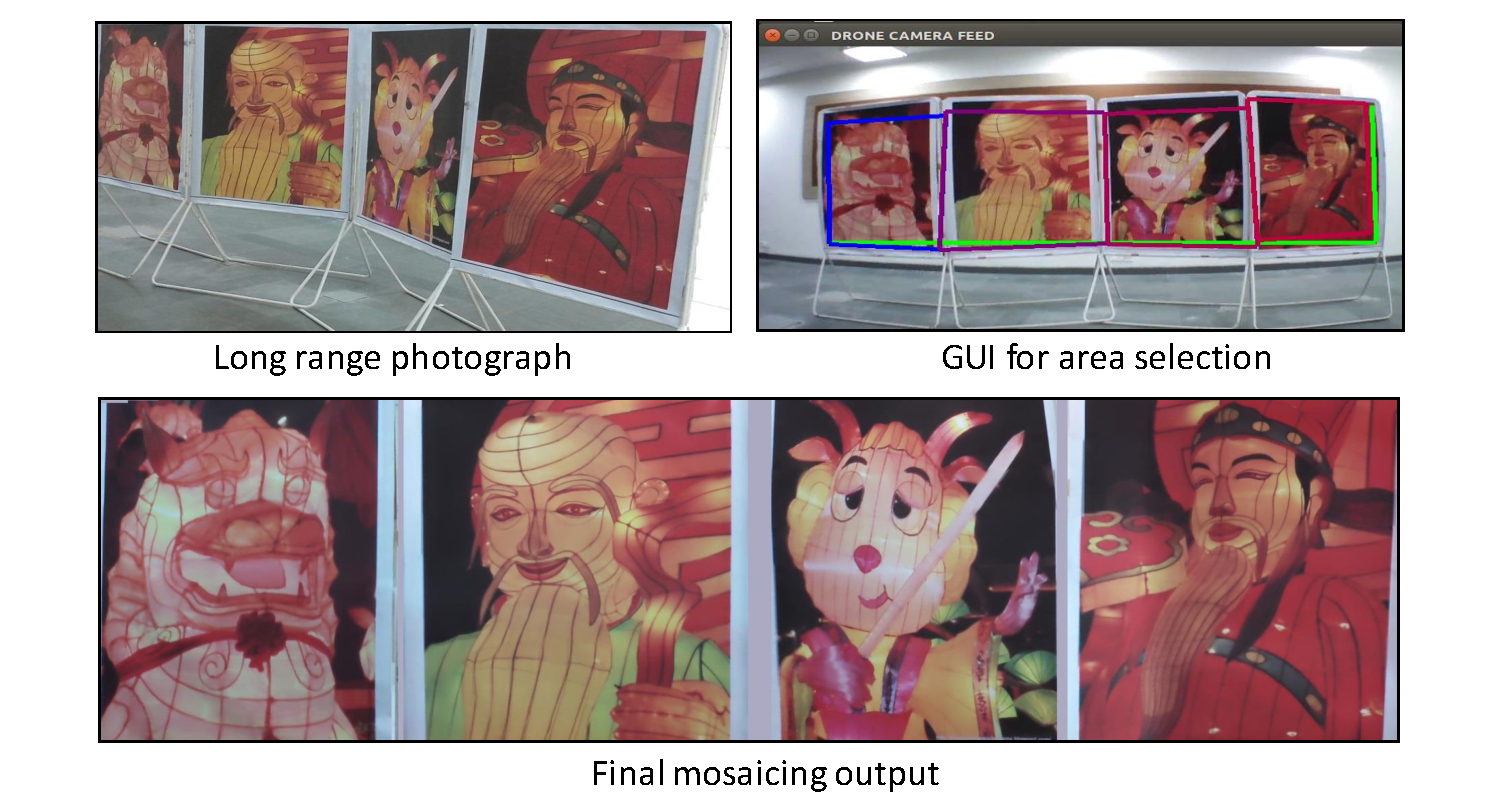
\includegraphics[width=\linewidth]{figures/multiplanar/mixed2Result.pdf}
\caption[Result: Mixed arrangement]{There is an exhibition of Chinese lanterns'
posters arranged in mixed (concave and convex) fashion as shown in the long range photograph
(top-left). Note that we cannot cover all paintings with enough details
simultaneously. We have selected the area to be imaged as shown in GUI for
area selection (top-right). Green quadrilateral shows user selected area while
blue, violet and magenta colored quadrilaterals represent the multiple
planar bounded regions estimated by our algorithm. In the path planning
stage, overall 24 (6 from each plane) positions were estimated to cover the full
region. Images captured from estimated positions are mosaiced using our
algorithm to get the final mosaicing output as shown in the bottom image.}
\label{fig:resultMixed2}
\end{figure}

\textbf{Planes at different depth:} In this experiment we have arranged posters
parallel to each other, but at different depths, as shown in Figure
\ref{fig:resultFrontBack}(Top-Left). It is not possible to mosaic them together
due to change in planes. But we have imaged each exhibit independently using
quadcopter and brought the mosaic of an exhibit at a larger depth to the same depth
of lesser depth exhibit mosaic using the estimated plane equations' information.
The final result is shown in the Figure \ref{fig:resultFrontBack}(Bottom).
\begin{figure}
\centering
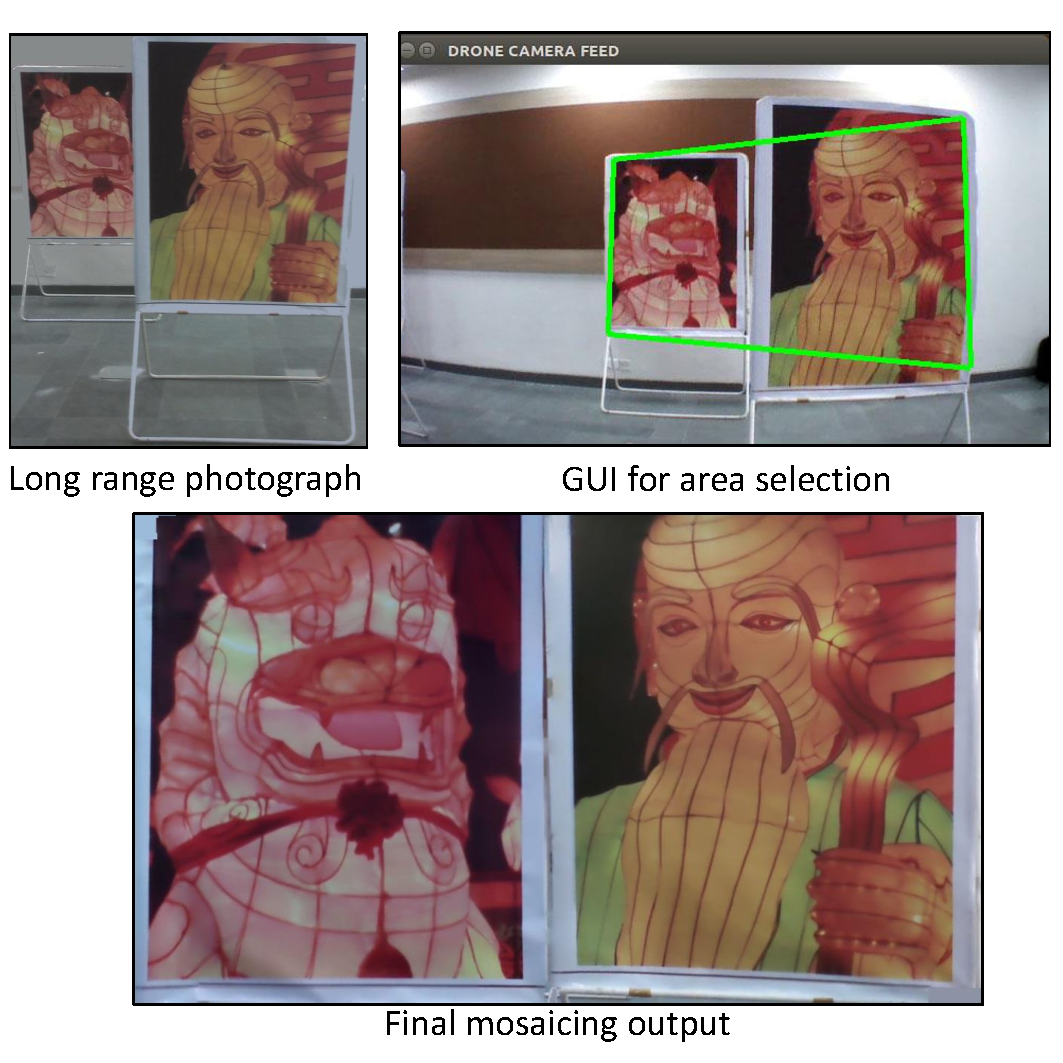
\includegraphics[width=\linewidth]{figures/multiplanar/frontback.pdf}
\caption[Result: Imaging at different depths]{There are two Chinese lanterns'
exhibits arranged parallel to each other but having different depths as shown in the long range
photograph(top-left). It is not able to mosaic both of them in a single
panorama due to the difference in depths. But we imaged those exhibits
independently through a quadcopter and brought the mosaic of an exhibit at larger
depth to the same depth of lesser depth exhibit mosaic. The final result is
shown in the bottom image.}
\label{fig:resultFrontBack}
\end{figure}

\section{Concluding remarks}
We have developed an end-to-end application for autonomously imaging multiplanar
regions using a quadcopter. We have also developed an algorithm for `unrolling'
the multiplanar scene using the fusion of IMU data and video captured from
quadcopter. Homography-based stitching cannot be used to create the mosaic of
scene spread over multiple planes. Also, using the handheld camera is cumbersome
to cover large multiplanar surfaces. Even with the UAVs manual control is very difficult.

In our solution, we autonomously maneuver quadcopter along the planned path to
cover each plane in a multiplanar surface. The path planning for each plane is
done to estimate optimal locations such that images from estimated locations will cover
the whole plane. Later, we stitch images for each plane to create mini-panorama.
Finally, mini-panoramas are merged using positional information to form a full panorama.
Our method works in various setups like convex, concave as well as mixed.

%In the future, our method may be extended to cover any parametric surface in
%general.
It is practically impossible to image very large multiplanar surface using
just single quadcopter due to battery constraint. We can use multiple
quadcopters in collaboration to overcome this limitation. However, we need to
identify each quadcopter accurately to send proper commands. Identification of
a moving object in the unknown environment is a challenging task. Generally, 
fiducial markers are placed on an object for tracking. Motion blur introduced
due to swift movements of quadcopter causes problem in detection of current
fiducials. We discuss the design of motion blur resilient fiducials as well as
the detection of the same in next chapter.

\chapter[Blur Resilient Fiducials]{A Motion Blur Resilient Fiducial For
Quadcopter Imaging}
\label{ch:fiducial}

The recent availability of low-cost quadcopters such as ARDrone 2.0 has helped 
fuel significant efforts in research focused on unmanned aerial
vehicles. Navigation and planning
of these vehicles is typically~\cite{Davison:2007,Engel12,Engel13}
performed using onboard inertial sensors and/or vision based modules
that uses visual cues in the real world. However, to evaluate the
effectiveness of navigation methods, one or more fiducials are commonly
placed~\cite{Bosnak:2012,Lim09,Klopschitz:2007}
 in the environment to provide additional information that
serves for ground-truth positional measurements.
In order to be effective, fiducial markers (or simply, fiducials) need
to be easily detected in the scene. A variety of fiducials have
been proposed~\cite{NaimarkF02,ARToolkit02,Fiala05,Pitag13,runetag11}
in the literature.  These take the form of binary codes arranged into
rectangular grids~\cite{ARToolkit02,Fiala05} or other geometric
primitives arranged in predefined spatial
patterns~\cite{NaimarkF02,Pitag13,runetag11}.  Figure \ref{fig:fiducial_teaser}
shows the popular ARTag \cite{Fiala05} fiducial as possibly seen from
a quadcopter.

\section{Challenges}
\label{sec:intro}
 A problem for existing fiducials is that low-cost
quadcopters often exhibit very quick and erratic physical movements
that result in motion blur evidenced in the images captured from the quadcopter's onboard
camera. This motion blur has an adverse effect on the recognition of fiducial
markers. This can be seen in Figure \ref{fig:fiducial_teaser}--(b) where the
ARTag fiducial cannot be recognized due to motion blur. This is not
too surprising as most existing fiducials are not designed to handle
motion blur.

Compounding this problem is the additional issue of dropped video
frames from the quadcopter's wireless communication module. This means
that not only is blur a problem, but there may be large
discontinuities in the pattern's position due to missing video
frames. This problem makes it challenging to apply tracking algorithms that can
exploit temporal coherence for determining the fiducial's position.

\noindent\textbf{Contributions:}~~To address these problems, we propose a
fiducial that is designed to be resistant to motion blur. Our design
is based on circles as shown in Figure~\ref{fig:fiducial_teaser}--(c,d). The
design is based on the observation that motion blur from a quadcopter
tends to be linear in nature. As such, when our fiducial is blurred,
there is no blur in the direction perpendicular to the direction of
motion.  This allows the signature of the fiducial to remain intact in
any direction.

When multiple fiducials are present, using concentric rings, we can
treat the presence or absence of a ring as a bit, allowing us to
assign a code to the marker. Our experiments show that these designs can
significantly outperform existing codes in the presence of motion
blur. As far as we are aware, this is the first work to propose a blur
resistant marker, especially in quadcopter settings.

%The remainder of this chapter is organized as follows.  Section~2 gives
%an overview of related work in fiducials, as well as the related
%problem of tracking. Section~2 motivates our fiducial design by
%analyzing the performance of existing codes under motion blur, and
%describes our detection algorithm. Section~3 shows several
%experiments using quadcopter imagery. This is followed by a discussion
%and a summary in Section~4 and Section~5 respectively.

\begin{figure}[t!]
  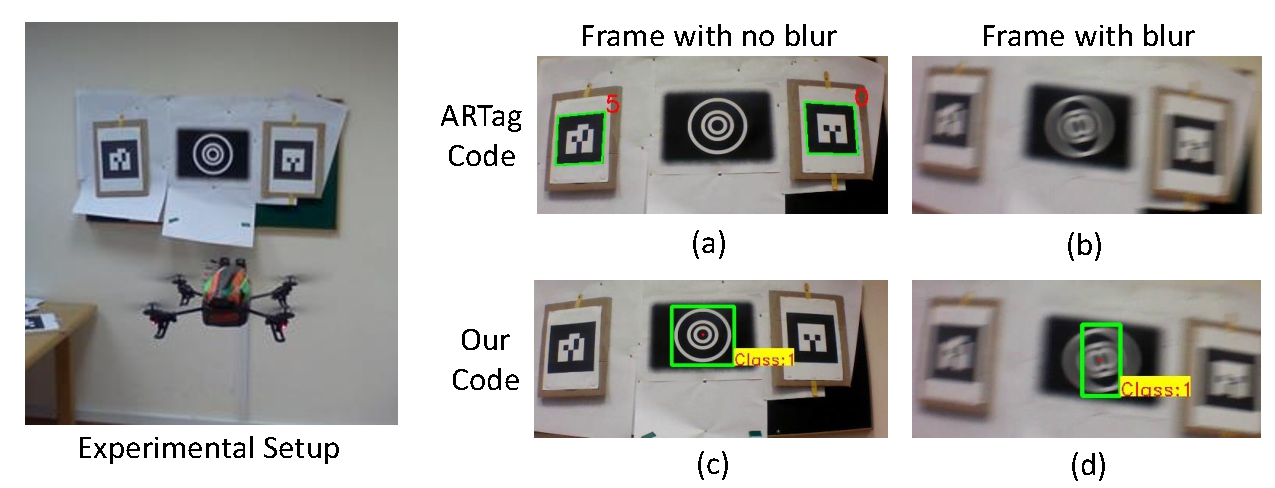
\includegraphics[width=\linewidth]{figures/fiducial/teaser}
  \caption[Overview]{Experimental setup and comparison of fiducial-based
    algorithms. A green border signifies success. 
    \textbf{(Left)} A drone encounters three different fiducials. 
    \textbf{(Right, Top)} Output of ALVAR~\cite{alvar} under favorable and blurred
    circumstances. No green border is seen in (b) signifying failure.
    \textbf{(Right, Bottom)} Output of the proposed fiducial. Green
    border is seen in both (c) and (d).
    \label{fig:fiducial_teaser}}
  \end{figure}

\section{Design of Blur Resistant Fiducial}

We begin by first motivating the need for a new blur resistant
fiducial by examining the performance of prior fiducials under motion
blur.  After this, we detail our design as well as the detection
algorithm used to find the fiducial in an image, or a video sequence.

\subsection{Prior Fiducials Under Motion Blur}\label{sec:blurtest}

Here we examine the performance of two popular fiducials under
motion blur.  Specifically, we examine ARTags ~\cite{Fiala05} and
PiTags~\cite{Pitag13} given their differences in geometric design and
the availability of an API to develop applications to recognize the tags.
\footnote{RUNE-tag~\cite{runetag11} currently does not
provide access to an implementation to generate or recognize its tags. 
The circular data matrix~\cite{NaimarkF02} is available as a
commercial product, however it requires proprietary hardware.}

%To evaluate the ARTag and PiTag under blur, 
For controlled study, we simulate the appearance of the ARTag and PiTag
markers by scaling the tags to 150$\times$150 pixels.
Both fiducials are then blurred using linear motion blur at various
orientations with different  blur scales. The blur motion ranged from 15 to 50
in magnitude (measured in pixels), representing small to significant motion
blur. Figure~\ref{fig:artag_pitag} shows the visual appearance of the blurred
tags. We then try to detect the markers using the ALVAR library~\cite{alvar} and
PiTag library~\cite{ros_pitag}. The table in %the right side of
Figure~\ref{fig:artag_pitag} shows the recognition rate (in
percentage) of the two fiducials at various blur scales over all  orientations.
As we can see, the PiTag performance quickly diminishes under small amounts of
blur, while at 35 units, the ARTag's recognition rate drops to less than
20\%.

\begin{figure}[t!]
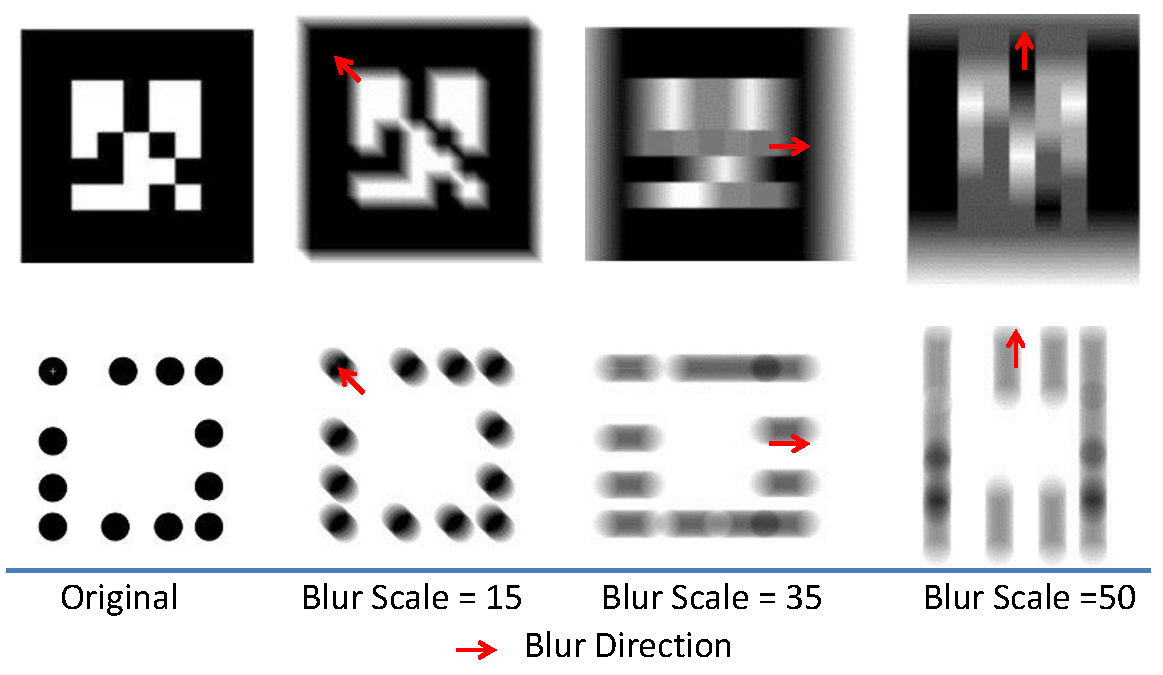
\includegraphics[width=\linewidth]{figures/fiducial/artag_pitag.pdf}
%\captionof{figure}{Blurred ARTag and Pi--tag with various blur scales}
%\captionof{table}{Recognition rate of ARTag and Pi-tag fiducial at various blur scales}

\begin{tabularx}{\linewidth}{|Y|Y|Y|}
\cline{1-3}
\small{Blur} & \multicolumn{2}{c|}{ \small{Recognition Rate}}
\\\cline{2-3}
\small{Scale}& \small{PiTag} &	\small{ARTag} \\ \cline{1-3}
\small{15} & \small{100} & \small{100} \\ %\cline{1-3}
\small{30} & \small{0} & \small{100} \\  %\cline{1-3}
\small{35} & \small{0} & \small{19} \\ %\cline{1-3}
\small{50} & \small{0} & \small{0} \\ \cline{1-3}
\end{tabularx}
\captionof{figure}[Comparison with PiTag and ARTag]{\textbf{Top:} The PiTag and
ARTag fiducials blurred with various blur scales at different orientations. \textbf{Bottom
    Table:} Recognition rate (in percent). We see that the recognition
  rates for both the tags are significantly reduced. For severe blur,
  detection fails.}
\label{fig:artag_pitag}
\end{figure}

\subsection{Blur Resistant Fiducial}

We propose a binary coded fiducial that uses concentric white rings of
equal widths on a black background with a blurred
border\footnote{Obviously, this design can be inverted to have a white
  background with black rings.}. The outermost and innermost rings
represent the start and end of the code and are embedded in the
fiducial.  The binary code is represented by the presence (or absence)
of rings between ``marker'' rings.

\begin{figure}
\centering
  
\includegraphics[width=.24\linewidth]{figures/fiducial/newconcentric_00.pdf}
  
\includegraphics[width=.24\linewidth]{figures/fiducial/newconcentric_01.pdf}
  
\includegraphics[width=.24\linewidth]{figures/fiducial/newconcentric_10.pdf}
  
\includegraphics[width=.24\linewidth]{figures/fiducial/newconcentric_11.pdf}
  \caption[Two-bit binary  fiducials]{Two bit binary  fiducials representing,
  from left to right 00, 01, 10, and 11.}
  \label{fig:fiducials}
\end{figure}

Depending on which ring is present or absent, the resulting binary
code will change. The number of different patterns depends on the
number of bits in the binary code. For example, if the binary code has
three bits, there will be a maximum of three rings between marker
rings and we end up with eight different patterns.
Figure~\ref{fig:fiducials} shows two-bit binary fiducials.


Our fiducial detection strategy is different from
\cite{NaimarkF02,Pitag13} and works under significant amounts of blur.
As previously mentioned, our approach works under the observation that
the motion blur for the quadcopter's camera can be well modeled as
linear motion.  This linear motion blur assumption has been shown to
be reasonable in prior works~\cite{Moshe:2003,Moshe:2004}
targeting camera motion blur. Under this assumption, the scene
content perpendicular to the blur direction is unaffected by the blur.
Because of our circular design, the direction perpendicular to the
linear motion will still be recognizable as a linear pattern.
Figure~\ref{fig:blur_direction} shows examples of this using a pattern
under 
various motion directions.

\begin{figure}[h!]
\centering
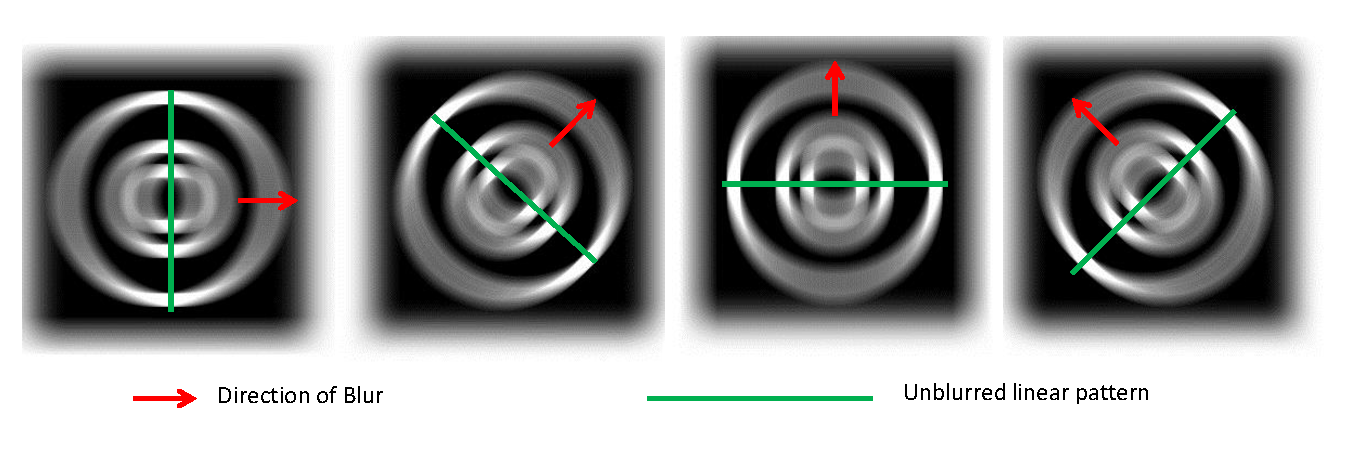
\includegraphics[width=\linewidth]{figures/fiducial/blur_direction}
\caption{Change in blur direction changes the location and orientation
  of an unblurred linear pattern.}
\label{fig:blur_direction}
\end{figure}


\subsection{Detection Algorithm}

Figure~\ref{fig:overall_flow} shows the process involved in fiducial
detection. We give a brief overview of our algorithm here with each
step described in detail afterward.  Our detection algorithm has four
steps. In Step~1, we apply a Gabor filter on the image to isolate the
potential locations of the pattern.  In Step~2, we find clusters of
patches in the Gabor output.  In Step~3, we perform Principal
Component Analysis (PCA) on each cluster to find the dominant
direction unaffected by blur.  Finally in Step~4, based on the
direction detected, we extract the intensity profile of the pattern
and classify the fiducial. 

\begin{figure*}[ht!]
  \centering
  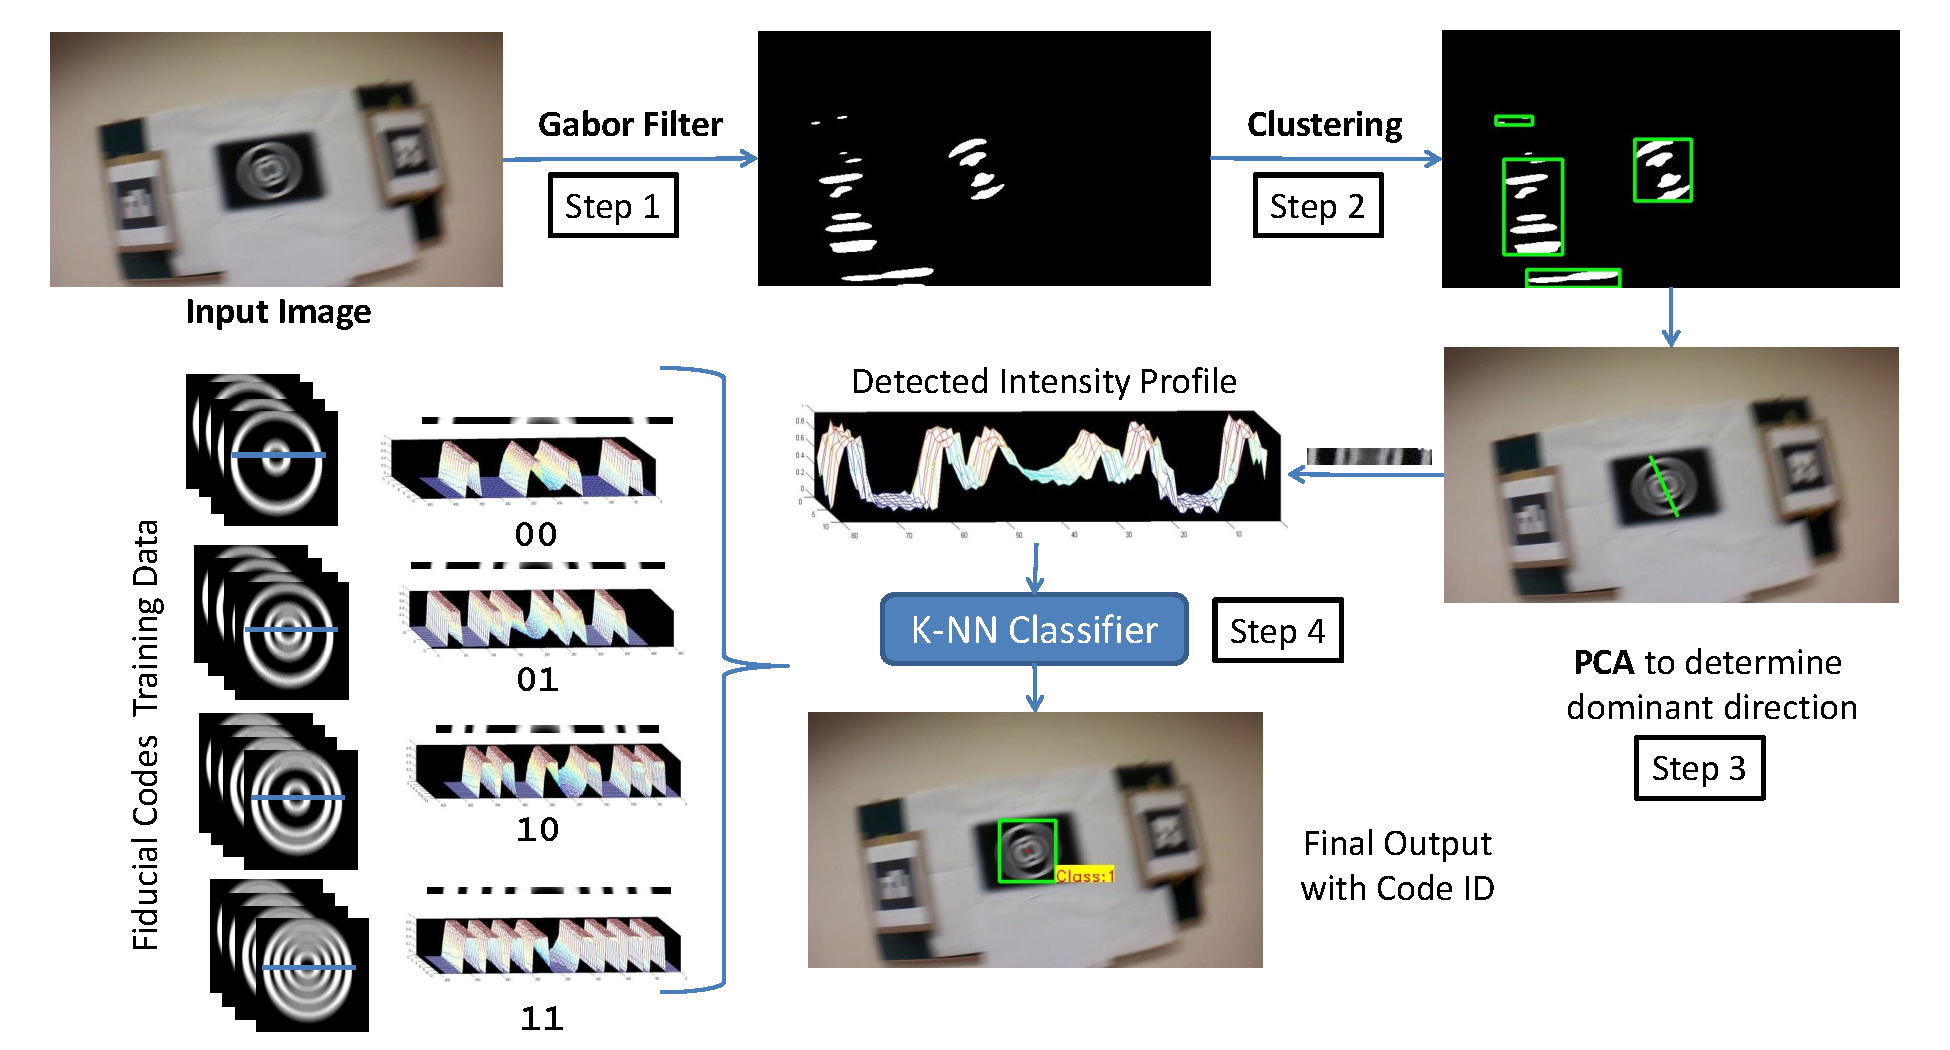
\includegraphics[width=0.8\linewidth]{figures/fiducial/overall_flow.pdf}
  \caption[Overall Workflow]{An overview of our algorithm.
    The four step process includes (Step 1) Filtering,
    (Step 2) Component clustering, (Step 3) Dominant direction determination
    and (Step 4) Classification using prior training data.}
  \label{fig:overall_flow}
\end{figure*}

%\noindent Details of each of the steps are as follows:\\
\textbf{Gabor filter:}~~A 2D Gabor filter is a Gaussian kernel function
modulated by a sinusoidal plane wave~\cite{Kruizinga:2002}. It is used to find
high gradient patches. In our case, it is used to detect portions
of the circular fiducials that were not affected by the blur.
We applied the Gabor filter in eight
different orientations ($\theta = 0, 45, 90, \ldots, 225, 270, 315$).  The
following parameters were used for creating each Gabor kernel: $\lambda$ (wavelength) $= 8$, $\gamma$
(aspect ratio) $= 0.5$, $\sigma$ (spread) $= 0.56\lambda$, $\psi$
(phase angle) $= 0$ (for real part), $\pi/2$ (for imaginary part).
Then $\ell^2$-norm of outputs along all orientations is calculated and finally
$\ell^2$-normalized image is thresholded with the threshold set to $0.4$ (on
a scale of zero to one).  For further details to the Gabor filter,
see~\cite{Kruizinga:2002}.
%% MBS - is the Kruizinga filter reasonable to cite?

\textbf{Clustering:}~~The binarized Gabor filter responses are
treated as a set of connected components in the image.   Clustering
is used to find components that are located in a close spatial region.  We do
this via hierarchical clustering~\cite{ALGLIB} using unweighted
average linkage with a distance threshold set to 150.

\textbf{PCA:}~~For each clustered set of components, we apply
PCA to determine the dominant direction.  This is done by examining
the orientation of the first principal component.  We then extract an
intensity profile patch in the input image along this direction as it
extends through the bounding box of the cluster. The signature of this
profile will be used to identify the code.

After finding the intensity profile, we project the pixel intensities
and record the number and width of the white-to-black transitions.  If
the number of transitions or the width of the transitions is not
consistent with what is allowable by our code, we reject the clustered
region as a potential fiducial.  Clustered components that have
allowable transitions counts and transitions with uniform widths are
further considered for classification to determine the binary code.

\textbf{Classification:}~~As mentioned above, a small image patch
containing the intensity profile of the fiducial is used to identify
which of the many fiducials might be present and is represented by a
code.  We found that a training-based method using the k nearest
neighbor (k-NN) technique gave better results than trying to find
binary code directly by determining the presence (or absence) of a ring
at particular positions in the image patch. This required
training-data which was easy to generate. A synthetic fiducial
is blurred along 36 orientations (0, 10, 20, \ldots , 350) with blur
scale set to 40, and the intensity profile along the first principal
component from every output is taken as training data for that
fiducial. Figure~\ref{fig:training_data} shows the process of
creating training data for fiducial with binary code ``01'' embedded
in it.  For a query image patch, we normalize the intensity range, and
then compare this information against the training data. The class
label from the closest top $K=5$ images in the training data is used
to label the patch.

\begin{figure}[h!]
\centering
  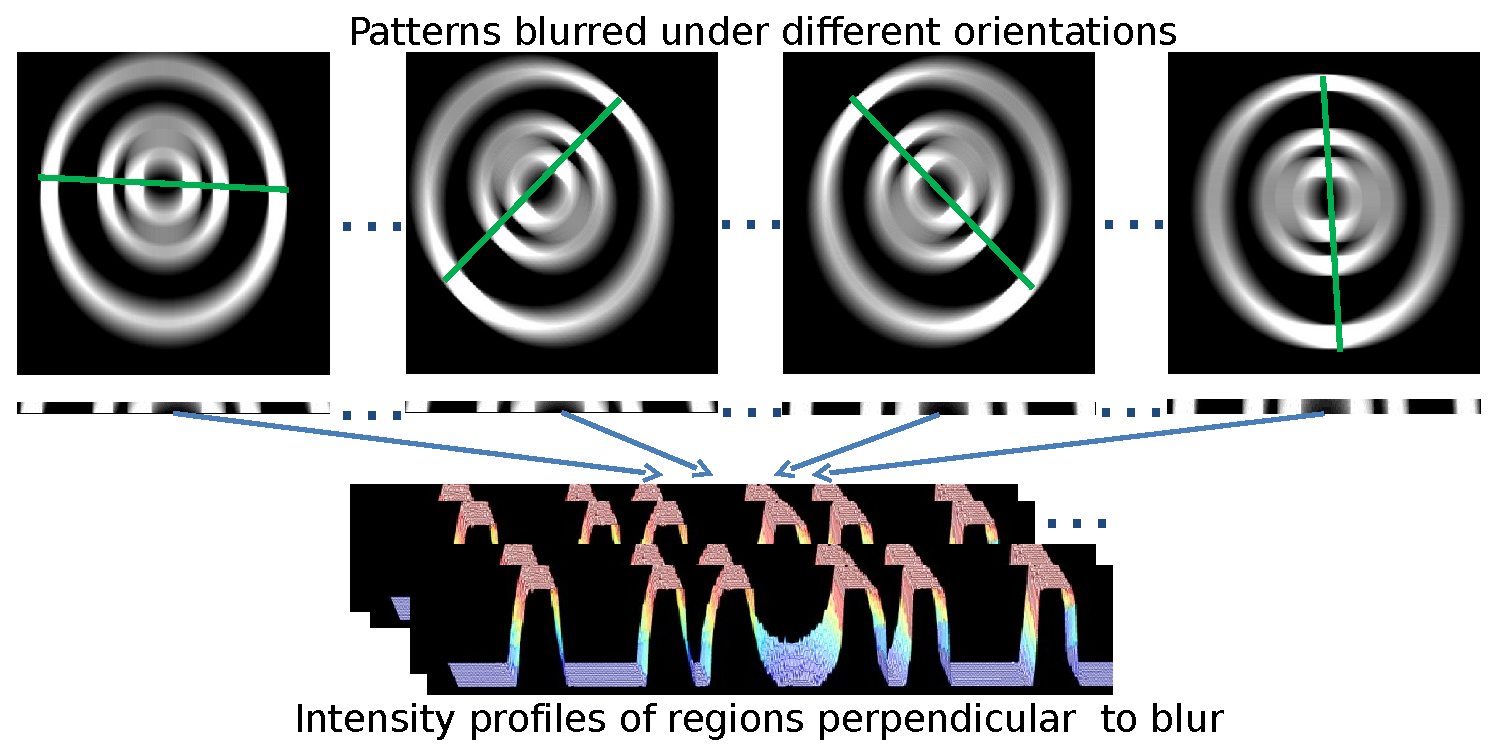
\includegraphics[width=0.95\linewidth]{figures/fiducial/training_data.pdf}
  \caption[Creation of training data for classification  for the fiducial with
  binary code ``01'']{Creating training data for the fiducial with binary code
  ``01'': The synthetic pattern is blurred along various orientations and the
  intensity profile monitored and stored. The same process is used to create
  training data for all other fiducials.}
  \label{fig:training_data}
\end{figure}

We are able to find the number of rings in the fiducial by finding
a number of transitions in the intensity profile. To increase the classification
accuracy, training data for patterns having the same number of rings are grouped
together; e.g., in two bit binary coded fiducial, training data for pattern ``01'' and ``10'' will be
grouped together. In three-bit binary coded fiducial, training data for pattern
``001'', ``010'' and ``100'' will form one group, while training data for
pattern ``110'', ``011'' and ``101'' will be in another group, and so on.
Depending on the number of detected rings in test pattern, it is matched
against the corresponding group in the training data, again using  the K-NN.
If we detect either zero rings or maximum possible
rings in the test pattern, there will be no need to do further classification, we
can classify the pattern as class 0 or the maximum class containing all 1s.

\section{Experimental Validation}

We have implemented our algorithm in C++ using the OpenCV library.
Experiments were performed on a laptop with Intel Core i7
processor(@3.4GHz) and 4GB RAM. (Please check our webpage
\url{http://meghshyam.github.io/fiducial/} for details of source code
and all datasets)
%Video clips of collected data are provided in the supplementary
%material.
% Meghshyam: Is it a desktop PC or a laptop?

Our system has been tested on several image sequences captured from an
AR Drone quadcopter.  The drone was flown indoors looking at patterns
attached to various walls. Each image sequence contains frames of
different fiducials. Some sample outputs for each fiducial
is shown in Figure~\ref{fig:out_outputs}. Our detection process takes
around 0.3 seconds which translates to slightly over three frames per
second.


\begin{figure}[h!]
\centering
  \includegraphics[width=0.4\linewidth]{figures/fiducial/output_00.jpg}
  \includegraphics[width=0.4\linewidth]{figures/fiducial/output_01.jpg}

  \includegraphics[width=0.4\linewidth]{figures/fiducial/output_10.jpg}
  \includegraphics[width=0.4\linewidth]{figures/fiducial/output_11.jpg}
  \caption[Output of our fiducial detection algorithm]{Output of our fiducial
  detection algorithm on sample images. The class label shown is the decimal
  equivalent of the binary coded fiducial.}
  \label{fig:out_outputs}
\end{figure}

Our system has also been tested on images containing multiple fiducial
patterns in the same frame. Our algorithm successfully detected
all fiducials as well as correctly classified them as shown in
Figure \ref{fig:output_all}.

\begin{figure}[ht!]
\centering
  \includegraphics[width=.45\linewidth]{figures/fiducial/output_all_2.jpg}
  \includegraphics[width=.45\linewidth]{figures/fiducial/output_test_all1.jpg}
  \caption[Result: Multiple Fiducials Detection]{Multiple fiducials in the same
  frame can be efficiently detected. }
  \label{fig:output_all}
\end{figure}

%\subsection{Comparisons}

We compare our results with the commonly used ARTag. We also compare
our results with the Blur-driven tracker (BLUT)\cite{Wu:2011}.

\subsection{Comparison with ARTag}
First, we repeat the same blur simulation experiment
(Section~\ref{sec:blurtest}) on the proposed fiducial. Specifically,
we build our blur resistant patterns at 150$\times$150 pixel
resolution and blurred them along various orientations with different
blur scales. 
%Then, we tried to detect our fiducial using a 2-bit
%patterns using algorithm presented in earlier section.

\begin{figure}[t!]
  \includegraphics[width=\linewidth]{figures/fiducial/blur_maximum.pdf}
  \caption[Result: Synthetic experiment]{On synthetic experiments, we increase
  the blur much beyond the best possible results (see Figure~\ref{fig:artag_pitag}) for
    prior methods. Even upto 65 units, the algorithm is successful.}
  \label{fig:blur_maximum}
\end{figure}

Qualitatively, we see in Figure~\ref{fig:blur_maximum} that despite of
even more blur than earlier described (50 units or more), detection is
still feasible and practical.  Quantitatively, the comparison of
recognition rate is shown in Figure~\ref{fig:recognition_rate}.
Even under more severe blur, of 65 pixels, the algorithm is
successful.  Our recognition is 100\% for all codes except the ``00''
which is undetectable after 50 pixels blur (which is still
significantly better than ARTag).  Reasons for the lower performance
when``00'' tags are present, is discussed in
Section~\ref{sec:discussion}.

\begin{figure}[h!]
\centering
\includegraphics[width=\linewidth]{figures/fiducial/recognition_rate.pdf}  
\caption[Comparison of recognition rate of fiducials]{Comparison of recognition
rate of fiducials.  The proposed fiducial handsomely outperforms prior methods.}
\label{fig:recognition_rate}
\end{figure}


We also performed analysis to detect how accurately the center of the
blur pattern can be localized under blur.  To do this, we have
simulated data along different blur orientations for all patterns over
eight different blur scales (30 to 65 with the step size of 5). Values for
the localization of the pattern ``00'' after blur with 50 pixels is
omitted since the pattern cannot be detected. From
Table~\ref{tab:blur_angle_center}, it can be clearly seen that the 
mean error in locating center by our algorithm is within approximate 3
pixels, or 3\% of the diameter of the fiducial.

\begin{table}[h!]
  \centering
  \begin{tabularx}{0.6\linewidth}{|Y|Y|}
    \cline{1-2}
    \footnotesize{Blur} & \footnotesize{Mean($\pm$std) error}  \\
    \footnotesize{angle} & \footnotesize{(in pixels)}  \\
    \cline{1-2}
    \footnotesize{0} & \footnotesize{1.33 $\pm$ 0.40}  \\
    \footnotesize{22} & \footnotesize{2.42 $\pm$ 1.05} \\
    \footnotesize{45} & \footnotesize{1.46 $\pm$ 0.65}  \\
    \footnotesize{67} & \footnotesize{2.39 $\pm$ 1.28}  \\
    \footnotesize{90} & \footnotesize{1.83 $\pm$ 0.25}  \\
    \cline{1-2}
  \end{tabularx}
    \caption{Center localization error.
      Error is computed for various blur angles over various scales.}
    \label{tab:blur_angle_center}
\end{table}



\begin{comment}
\begin{figure*}
\centering
\begin{tabular}{c|c}
\begin{subfigure}[b]{0.45\linewidth}
\centering
\includegraphics[width=\linewidth]{figures/fiducial/recognition_rate.pdf}
\caption{Comparison of recognition rate of fiducials}
\label{fig:recognition_rate}
\end{subfigure}
&
\begin{subfigure}[b]{0.25\linewidth}
\centering
\begin{tabularx}{\textwidth}{|c|Y|}
\cline{1-2}
\footnotesize{Blur} & \footnotesize{Mean($\pm$std) error}  \\
\footnotesize{angle} & \footnotesize{(in pixels)}  \\
\cline{1-2}
\footnotesize{0} & \footnotesize{1.33 $\pm$ 0.40}  \\
\footnotesize{22} & \footnotesize{2.42 $\pm$ 1.05} \\
\footnotesize{45} & \footnotesize{1.46 $\pm$ 0.65}  \\
\footnotesize{67} & \footnotesize{2.39 $\pm$ 1.28}  \\
\footnotesize{90} & \footnotesize{1.83 $\pm$ 0.25}  \\
\cline{1-2}
\end{tabularx}
\caption{Center localization error}
\label{tab:blur_angle_center}
\end{subfigure}
\end{tabular}
\caption{(a): Comparison of recognition rate of the ARTag and our fiducials on
blur simulated data at various blur scales. It can be seen that except for the
fiducial with binary code ``00'', our fiducials are recognized all times.
(b): Table showing the mean error and standard deviation of the localized fiducial center
versus the ground truth.  Error is computed for various blur angles over
different blur scales.}
\label{fig:simulated_blur}
\end{figure*}
\end{comment}

\subsection{Real Data}

We also compared results on the recorded feed using the AR Drone
quadcopter. In our experimental setup, we have placed two ARTags in
the scene along with our fiducial to compare the resilience of blur by
each fiducial type. We have used ar\_track\_alvar, ROS Wrapper for the
ALVAR library~\cite{ros_alvar}, to detect the ARTags from the stream
captured with the quadcopter camera. In each test dataset, we have
used different two-bit binary coded fiducial and recorded video of
around two minute duration (i.e., around 1000 frames).  The quadcopter
was flown in a routine manner in the room with its camera facing the
wall. The comparison of the recognition
rate is shown in Table~\ref{tab:recognition_accuracy}. Recognition
rate of our fiducials ranges from 86.5\% to 94.1\%, while the ARTag is
60.3\% to 65.6\%.  Classification accuracy of all fiducials (ARTag as
well as ours) was approximately 100\%, i.e., when tags were detected
they were the correct fiducials and not other objects in the scene.

\begin{table}[t!]
  \centering
  \begin{tabularx}{\linewidth}{|c|Y|Y|Y|Y|}
    \cline{1-5}
    \multirow{2}{*}{Test \#} & {Number}
    &{Binary} &\multicolumn{2}{c|}{Recognition Rate (\%)} \\
    \cline{4-5} & {of frames}& {Code}& ARTag & Our Fiducial \\\cline{1-5}
    1 & 1205 & 00 &  65.6 & 86.5  \\ \cline{1-5}
    2 & 1047 & 01 &  61.9 & 94.1  \\ \cline{1-5}
    3 & 1102 & 10 &  62.4 & 92.74 \\ \cline{1-5}
    4 & 1081 & 11 &  60.3 & 93.54  \\ \cline{1-5}
  \end{tabularx}
  \caption[Comparison of Recognition Rate: Real Data]{ 
  \label{tab:recognition_accuracy} Recognition rate of ARTag and proposed fiducials on real
    data captured through AR Drone. Each row shows analysis of a test
    dataset captured for our fiducial with different binary codes embedded in it.
    Each dataset has around 1000 frames captured representing roughly two
    minutes of video.} 
\end{table}

In another setup, we arranged our fiducials on four sides of a box and
revolved the quadcopter around the box (See  \cite{video}).
Later, we repeated the process by replacing our fiducial by ARTags. Figure~\ref{fig:setup} shows some
frames from this sequence as well as the performance of both
fiducials. The overall detection rate of our tags is 90\% while that
of ARTags is only around 60\%.

\begin{figure*}[hb!]
\begin{subfigure}[b]{.19\textwidth}
\includegraphics[width=\linewidth]{figures/fiducial/setup_artag/output_79.jpg}
\end{subfigure}
\begin{subfigure}[b]{.19\textwidth}
\includegraphics[width=\linewidth]{figures/fiducial/setup_artag/output_150.jpg}
\end{subfigure}
\begin{subfigure}[b]{.19\textwidth}
\includegraphics[width=\linewidth]{figures/fiducial/setup_artag/output_194.jpg}
\end{subfigure}
\begin{subfigure}[b]{.19\textwidth}
\includegraphics[width=\linewidth]{figures/fiducial/setup_artag/output_339.jpg}
\end{subfigure}
\begin{subfigure}[b]{.19\textwidth}
\includegraphics[width=\linewidth]{figures/fiducial/setup_artag/output_480.jpg}
\end{subfigure}\\
\begin{subfigure}[b]{.19\textwidth}
\includegraphics[width=\linewidth]{figures/fiducial/setup_our/output_6/output_514.jpg}
\end{subfigure}
\begin{subfigure}[b]{.19\textwidth}
\includegraphics[width=\linewidth]{figures/fiducial/setup_our/output_2/output_64.jpg}
\end{subfigure}
\begin{subfigure}[b]{.19\textwidth}
\includegraphics[width=\linewidth]{figures/fiducial/setup_our/output_2/output_35.jpg}
\end{subfigure}
\begin{subfigure}[b]{.19\textwidth}
\includegraphics[width=\linewidth]{figures/fiducial/setup_our/output_2/output_330.jpg}
\end{subfigure}
\begin{subfigure}[b]{.19\textwidth}
\includegraphics[width=\linewidth]{figures/fiducial/setup_our/output_6/output_943.jpg}
\end{subfigure}\\
\begin{subfigure}[b]{\textwidth}
\includegraphics[width=\linewidth]{figures/fiducial/compare_detection.jpg}
\end{subfigure}
\caption[Comparison of ARTag and our fiducial when quadcopter is
  revolving around our setup]{Comparison of ARTag and our fiducial when quadcopter is
  revolving around our setup. 
\textbf{Top} ARTags are not detected, shown by an absence of green rectangles. \textbf{Middle} In
similar conditions, proposed fiducials are successfully
detected. The overall detection rate of proposed
fiducials is 90\% while that of ARTags is around 60\%. 
\textbf{Bottom Rows} Time view of detection. ARTag is ``choppy'' with
frequent losses, while the proposed fiducial (extreme bottom) is
``up'' almost all the 
time.}
\label{fig:setup}
\end{figure*}


\subsubsection{Comparison with BLUT}

We also compare our approach with tracking designed for blurred input
scenes.  We have used four image sequences (consisting of around 1000
frames each). Each sequence contains different fiducials so that we
are able to contrast the performance of BLUT~\cite{Wu:2011} with the
proposed method.  From the images in the top rows of
Figure~\ref{fig:BLUT_compare_00}--\ref{fig:BLUT_compare_11},
we can see that BLUT is able to track the fiducial when the position
of fiducial does not change too much in successive frames. Also, it
can be seen that once BLUT loses track of the fiducial, it is not
able to recover. Since our approach detects the code in each frame,
large changes in the pattern's position is not an issue.  Our fiducial
detection results are also shown in
Figure~\ref{fig:BLUT_compare_00}--\ref{fig:BLUT_compare_11}.

We have also found that even if we reset the BLUT tracker after it
loses track, the tracker will once again malfunction after around 100
frames (approximately within 6 seconds). When we checked the timestamp
data from image header captured through the AR Drone, we found that,
there was a difference of 0.14 seconds between two successive frames
indicating the dropping of a video frame (normal 30fps should have a gap
of 0.033 seconds). Also, there were around 50 instances in 1000 frames
where the timestamp difference between two successive frames was
greater than 0.1 seconds. As such, it appears one of the main culprits
causing the BLUT tracker to fail is the dropping of frames combined
with the unstable motion of quadcopter, resulting in large discrepancies in
the  position of the fiducial between successive frames.

\begin{figure*}[t!]
\begin{subfigure}[b]{.19\textwidth}
\includegraphics[width=\linewidth]{figures/fiducial/BLUT_output_00/2.jpg}
\end{subfigure}
\begin{subfigure}[b]{.19\textwidth}
\includegraphics[width=\linewidth]{figures/fiducial/BLUT_output_00/3.jpg}
\end{subfigure}
\begin{subfigure}[b]{.19\textwidth}
\includegraphics[width=\linewidth]{figures/fiducial/BLUT_output_00/4.jpg}
\end{subfigure}
\begin{subfigure}[b]{.19\textwidth}
\includegraphics[width=\linewidth]{figures/fiducial/BLUT_output_00/5.jpg}
\end{subfigure}
\begin{subfigure}[b]{.19\textwidth}
\includegraphics[width=\linewidth]{figures/fiducial/BLUT_output_00/6.jpg}
\end{subfigure}\\
\begin{subfigure}[b]{.19\textwidth}
\includegraphics[width=\linewidth]{figures/fiducial/BLUT_input_00/output2.jpg}
\end{subfigure}
\begin{subfigure}[b]{.19\textwidth}
\includegraphics[width=\linewidth]{figures/fiducial/BLUT_input_00/output3.jpg}
\end{subfigure}
\begin{subfigure}[b]{.19\textwidth}
\includegraphics[width=\linewidth]{figures/fiducial/BLUT_input_00/output4.jpg}
\end{subfigure}
\begin{subfigure}[b]{.19\textwidth}
\includegraphics[width=\linewidth]{figures/fiducial/BLUT_input_00/output5.jpg}
\end{subfigure}
\begin{subfigure}[b]{.19\textwidth}
\includegraphics[width=\linewidth]{figures/fiducial/BLUT_input_00/output6.jpg}
\end{subfigure}
\caption[Output of BLUT on ARTag and our fiducial with code
``00'']{\textbf{Top:} Output of BLUT~\cite{Wu:2011}.
\textbf{Bottom:} Output of our algorithm on the same image 
  sequence. BLUT is able to track the fiducial till the third frame,
  but from the fourth frame onwards, BLUT loses track. In the first
  three frames, the size of the  bounding box is low, but in the fourth
  and the fifth frame it is large, indicating a sudden forward movement
  of the quadcopter.} 
\label{fig:BLUT_compare_00}
\end{figure*}

\begin{figure*}[ht!]
\begin{subfigure}[b]{.19\textwidth}
\includegraphics[width=\linewidth]{figures/fiducial/BLUT_output_01/11.jpg}
\end{subfigure}
\begin{subfigure}[b]{.19\textwidth}
\includegraphics[width=\linewidth]{figures/fiducial/BLUT_output_01/12.jpg}
\end{subfigure}
\begin{subfigure}[b]{.19\textwidth}
\includegraphics[width=\linewidth]{figures/fiducial/BLUT_output_01/13.jpg}
\end{subfigure}
\begin{subfigure}[b]{.19\textwidth}
\includegraphics[width=\linewidth]{figures/fiducial/BLUT_output_01/14.jpg}
\end{subfigure}
\begin{subfigure}[b]{.19\textwidth}
\includegraphics[width=\linewidth]{figures/fiducial/BLUT_output_01/15.jpg}
\end{subfigure}\\
\begin{subfigure}[b]{.19\textwidth}
\includegraphics[width=\linewidth]{figures/fiducial/BLUT_input_01/output11.jpg}
\end{subfigure}
\begin{subfigure}[b]{.19\textwidth}
\includegraphics[width=\linewidth]{figures/fiducial/BLUT_input_01/output12.jpg}
\end{subfigure}
\begin{subfigure}[b]{.19\textwidth}
\includegraphics[width=\linewidth]{figures/fiducial/BLUT_input_01/output13.jpg}
\end{subfigure}
\begin{subfigure}[b]{.19\textwidth}
\includegraphics[width=\linewidth]{figures/fiducial/BLUT_input_01/output14.jpg}
\end{subfigure}
\begin{subfigure}[b]{.19\textwidth}
\includegraphics[width=\linewidth]{figures/fiducial/BLUT_input_01/output15.jpg}
\end{subfigure}
\caption[Output of BLUT on ARTag and our fiducial with  code ``01'']{{\bf Top:}
Output of BLUT~\cite{Wu:2011} on a sequence containing the ``01'' binary coded fiducial. {\bf Bottom:} Output of our
algorithm on the same image 
sequence. BLUT loses  track from the third frame onwards.}
\label{fig:BLUT_compare_01}
\end{figure*}

\begin{figure*}[ht!]
\begin{subfigure}[b]{.19\textwidth}
\includegraphics[width=\linewidth]{figures/fiducial/BLUT_output_10/1.jpg}
\end{subfigure}
\begin{subfigure}[b]{.19\textwidth}
\includegraphics[width=\linewidth]{figures/fiducial/BLUT_output_10/2.jpg}
\end{subfigure}
\begin{subfigure}[b]{.19\textwidth}
\includegraphics[width=\linewidth]{figures/fiducial/BLUT_output_10/3.jpg}
\end{subfigure}
\begin{subfigure}[b]{.19\textwidth}
\includegraphics[width=\linewidth]{figures/fiducial/BLUT_output_10/4.jpg}
\end{subfigure}
\begin{subfigure}[b]{.19\textwidth}
\includegraphics[width=\linewidth]{figures/fiducial/BLUT_output_10/5.jpg}
\end{subfigure}\\
\begin{subfigure}[b]{.19\textwidth}
\includegraphics[width=\linewidth]{figures/fiducial/BLUT_input_10/output1.jpg}
\end{subfigure}
\begin{subfigure}[b]{.19\textwidth}
\includegraphics[width=\linewidth]{figures/fiducial/BLUT_input_10/output2.jpg}
\end{subfigure}
\begin{subfigure}[b]{.19\textwidth}
\includegraphics[width=\linewidth]{figures/fiducial/BLUT_input_10/output3.jpg}
\end{subfigure}
\begin{subfigure}[b]{.19\textwidth}
\includegraphics[width=\linewidth]{figures/fiducial/BLUT_input_10/output4.jpg}
\end{subfigure}
\begin{subfigure}[b]{.19\textwidth}
\includegraphics[width=\linewidth]{figures/fiducial/BLUT_input_10/output5.jpg}
\end{subfigure}
\caption[Output of BLUT on ARTag and our fiducial with  code ``10'']{Top: Output
of BLUT~\cite{Wu:2011} on sample image sequence containing ``10'' binary coded fiducial. Bottom: Output of our algorithm on the same image
sequence. From the second frame, BLUT loses track.}
\label{fig:BLUT_compare_10}
\end{figure*}

\begin{figure*}[ht!]
\begin{subfigure}[b]{.19\textwidth}
\includegraphics[width=\linewidth]{figures/fiducial/BLUT_output_11/2.jpg}
\end{subfigure}
\begin{subfigure}[b]{.19\textwidth}
\includegraphics[width=\linewidth]{figures/fiducial/BLUT_output_11/3.jpg}
\end{subfigure}
\begin{subfigure}[b]{.19\textwidth}
\includegraphics[width=\linewidth]{figures/fiducial/BLUT_output_11/4.jpg}
\end{subfigure}
\begin{subfigure}[b]{.19\textwidth}
\includegraphics[width=\linewidth]{figures/fiducial/BLUT_output_11/5.jpg}
\end{subfigure}
\begin{subfigure}[b]{.19\textwidth}
\includegraphics[width=\linewidth]{figures/fiducial/BLUT_output_11/6.jpg}
\end{subfigure}\\
\begin{subfigure}[b]{.19\textwidth}
\includegraphics[width=\linewidth]{figures/fiducial/BLUT_input_11/output2.jpg}
\end{subfigure}
\begin{subfigure}[b]{.19\textwidth}
\includegraphics[width=\linewidth]{figures/fiducial/BLUT_input_11/output3.jpg}
\end{subfigure}
\begin{subfigure}[b]{.19\textwidth}
\includegraphics[width=\linewidth]{figures/fiducial/BLUT_input_11/output4.jpg}
\end{subfigure}
\begin{subfigure}[b]{.19\textwidth}
\includegraphics[width=\linewidth]{figures/fiducial/BLUT_input_11/output5.jpg}
\end{subfigure}
\begin{subfigure}[b]{.19\textwidth}
\includegraphics[width=\linewidth]{figures/fiducial/BLUT_input_11/output6.jpg}
\end{subfigure}
\caption[Output of BLUT on ARTag and our fiducial with  code ``11'']{Top: Output
of BLUT~\cite{Wu:2011} on sample image sequence containing ``11'' binary coded fiducial. Bottom: Output of our algorithm on the same image
sequence. BLUT lost the track from third frame. There is sudden reversal of
direction from the quadcopter in the third frame. In first two frames, the quadcopter was
going up, but suddenly moved down.}
\label{fig:BLUT_compare_11}
\end{figure*}


\section{Identification of quadcopter using fiducials}
Multiple quadcopters can be used for applications such as inspection of dams,
bridges. Quadcopters need to identify themselves accurately so that
effective collaboration among them can happen. E.g., Consider there are two
quadcopters covering a large plane virtually divided in two parts. We would like  
the quadcopter on the left side of a plane to cover left part of the scene. Similarly, the 
quadcopter on right will cover the right part. Both quadcopters need to identify that there
is another quadcopter and collaborate with each other to complete their respective 
tasks efficiently.

\begin{figure}[hb!]
  \includegraphics[width=\linewidth]{figures/fiducial/fiducialOnDrone}
  \caption[Fiducials on Quadcopter]{Identification of sides of quadcopter using
  fiducials. (a) shows our distinct fiducials put on two sides of
  quadcopter.(b) shows fiducial with binary code ``11"( class 3) being detected
  from one side while (c) shows fiducial with binary code ``10"(class 2) being
  detected from other side.}
  \label{fig:fiducialOnDrone}
\end{figure}

Tracking of objects in motion is a challenging task as shown in
Section~\ref{sec:intro}. Hence, we propose to use our fiducials on the
quadcopter itself. We have put our two-bit fiducials on two sides of the
quadcopter as shown in Figure~\ref{fig:fiducialOnDrone}(a). 
Currently, we have used another camera to capture this moving quadcopter.
However, in practice, we can use a quadcopter to capture another quadcopter.
Figure~\ref{fig:fiducialOnDrone}(b) and (c) shows the detection of
and classification of fiducials from two sides. As each fiducial carry a
unique code, we can accurately tell that which side of the quadcopter we are
looking at.

\section{Discussion and Limitations}\label{sec:discussion}

We have demonstrated the effectiveness of our blur invariant fiducial
both on synthetic data, and on real video clips captured from a quadcopter.
Our approach obtains a recognition rate of 86\%--95\% 
in real scenes compared to existing methods that average around
64\%.  We discuss some limitations of our approach in this section.
%\noindent\textbf{Processing Time}~~

Our  current processing time (0.3 seconds per frame) does not provide
real-time performance.  As such, we envision the method will be used in an
offline manner for performing analysis of flight paths. Code profiling revealed
that the Gabor filtering along the eight directions takes most of the time
(0.03 -- 0.04 seconds per orientation).  Either an improved Gabor filter scheme
is required or an alternative strategy for detection is required.
%\noindent\textbf{False Negatives}~~

We found that sometimes our detection algorithm fails to recognize the
``00'' fiducial, when there is a severe blur.  This is because when there
is too much blur, the innermost ring's response in the Gabor output is
too low and not detected properly.  This problem can be resolved by
increasing the radius of the innermost ring to reduce the effect of blur
on the innermost ring.
%\noindent\textbf{Pose Estimation}~~

We note that other markers are able to give full pose estimation after
detection.  However, we are only able to reliably detect the center
point and therefore cannot estimate pose.  Of course, if four markers
were used in a known order, pose could be estimated. The current
resolution of the onboard camera is a significant  hurdle to clear before we
can effectively use multiple markers in each scene.
%\noindent\textbf{Number of Fiducials}~~

In terms of numbers of fiducials, we are able to generate fewer markers
than ARTag. Many applications in robotics (e.g., quadcopter navigation)
may not require simultaneous use of a large number of fiducials.  Most
of the time, it is sufficient to have 4-6 different
fiducials. Nevertheless, we may be able to generate a larger number of
fiducials by using color backgrounds. This is an area of interest for
further research.

\section{Concluding remarks}
Quadcopters are subject to quick and unstable motions that can cause
significant motion blur in the captured images. This severely affects
the detection rate of existing fiducials. We proposed the
design of a fiducial that is resistant to motion blur. Our design of
contrasting concentric rings is based on the observation that the
direction perpendicular to the motion blur direction will be
unaffected by the blur and therefore still be recognizable. We have
shown through experimental validation that our fiducial will work
under large amounts of motion blur and can significantly outperform
existing fiducials under this scenario.

Our fiducials are also of great help in collaboration among multiple
quadcopters for tracking. We have demonstrated that using our fiducials we
can tell from which side of the quadcopter we are gazing.

%\chapter[Stagnant Water Detection]{Stagnant Water Detection through Quadcopter}
Dengue~\cite{WHO15Dengue} is a troublesome debilating disease with no
known preventing vaccine, or cure. Doctors advocate that the best way
to avoid this disease is to avoid being bitten by mosquitoes which is
virtually an impossibility for many people in India.  The greatest
risk of contracting dengue (pronounced DENgee) is in the Indian
subcontinent.  

Technology is a must in tackling this situation.  The risk of disease
can be reduced by using insect repellents. In our institute, the
common method has been the spraying of insecticides.  Reports in the
media~\cite{china} indicate that China has flooded a small island
releasing half a million sterile mosquitoes to dominate the potent
mosquitoes. Such measures have unknown and unforeseen environmental
impact on the eco-system. Regardless, researchers are convinced that
there is no one single magic bullet to tackle the disease. 

Our work, started prior to the announcement of ``Project
Premonition,'' is similar to that of \cite{Microsoft15}.  Instead of
attempting to destroy the mosquito, we seek to detect the reason for
the increased outbreak, especially in urban areas.  Our work complements that
of \cite{Microsoft15} --- the goal in \cite{Microsoft15} is to ``catch wild
mosquitoes'' (typically in the outfield) by creating novel mosquito traps, and
then to test mosquitoes for pathogens. New traps are placed by drones, and
retrieved by drones. In contrast, we emphasize the need for
identifying the location of these traps.  

One of the major reasons behind the growth of mosquitoes is the
continuous existence of \emph{water puddles} around residencies in
urban India.  The virus is carried by mosquitoes, and these breed in
stagnant water. \emph{Can we detect stagnant water?}  When we surveyed
terraces (Fig.~\ref{fig:stagnantTeaser}) and ``chajjas'' of various buildings in
our institute, we found split AC air conditioners dumping condensed
water. Such areas can be surveyed using autonomous quadcopters.

\begin{figure}[h!]
\centering
\includegraphics[width=\linewidth]{figures/stagnantWater/teaser.pdf}
\caption[Overview]{(a) Our hovering quadcopter (b) A
typical rooftop on campus (c) Earlier method \cite{rankin2004daytime} applied, and
  output marked in red (d) Our output. Notice (marked as black oval in
  (c)) that \cite{rankin2004daytime} confuses non-puddle patches as puddle.
  Also, note (marked as green ellipse in (d)) that \cite{rankin2004daytime} is
  not able to detect puddle which are dark.}
\label{fig:stagnantTeaser}  
\end{figure}

\textbf{Contributions:} The scientific challenge in identifying water
is that it is specular in nature, and acts like a mirror.  Water is
like a chameleon changing its color depending on the environment, and
there is no easy way of saying ``this is water'' based on its
appearance. In this work, we propose the use of an old paradigm of
optical flow for the novel application to stagnant water detection.
We couple it with a modern SVM-based method of classification.

\textbf{Related Work} The method in ~\cite{santana12} for detection of
water relies on the chaotic nature of water's dynamic texture to
exploit a measure of entropy over the trajectories obtained from
optical flow trackers over several frames. \cite{zhang10} has
introduced a descriptor which is tolerant to the flip transformation
and even non-rigid distortions, such as ripple effects.  \emph{These
  methods and others in the literature focus on the turbulent aspects
  of water}, largely absent in our application that focuses on
stagnant water.  Our method is closest to that of Rankin et
al.~\cite{rankin2004daytime, rankin11} who have implemented a rule-based water
detector based on sky reflections.  These rules are established
based on an analysis of images captured in wide-open areas on
cross-country terrain. Not only do we have new methods, \emph{our
datasets are captured in urban areas using a quadcopter and thus these
rules seem unlikely to be readily applicable.}

\section{Methodology}  Our method is based on a combination of color
based method with an optical flow based method.  We establish the
need for the combination in the first two subsections.

\subsection{Appearance-based Detection }

\begin{figure}[h!]
  \centering
  \includegraphics[width=0.4\linewidth]{figures/stagnantWater/IMG_PAIR_27_1.jpg} \hfill
  \includegraphics[width=0.4\linewidth]{figures/stagnantWater/IMG_PAIR_27_1_H.jpg} 

  \includegraphics[width=0.4\linewidth]{figures/stagnantWater/IMG_PAIR_27_1_S.jpg} \hfill
  \includegraphics[width=0.4\linewidth]{figures/stagnantWater/IMG_PAIR_27_1_V.jpg}
  \caption[HSV Components]{An image (top left) and the HSV components.  The
  puddle has low saturation (bottom left) but high intensity (bottom right).
    The hue is indeterminable and is based on the environment.}
  \label{fig:HSV}
\end{figure}

Under ambient lighting conditions, puddle areas display high
brightness and low saturation as can be seen in
Fig.~\ref{fig:HSV}. Features based on these are fed to an SVM
classifier. Training an SVM is a labour intensive task.  To reduce the
effort, we have developed a tool shown in
Fig.~\ref{fig:training}. 
%This tool, and other data, will be released in the public domain.

% that
% capture this information locally could be used for puddle
% detection. Hence, considering a square image patch of small side
% dimension, $n$, a novel feature is used that performs the following
% steps:
% \begin{enumerate}
% \item Image is transformed from RGB color domain to HSV color space.
% \item Histogram for each channel having k bins is constructed
% \item The histogram values for three channels are concatenated to form a vector
% of length $3k$.
% \end{enumerate}
 
% Here, to capture sufficient statistics as well as constrain the feature size,
% number of bins, k = 64 is chosen, such that each bin contains 4 consecutive gray
% levels. Also, the side of square patch is taken as $n = 50$ to capture local
% characteristics.

% The given feature is used to train a Support Vector Machine(SVM) using a
% dataset of positively and negatively marked puddle patches. The
% positively-labelled as well as negatively-labelled patches are manually marked
% from a grid of size $m$ pixels overlaid on frames captured using quadcopter.
% Since RBF kernels have been useful to efficiently detect
% textures~\cite{Chapelle99}, it has been used for the given classifier. In our
% experiments, values of $m = 16$ is used.


% We have created a tool to select training data for the classifier. In this tool,
% image will be shown in grid fashion with block size of $50  \times 50$. 
% User will be enabled to draw contour over the desired region (puddle or
% non-puddle). The blocks enclosed by the contour will be selected. Additionally
% user may select additionally select blocks or deselect the selected blocks. The
% process is 

\begin{figure}[h!]
  \centering
  \includegraphics[width=0.9\linewidth]{figures/stagnantWater/trainingData.pdf}
  \caption[Creation of Training Data]{The process for creation of training data.
  The user selects the stagnant water area by drawing a contour to produce `positive'
    and `negative'  data.}
  \label{fig:training}
\end{figure}

\textbf{Failure of SVM-based methods:} The SVM detector is good at
detecting regions of sky reflected off a puddle.  In the HSV color
space, these regions have low saturation (S) and high brightness (V)
values, and are picked up with high reliability by the HSV histogram
feature based SVM detector. However, false negatives are also produced
since other reflected regions such as trees, buildings, etc. are
usually classified as non-puddle regions as many of these
characteristics is shared by negative images in the training data set.


\subsection{Optical flow based Detection}
Fortunately our images are captured by a moving quadcopter.  The
optical flow measures apparent motion of objects in a scene caused by
relative motion between camera and object. The magnitude of the
optical flow is high for objects that are close in comparison to
objects at a distance.  Fig.~\ref{fig:optical_flow} shows the
magnitude of optical flow calculated from two images.

\begin{figure}[h!]
  \centering
  \includegraphics[width=0.32\linewidth]{figures/stagnantWater/IMG_PAIR_27_1.jpg} \hfill
  \includegraphics[width=0.32\linewidth]{figures/stagnantWater/IMG_PAIR_27_2.jpg} \hfill
  \includegraphics[width=0.32\linewidth]{figures/stagnantWater/IMG_PAIR_27_optical_flow.jpg}
  \caption[Sample Optical Flow]{Optical Flow. Left, Middle: Frames taken from
  positions which are $d$ units apart in 3D world. $ 0.01 \leq d \leq 0.1$. Right:
    Magnitude of optical flow. We observe that the magnitude of optical
    flow in the reflective parts of the puddle is relatively low.}
  \label{fig:optical_flow}
\end{figure}

A recent thesis \cite{Liu11Thesis} has one of the state of the art
algorithm for optical flow. One requirement is the need for
spatio-temporal smoothness constraint which can be challenging because
of the jerky movement of the UAV.  To resolve this, we use the
Inertial Measurement Unit (IMU) data available on the quadcopter to
synchronize positional information with the video sequence captured by
quadcopter. In short, we select the frame pair which are spatially the
closest, among a set of competing temporally adjacent frames.

\textbf{Failure of optical flow:} Optical flow is essentially being
used in a depth from parallax mode to exploit the fact that still
puddles behave like mirrors. The scenery reflected by such puddles is
usually at a much greater depth than the immediate surroundings of the
puddle.  Optical flow is largely independent of hue and saturation.
For the same reason, however, optical flow as a means of detecting
puddles will fail to report true positives when the object that is
being reflected is close by. In such cases, the saturation and
intensity values are useful.

Yet another reason for the failure for the optical flow is the
inability to distinguish true ``far away'' regions versus imagined far
away regions due to the mirror-like properties of water.  To handle
these false positives, we devise a horizon mask based on the principle
that water flows down.

\subsection{Combined approach}
\textbf{Horizon Mask:} The change in depth for far-away scenes as well
as their reflections on puddle, in consecutive frames, are hard to
distinguish. In previous work \cite{rankin11} such issues are avoided
by discarding a fixed-portion of image corresponding to far-off
regions, enforced by constrained input capture method. Due to
inapplicability of such constraints in the comparatively agile input
capture conditions of quadcopter, features derived from urban
environment are utilized for finding plausible puddle regions. In
urban setting, the high availability of structures in surroundings,
having distinctly flat surfaces and rectilinear silhouettes, enables
use of edge-detection based methods to bound planar regions that can
contain puddle. Applying the Hough transform with calibrated
parameters followed by length-based selection of lines detected, a
upper boundary for puddle region called `Horizon' is found. The
Horizon is in turn used to create a binary mask to be applied to local
scores from other techniques before normalization.


\begin{figure}[h!]
  \centering
  \includegraphics[width=0.9\linewidth]{figures/stagnantWater/overall_workflow.pdf}
  \caption{Overall architecture.}
  \label{fig:workflow}
\end{figure}

These observations suggested a novel combined approach as sketched
in Fig.~\ref{fig:workflow}.


% As illustrated in Figure~\ref{fig:workflow}, first we select coherent
% spatio temporal frames in pairs and obtain optical flow scores and
% SVM scores.  


% The SVM scores are obtained from classifier correspond to each patch of size, m
% ( m = 16 as mentioned in section), while for computational efficiency, optical
% flow is performed on frames downsampled to half of the original dimensions.
% But, to obtain a combined estimate based on both techniques, scores for a
% common patch size are necessary. Hence, the optical flow scores are divided
% into a grid of size $m/2$ pixels, each sub-patch of which are averaged to
% obtain the final optical flow score.

% The combined score obtained from optical flow and SVM classifier provides a
% probabilistic estimate of corresponding patch belonging a puddle. But, in order
% to include contribution towards the estimate based on neighborhood
% information, a sequence of morphological operations are applied on the
% combined score. From the resulting score, a mask denoting puddle region is
% obtained by thresholding based on statistical parameters.

\section{Experiments and Results}

All our experiments have been completed with the inexpensive consumer
quadcopter called Parrot's AR Drone. We remark that one should not
compare expensive military grade drones with such inexpensive drones.
For the purpose of showing the efficacy of this work, we also took a
picture of the scene from a distance with a 5 mega-pixel camera for
the reader to better understand the scene.  We covered urban places
such as terraces, constructions sites, building backyards,
pumping stations, and so on.  We have captured around eight different
types of datasets, each having around two-three minutes of video
(around 3000 frames each). 

%Due to page restriction, and file size
%restriction, in this paper, as well as in the
%supplementary material, we have shown only representative frames from
%captured videos. Frames not having any stagnant water are not shown. 
% Please see
% the supplementary material for additional results on remaining
% datasets as well as sample video captured through quadcopter.
% We have implemented our algorithm in Matlab R2014a. Experiments were performed
% on a PC with Intel Core i7 processor(@3.4GHz) and 8GB RAM.  
The source code is available at \cite{code} while the data sets we
created for this work can be downloaded from \cite{datasets}.

\textbf{Comparison:} We compare our method to \cite{rankin2004daytime} on
representative images since the methods in \cite{rankin11} do not apply. 
%See Fig.~\ref{fig:comparison}. 
It can be seen
from Fig.~\ref{fig:comparison} that in all images, \cite{rankin2004daytime} is
confusing bright patches as puddle patches (note red patches on walls, sky etc. in middle column in Fig.~\ref{fig:comparison}). Also, \cite{rankin2004daytime} is
not able to detect textured puddle images (as seen in the first row in
Fig.~\ref{fig:comparison}). (The confidence in detection is indicated by red hue in the output image. 
So, darker the red tinge, higher the confidence in detected water region. )
\begin{figure*}[p]
  \centering
  % \includegraphics[width=0.32\linewidth]{figures/stagnantWater/results/dataset_63full/IMG_PAIR_102_1} \hfill
  % \includegraphics[width=0.32\linewidth]{figures/stagnantWater/results/dataset_63full/output_102_jpl2} \hfill
  % \includegraphics[width=0.32\linewidth]{figures/stagnantWater/results/dataset_63full/output_102}
  
  \includegraphics[width=0.32\linewidth]{figures/stagnantWater/results/dataset_73/IMG_PAIR_124_1.jpg} \hfill
  \includegraphics[width=0.32\linewidth]{figures/stagnantWater/results/dataset_73/output_124_jpl2.jpg} \hfill
  \includegraphics[width=0.32\linewidth]{figures/stagnantWater/results/dataset_73/output_124.jpg} \\
\medskip
  \includegraphics[width=0.32\linewidth]{figures/stagnantWater/results/dataset_81/IMG_PAIR_1_1.jpg} \hfill
  \includegraphics[width=0.32\linewidth]{figures/stagnantWater/results/dataset_81/output_1_jpl2.jpg} \hfill
  \includegraphics[width=0.32\linewidth]{figures/stagnantWater/results/dataset_81/output_1.jpg} \\
\medskip
  \includegraphics[width=0.32\linewidth]{figures/stagnantWater/results/dataset_82/IMG_PAIR_192_1.jpg} \hfill
  \includegraphics[width=0.32\linewidth]{figures/stagnantWater/results/dataset_82/output_192_jpl2.jpg} \hfill
  \includegraphics[width=0.32\linewidth]{figures/stagnantWater/results/dataset_82/output_192.jpg} \\
\medskip
  \includegraphics[width=0.32\linewidth]{figures/stagnantWater/results/dataset_83/IMG_PAIR_130_1.jpg} \hfill
  \includegraphics[width=0.32\linewidth]{figures/stagnantWater/results/dataset_83/output_130_jpl2.jpg} \hfill
  \includegraphics[width=0.32\linewidth]{figures/stagnantWater/results/dataset_83/output_130.jpg}
	
  \caption[Result Comparison]{Comparison of proposed method with
  \cite{rankin2004daytime}.
  Confidence in detection is indicated by red hue in the output image.
So, darker the red tinge, higher the confidence in detected water regions. \textbf{Left:} Original Image,
    \textbf{Middle:} Output of \cite{rankin2004daytime} \textbf{Right:}
    Proposed method. It can be seen that \cite{rankin2004daytime} is unable to
    detect textured puddle regions. Also, several false positives are
    seen to appear in the middle row.  Our method is sedate and
    sufficient to alert health workers.}
\label{fig:comparison}
\end{figure*}
 
\section{Conclusions}

Earlier in the introduction, we emphasized the need for detection of
stagnant water in hard to access areas. In the remaining parts of the
chapter we proposed a novel technique using a quadcopter.
The method proposed involved assigning a probabilistic measure to
image patches in input image frames, indicating likelihood of it being
a puddle. The measure was obtained by combining scores from an
SVM-based classifier, and an optical flow classifier. It is shown that
our approach produces better results in a variety of urban scenarios.

The main scientific contributions have been in addressing the specular
nature of water since water takes the color of its neighbourhood in a
puddle. Further an unmanned aerial vehicle can be quite jerky.  We
combined the IMU data on the quadcopter with the acquired imagery so
that the state of the art optical flow method can be used. 
\chapter{Conclusions and Future Work}
\label{sec:conclusion}
Unmanned Aerial Vehicles (UAVs) such as quadcopters have made it possible to
image human inaccessible areas for various applications such as inspection of
dams, art galleries. Manual navigation of the quadcopter is a very tedious task
which gives inaccurate results. Hence there is need of a robust technique  for
accurate navigation of quadcopter for imaging surfaces. We also need
to need to construct a suitable representation of an input scene such that all
details are precisely captured. 

In this thesis, we have presented a method for autonomous navigation of
quadcopter for imaging scene spread over the multiplanar surface. This method
first estimates the path along which quadcopter needs to be maneuvered. It also
finds out the optimal positions at which we need to capture the images so that
those images encompass the whole scene.

Many times surfaces such as dams, art galleries contain large featureless
regions. State of the art stitching algorithms such as Adobe Photoshop fails to
create complete panorama due to the failure of feature matching algorithm to
find enough matches. We have developed an algorithm for creation of mosaic in such cases to
get the complete panorama. This algorithm leverages the positional information
available from calibrated quadcopter to solve ``vacant'' spaces problem.

We have also focussed on the design of blur resilient fiducials for tracking of
objects. Fiducial is designed in such a way that the embedded code remains
intact irrespective of the direction of blur. We have developed a fiducial
detection method based on Principal Component Analysis (PCA) of Gabor filter
output on the input scene. We can put these fiducials on the quadcopter so that
it can be identified uniquely in the case of collaboration among multiple
quadcopters.

\section{Future Work}
Our method for autonomous navigation of quadcopter to image multiplanar
surfaces works only if all surfaces are seen from a single point. However,
there may be cases where all surfaces cannot be seen from a single point. One
can extend our work so that in first flight we will collect information of all
surfaces, plan the estimated path and then maneuver the quadcopter autonomously
along the estimated path. Another extension of this work also can be done in
direction of handling of any parametric surface compared to just planar
surfaces.

Currently, our fiducial detection algorithm is not real-time. This can be
improved by using parallel implementation of Gabor filter using GPU-based
system. The number of fiducials can also be increased by using color-based
codes.

\bibliographystyle{ieee}
\bibliography{egbib}
\addcontentsline{toc}{chapter}{References}
\end{document}
